\documentclass[man,floatsintext]{apa6}
\usepackage{lmodern}
\usepackage{amssymb,amsmath}
\usepackage{ifxetex,ifluatex}
\usepackage{fixltx2e} % provides \textsubscript
\ifnum 0\ifxetex 1\fi\ifluatex 1\fi=0 % if pdftex
  \usepackage[T1]{fontenc}
  \usepackage[utf8]{inputenc}
\else % if luatex or xelatex
  \ifxetex
    \usepackage{mathspec}
  \else
    \usepackage{fontspec}
  \fi
  \defaultfontfeatures{Ligatures=TeX,Scale=MatchLowercase}
\fi
% use upquote if available, for straight quotes in verbatim environments
\IfFileExists{upquote.sty}{\usepackage{upquote}}{}
% use microtype if available
\IfFileExists{microtype.sty}{%
\usepackage{microtype}
\UseMicrotypeSet[protrusion]{basicmath} % disable protrusion for tt fonts
}{}
\usepackage{hyperref}
\hypersetup{unicode=true,
            pdftitle={Taking Parametric Assumptions Seriously: Arguments for the Use of Welch's F-test instead of the Classical F-test in One-way ANOVA},
            pdfauthor={Marie Delacre, Christophe Leys, Youri L. Mora, \& Daniël Lakens},
            pdfkeywords={W-test; ANOVA; homogeneity of variance; statistical power; type I error, parametric assumptions},
            pdfborder={0 0 0},
            breaklinks=true}
\urlstyle{same}  % don't use monospace font for urls
\usepackage{longtable,booktabs}
\usepackage{graphicx,grffile}
\makeatletter
\def\maxwidth{\ifdim\Gin@nat@width>\linewidth\linewidth\else\Gin@nat@width\fi}
\def\maxheight{\ifdim\Gin@nat@height>\textheight\textheight\else\Gin@nat@height\fi}
\makeatother
% Scale images if necessary, so that they will not overflow the page
% margins by default, and it is still possible to overwrite the defaults
% using explicit options in \includegraphics[width, height, ...]{}
\setkeys{Gin}{width=\maxwidth,height=\maxheight,keepaspectratio}
\IfFileExists{parskip.sty}{%
\usepackage{parskip}
}{% else
\setlength{\parindent}{0pt}
\setlength{\parskip}{6pt plus 2pt minus 1pt}
}
\setlength{\emergencystretch}{3em}  % prevent overfull lines
\providecommand{\tightlist}{%
  \setlength{\itemsep}{0pt}\setlength{\parskip}{0pt}}
\setcounter{secnumdepth}{0}
% Redefines (sub)paragraphs to behave more like sections
\ifx\paragraph\undefined\else
\let\oldparagraph\paragraph
\renewcommand{\paragraph}[1]{\oldparagraph{#1}\mbox{}}
\fi
\ifx\subparagraph\undefined\else
\let\oldsubparagraph\subparagraph
\renewcommand{\subparagraph}[1]{\oldsubparagraph{#1}\mbox{}}
\fi

%%% Use protect on footnotes to avoid problems with footnotes in titles
\let\rmarkdownfootnote\footnote%
\def\footnote{\protect\rmarkdownfootnote}


  \title{Taking Parametric Assumptions Seriously: Arguments for the Use of Welch's \emph{F}-test instead of the Classical \emph{F}-test in One-way ANOVA}
    \author{Marie Delacre\textsuperscript{1}, Christophe Leys\textsuperscript{1}, Youri L. Mora\textsuperscript{1}, \& Daniël Lakens\textsuperscript{2}}
    \date{}
  
\shorttitle{F-test vs. F*-test and W-test}
\affiliation{
\vspace{0.5cm}
\textsuperscript{1} Université Libre de Bruxelles, Service of Analysis of the Data (SAD), Bruxelles, Belgium\\\textsuperscript{2} Eindhoven University of Technology, Human Technology Interaction Group, Eindhoven, the Netherlands }
\keywords{W-test; ANOVA; homogeneity of variance; statistical power; type I error, parametric assumptions\newline\indent Word count: X}
\usepackage{csquotes}
\usepackage{upgreek}
\captionsetup{font=singlespacing,justification=justified}

\usepackage{longtable}
\usepackage{lscape}
\usepackage{multirow}
\usepackage{tabularx}
\usepackage[flushleft]{threeparttable}
\usepackage{threeparttablex}

\newenvironment{lltable}{\begin{landscape}\begin{center}\begin{ThreePartTable}}{\end{ThreePartTable}\end{center}\end{landscape}}

\makeatletter
\newcommand\LastLTentrywidth{1em}
\newlength\longtablewidth
\setlength{\longtablewidth}{1in}
\newcommand{\getlongtablewidth}{\begingroup \ifcsname LT@\roman{LT@tables}\endcsname \global\longtablewidth=0pt \renewcommand{\LT@entry}[2]{\global\advance\longtablewidth by ##2\relax\gdef\LastLTentrywidth{##2}}\@nameuse{LT@\roman{LT@tables}} \fi \endgroup}


\usepackage{lineno}

\linenumbers

\authornote{
First author performed simulations. First, second and fourth authors contributed to the design. All authors contributed to the writing and the review of the literature. The Supplemental Material, including the full R code for the simulations and plots can be obtained from \url{https://github.com/mdelacre/W-ANOVA}. This work was supported by the Netherlands Organization for Scientific Research (NWO) VIDI grant 452-17-013. The authors declare that they have no conflicts of interest with respect to the authorship or the publication of this article.

Correspondence concerning this article should be addressed to Marie Delacre, CP191, avenue F.D. Roosevelt 50, 1050 Bruxelles. E-mail: \href{mailto:marie.delacre@ulb.ac.be}{\nolinkurl{marie.delacre@ulb.ac.be}}}

\abstract{
Student's \emph{t}-test and classical \emph{F}-test ANOVA rely on the assumptions that two or more samples are independent, and that independent and identically distributed residuals are normal and have equal variances between groups. We focus on the assumptions of normality and equality of variances, and argue that these assumptions are often unrealistic in the field of psychology. We underline the current lack of attention to these assumptions through an analysis of researchers' practices. Through Monte Carlo simulations we illustrate the consequences of performing the classic parametric \emph{F}-test for ANOVA when the test assumptions are not met on the Type I error rate and statistical power. Under realistic deviations from the assumption of equal variances the classic \emph{F}-test can yield severely biased results and lead to invalid statistical inferences. We examine two common alternatives to the \emph{F}-test, namely the Welch's ANOVA (\emph{W}-test) and the Brown-Forsythe test (\emph{F*}-test). Our simulations show that the \emph{W}-test is a better alternative and we therefore recommend using the \emph{W}-test by default when comparing means. We provide a detailed example explaining how to perform the \emph{W}-test in SPSS and R. We summarize our conclusions in five practical recommendations that researchers can use to improve their statistical practices.


}

\begin{document}
\maketitle

When comparing independent groups researchers often analyze the means by performing a Student's \emph{t}-test or classical Analysis of Variance (ANOVA) \emph{F}-test (Erceg-Hurn \& Mirosevich, 2008; Keselman et al., 1998; Tomarken \& Serlin, 1986). Both tests rely on the assumptions that independent and identically distributed residuals (1) are sampled from a normal distribution and (2) have equal variances between groups (or homoscedasticity; see Lix, Keselman, \& Keselman, 1996). While a deviation from the normality assumption generally does not strongly affect either the Type I error rates (Glass, Peckham, \& Sanders, 1972; Harwell, Rubinstein, Hayes, \& Olds, 1992; Tiku, 1971) or the power of the \emph{F}-test (David \& Johnson, 1951; Harwell et al., 1992; Srivastava, 1959; Tiku, 1971), the \emph{F}-test is not robust against unequal variances (Grissom, 2000). Unequal variances can alter both the Type I error rate (David \& Johnson, 1951; Harwell et al., 1992) and statistical power (Nimon, 2012; Overall, Atlas, \& Gibson, 1995) of the \emph{F}-test.

Although it important to make sure test assumptions are met before a statistical test is performed, researchers rarely provide information about test assumptions when they report an \emph{F}-test. We examined statistical tests reported in 116 articles in the \emph{Journal of Personality and Social Psychology} published in the year 2016. Fourteen percent of these articles reported a One-Way \emph{F}-test, but only one article indicated that the homogeneity of variances assumption was taken into account. They reported corrected degrees of freedom for unequal variances, which could signal the use of the \emph{W}-test instead of the classical \emph{F}-test. A similar investigation (Hoekstra, Kiers, \& Johnson, 2012) yielded conclusions about the lack of attention to both the homoscedasticity and the normality assumptions. Despite the fact that the \emph{F}-test is currently used by default, alternatives that are often a better choice exist, such as the Welch's \emph{W} ANOVA (\emph{W}-test), the Alexander-Govern test, James' second order test, and the Brown-Forsythe ANOVA (\emph{F}*-test). Although not the focus of the current article, additional tests exist that allow researchers to examine hypotheses about other relevant parameters of a distribution than the mean (such as standard deviations and the shape of the distribution (see for example Erceg-Hurn \& Mirosevich, 2008; Wilcox, 1998). However, since most researchers currently generate hypotheses about differences between means (Erceg-Hurn \& Mirosevich, 2008; Keselman et al., 1998), we think that a first realistic first step towards progress would be to get researchers to correctly test the hypothesis they are used to.

Although the debate surrounding the assumptions of the \emph{F}-test has been widely explored (see for example the meta-analysis of Harwell et al., 1992), applied researchers still largely ignore the consequences of assumption violations. Non-mathematical pedagogical papers summarizing the arguments seem to be lacking from the literature, and the current paper aims to fill this gap. We will discuss the pertinence of the assumptions of the \emph{F}-test, and focus on the question of heteroscedasticity (that, as we will see, can have major consequences on error rates). We will provide a non-mathematical explanation of how alternatives to the classical \emph{F}-test cope with heteroscedasticity violations. We conducted simulations in which we compare the \emph{F}-test with the most promising alternatives. We argue that when variances are equal between groups, the \emph{W}-test has nearly the same empirical Type I error rate and power as the \emph{F}-test, but when variances are unequal, it provides empirical Type I and Type II error rates that are closer to the expected levels compared to the \emph{F}-test. Since the \emph{W}-test is available in practically all statistical software packages, researchers can immediately improve their statistical inferences by replacing the \emph{F}-test by the \emph{W}-test.

\hypertarget{normality-and-homogeneity-of-variances-under-ecological-conditions}{%
\section{Normality and Homogeneity of variances under Ecological Conditions}\label{normality-and-homogeneity-of-variances-under-ecological-conditions}}

For several reasons, assumptions of homogeneity of variances and normality are always more or less violated (Glass et al., 1972). In this section we will summarize the specificity of the methods used in our discipline that can account for this situation.

\hypertarget{normality-assumption}{%
\subsection{Normality Assumption}\label{normality-assumption}}

It has been argued that there are many fields in psychology where the assumption of normality does not hold (Cain, Zhang, \& Yuan, 2017; Micceri, 1989; Yuan, Bentler, \& Chan, 2004). As argued by Micceri (1989), there are several factors that could explain departures from the normality assumption, and we will focus on three of them: treatment effects, the presence of subpopulations, and the bounded measures underlying residuals.

First, while it is obvious that the mean can be influenced by the treatment effects, experimental treatment could also change the shape of a distribution, either by influencing the \emph{skewness}, quantifying the asymmetry of the shape of the distribution, and \emph{kurtosis}, a measure of the tendency to produce extreme values. A distribution with positive kurtosis will have heavier tails than the normal distribution, which means that extreme values will be more likely, while a distribution with negative kurtosis will have lighter tails than the normal distribution, meaning that extreme values will be less likely (Westfall, 2014; Wilcox, 2005). For example, a training aiming at reducing a bias perception of threat when being exposed to ambiguous words will not uniformly impact the perception of all participants, depending on their level of anxiety (Grey \& Mathews, 2000). This could influence the kurtosis of the distribution of bias score.

Second, prior to any experimental treatment, the presence of several subpopulations may lead to departures from the normality assumptions. Subgroup might exist that are unequal on some characteristics relevant to the measurements, that are not controlled within the studied group, which results in mixed distributions. This unavoidable lack of control is inherent of our field given its complexity. As an illustration, Wilcox (2005) writes that pooling two normally-distributed populations that have the same mean but different variances (e.g.~normally distributed scores for schizophrenic and not schizophrenic participants) could result in distributions that are very similar to the normal curve, but with thicker tails. As another example, when assessing a wellness score for the general population, data may be sampled from a left-skewed distribution, because most people are probably not depressed (see Heun, Burkart, Maier, \& Bech, 1999). In this case, people who suffer from depression and people who do not suffer from depression are part of the same population, which can leads to asymmetry in the distribution.

Third, bounded measures can also explain non-normal distributions. Examples can be found in the fields that analyze reaction time data, where measurements can be very large, but never below zero, which results in right-skewed distributions; see Ratcliff (1979) for a discussion on the shape of reaction time distributions. In sum, there are many common situations in which normally distributed data is an unlikely assumption.

\hypertarget{homogeneity-of-variances-assumption}{%
\subsection{Homogeneity of Variances Assumption}\label{homogeneity-of-variances-assumption}}

Homogeneity of variances (or homoscedasticity) is a mathematical requirement that is also ecologically unlikely (Erceg-Hurn \& Mirosevich, 2008; Grissom, 2000). In a previous paper (Delacre, Lakens, \& Leys, 2017), we identified three different causes of heteroscedasticity: the variability inherent to the use of measured variables, the variability induced by quasi-experimental treatments on measured variables, and the variability induced by different experimental treatments on randomly assigned subjects. One additional source of variability is the presence of unidentified moderators (Cohen, Cohen, West, \& Aiken, 2013).

First, psychologists, as many scholars from various fields in human sciences, often use measured variables (e.g.~age, gender, educational level, ethnic origin, depression level, etc.) instead of random assignment to conditions. Prior to any treatment, parameters of pre-existing groups can vary largely from one population to another, as suggested by Henrich, Heine, and Norenzayan (2010). For example, Green, Deschamps, and Páez (2005) have shown that the scores of competitiveness, self-reliance and interdependence are more variable in some ethnic groups than in others. This stands true for many pre-existing groups such as gender, cultures, or religions and for various outcomes (see for example Adams, Van de Vijver, de Bruin, \& Bueno Torres, 2014; Beilmann, Mayer, Kasearu, \& Realo, 2014; Church et al., 2012; Cohen \& Hill, 2007; Haar, Russo, Suñe, \& Ollier-Malaterre, 2014; Montoya \& Briggs, 2013). Moreover, groups are sometimes defined with the intention to have different variabilities. For example, as soon as a selective school admits its students based on the results of aptitude tests, the variability will be smaller compared to a school that accepts all students.

Second, a quasi-experimental treatment can have different impacts on variances between pre-existing groups, that can even be of theoretical interest. For example, in the field of linguistics and social psychology, Wasserman and Weseley (2009) investigated the impact of language gender structure on sexist attitudes of women and men. They tested differences between sexist attitude scores of subjects who read a text in English (i.e.~a language without grammatical gender) or in Spanish (i.e.~a language with grammatical gender). The results showed that (for a reason not explained by the authors), the women's score on the sexism dimension was more variable when the text was read in Spanish than in English (\(SD_{spanish}=.80 > SD_{english}=.50\)). For men, the reverse was true (\(SD_{spanish}=.97 < SD_{english}=1.33\)) \footnote{Note that this a didactic example, the differences have not been tested and might not differ statistically.}

Third, even when the variances of groups are the same before treatment (due to a complete succesful randomization in group assignment), unequal variances can emerge later, as a consequence of an experimental treatment (Box, 1954; Bryk \& Raudenbush, 1988; Cumming, 2005; Erceg-Hurn \& Mirosevich, 2008; Keppel \& Wickens, 2004). For example, Koeser and Sczesny (2014) have compared arguments advocating either masculine generic or gender-fair language with control messages in order to test the impact of these conditions on the use of gender-fair wording (measured as a frequency). They report that the standard deviations increase after treatment in all experimental conditions.
\# Consequences of Assumption Violations.
Assumptions violations would not be a matter per se, if the \emph{F}-test was perfectly robust against departures from them (Glass et al., 1972). When performing a test, two types of errors can be made: Type I errors and Type II errors. A Type I error consists of falsely rejecting the null hypothesis in favour of an alternative hypothesis, and the Type I error rate (\(\alpha\)) is the proportion of tests that, when sampling many times from the same population, reject the null hypothesis when there is no true effect in the population. A Type II error consists of failing to reject the null hypothesis, and the Type II error rate (\(\beta\)) is the proportion of tests, when sampling many times from the same population, that fail to reject the null hypothesis when there is a true effect. Finally, the statistical power (1-\(\beta\)) is the proportion of tests, when sampling many times from the same population, that correctly reject the null hypothesis when there is a true effect in the population.

\hypertarget{violation-of-the-normality-assumption}{%
\subsection{Violation of the Normality Assumption}\label{violation-of-the-normality-assumption}}

Regarding the Type I error rate, the shape of the distribution has very little impact on the \emph{F}-test (Harwell et al., 1992). When departures are very small (i.e.~a kurtosis between 1.2 and 3 or a skewness between -.4 and .4), the Type I error rate of the \emph{F}-test is very close to expectations, even with sample sizes as small as 11 subjects per group (Hsu \& Feldt, 1969).\\
Regarding the Type II error rate, many authors underlined that departures from normality do not seriously affect the power (Boneau, 1960; David \& Johnson, 1951; Glass et al., 1972; Harwell et al., 1992; Srivastava, 1959; Tiku, 1971). However, we can conclude from Srivastava (1959) and Boneau (1960) that kurtosis has a slightly larger impacts on the power than skewness. The effect of non-normality on power increases when sample sizes are unequal between groups (Glass et al., 1972). Lastly the effect of non-normality decreases when sample sizes increase (Srivastava, 1959).

\hypertarget{violation-of-homogeneity-of-variances-assumption}{%
\subsection{Violation of Homogeneity of Variances Assumption}\label{violation-of-homogeneity-of-variances-assumption}}

Regarding the Type I error rate, the \emph{F}-test is sensitive to unequal variances (Harwell et al., 1992). More specifically, the more unequal the \emph{SD} of the populations samples are extracted from, the higher the impact. When there are only two groups, the impact is smaller than when there are more than two groups (Harwell et al., 1992). When there are more than two groups, the \emph{F}-test becomes more liberal, meaning that the Type I error rate is larger than the nominal alpha level, even when sample sizes are equal across groups (Tomarken \& Serlin, 1986). Moreover, when sample sizes are unequal, there is a strong effect of the sample size and variance pairing. In case of a positive pairing (i.e.~the group with the larger sample size also has the larger variance), the test is too conservative, meaning that the Type I error rate of the test is lower than the nominal alpha level, whereas in case of a negative pairing (i.e.~the group with the larger sample size has the smaller variance), the test is too liberal (Glass et al., 1972; Nimon, 2012; Overall et al., 1995; Tomarken \& Serlin, 1986).

Regarding the Type II error rate, there is a small impact of unequal variances when sample sizes are equal (Harwell et al., 1992), but there is a strong effect of the sample size and variance pairing (Nimon, 2012; Overall et al., 1995). In case of a positive pairing, the Type II error rate increases (i.e.~the power decreases), and in case of a negative pairing, the Type II error decreases (i.e.~the power increases).

\hypertarget{cumulative-violation-of-normality-and-homogeneity-of-variance}{%
\subsection{Cumulative Violation of Normality and Homogeneity of Variance}\label{cumulative-violation-of-normality-and-homogeneity-of-variance}}

Regarding both Type I and Type II error rates, following Harwell et al. (1992), there is no interaction between normality violations and unequal variances. Indeed, the effect of heteroscedasticity is relatively constant regardless of the shape of the distribution.

Based on mathematical explanations and Monteo Carlo simulations we chose to compare the \emph{F}-test with the \emph{W}-test and \emph{F}*-test and to exclude the James' second-order and Alexander-Govern's test because the latter two yield very similar results to the \emph{W}-test, but are less readily available in statistical software packages. Tomarken and Serlin (1986) have shown that from the available alternatives, the \emph{F}*-test and the \emph{W}-test perform best, and both tests are available in SPSS, which is widely used software in the psychological sciences (Hoekstra et al., 2012). For a more extended description of the James' second-order and Alexander-Govern's test, see Schneider and Penfield (1997).

\hypertarget{the-mathematical-differences-between-the-f-test-w-test-and-f-test}{%
\section{\texorpdfstring{The Mathematical Differences Between the \emph{F}-test, \emph{W}-test, and \emph{F}*-test}{The Mathematical Differences Between the F-test, W-test, and F*-test}}\label{the-mathematical-differences-between-the-f-test-w-test-and-f-test}}

The mathematical differences between the \emph{F}-test, \emph{W}-test and \emph{F}*-test can be explained by focusing on how standard deviations are pooled across groups. As shown in \eqref{eq:Fstat} the \emph{F} statistic is calculated by dividing the inter-group variance by a pooled error term, where \(s_{j}^2\) and \(n_{j}\) are respectively the variance estimates and the sample sizes from each independent group, and where \emph{k} is the number of independent groups:
\begin{equation} 
F=\frac{\frac{1}{k-1}\sum_{j=1}^k [n_j(\bar{x_{j}}-\bar{x_{..}})^2]}{\frac{1}{N-k}\sum_{j=1}^k(n_j-1)s_j^2}
\label{eq:Fstat}
\end{equation}
The degrees of freedom in the numerator \eqref{eq:FnumDF} and in the denominator \eqref{eq:FdenomDF} of the \emph{F}-test are computed as follows:
\begin{equation} 
df_n=k-1
\label{eq:FnumDF}
\end{equation}
\begin{equation} 
df_d= N-k, 
\label{eq:FdenomDF}
\end{equation}
With \(N=\sum_{j=1}^k n_j\). As a generalization of the Student's \emph{t}-test, the \emph{F}-test is calculated based on a pooled error term. This implies that all samples are considered as issued from a common population variance (hence the assumption of homoscedasticity). When there is heteroscedasticity, and if the larger variance is associated with the larger sample size, the error term, which is the denominator in \eqref{eq:Fstat}, is overestimated. The \emph{F}-value is therefore smaller, leading to fewer significant findings than expected, and the \emph{F}-test is too conservative. When the larger variance is associated with the smaller sample size the denominator in \eqref{eq:Fstat} is underestimated. The \emph{F}-value is then inflated, which yields more significant results than expected.

The \emph{F}* statistic proposed by Brown and Forsythe (1974) is computed as follows:
\begin{equation} 
F^*= \frac{\sum_{j=1}^k[n_j(\bar{x_j}-\bar{x_{..}})^2]}{\sum_{j=1}^k [(1-\frac{n_j}{N})s_j^2]}
\label{eq:BFstat}
\end{equation}
Where \(x_j\) and \(s_j^2\) are respectively the group mean and the group variance, and \(\bar{x_{..}}\) is the overall mean. As it can be seen in \eqref{eq:BFstat} the numerator of the \emph{F}* statistic is equal to the sum of squares between groups (which is equal to the numerator of the \emph{F} statistic when one compares two groups). In the denominator, the variance of each group is weighted by 1 minus the relative frequency of each group. This adjustment implies that the variance associated with the group with the smallest sample size is given more weight compared to the \emph{F}-test. As a result, when the larger variance is associated with the larger sample size, \emph{F}* is larger than \emph{F}, because the denominator decreases, leading to more significant findings compared to the \emph{F}-test. On the other hand, when the larger variance is associated with the smaller sample size, \emph{F}* is smaller than \emph{F}, because the denominator increases, leading to fewer significant findings compared to the \emph{F}-test. The degrees of freedom in the numerator and in the denominator of \emph{F}*-test are computed as follows (with the same principle as the denominator computation of the \emph{F*} statistic):
\begin{equation} 
df_n= k-1
\label{eq:BFnumDF}
\end{equation}
\begin{equation} 
df_d= \frac{1}{\sum_{j=1}^k[\frac{(\frac{(1-\frac{n_j}{N})s_j^2}{\sum_{j=1}^k[(1-\frac{n_j}{N})s_j^2]})^2}{n_j-1}]}
\label{eq:BFdenomDF}
\end{equation}
Formula \eqref{eq:Wstat} provides the computation of the \emph{W}-test, or Welch's \emph{F}-test. In the numerator of the \emph{W}-test the squared deviation between group means and the general mean are weighted by \(\frac{n_j}{s_j^2}\) instead of \(n_j\) (Brown \& Forsythe, 1974). As a consequence, for equal sample sizes, the group with the highest variance will have smaller weight (Liu, 2015). \begin{equation} 
W=\frac{\frac{1}{k-1}\sum_{j=1}^k[w_j(\bar{X_j}-\bar{X'})^2]}
{1+\frac{2(k-2)}{k^2-1}\sum_{j=1}^k[(\frac{1}{n_j-1})(1-\frac{w_j}{w})^2]}
\label{eq:Wstat}
\end{equation}
where:
\[w_j=\frac{n_j}{s_j^2}\]
\[w=\sum_{j=1}^k(\frac{n_j}{s_j^2})\]
\[\bar{X'}=\frac{\sum_{j=1}^k(w_j\bar{x_j})}{w}\]

The degrees of freedom of the \emph{W}-test are approximated as follows:
\begin{equation} 
df_n= k-1
\label{eq:WnumDF}
\end{equation}
\begin{equation}
df_d= \frac{k^2-1}{3\sum_{j=1}^k[\frac{(1-\frac{w_j}{w})^2}{n_j-1}]}
\label{eq:WdenomDF}
\end{equation}
When there are only two groups to compare, the \emph{F}*-test and \emph{W}-test are identical (i.e., they have exactly the same statistical value, degrees of freedom and significance). However, when there are more than two groups to compare, the tests differ. In the appendix we illustrate the calculation of all three statistics in detail for a fictional three-group design for educational purposes.

\hypertarget{monte-carlo-simulations-f-test-vs.-w-test-vs.-f-test}{%
\section{\texorpdfstring{Monte Carlo simulations: \emph{F}-test vs.~\emph{W}-test vs.~\emph{F}*-test}{Monte Carlo simulations: F-test vs.~W-test vs.~F*-test}}\label{monte-carlo-simulations-f-test-vs.-w-test-vs.-f-test}}

We performed Monte Carlo simulations using R (version 3.5.0) to assess the Type I and Type II error rates for the three tests. One million datasets were generated for 3840 scenarios that address the arguments present in the literature. In 2560 scenarios, means were equal across all groups (i.e.~the null hypothesis is true), in order to assess the Type I error rate of the tests. In 1280 scenarios, there were differences between means (i.e.~the alternative hypothesis is true) in order to assess the power of the tests. In all scenarios, when using more than 2 samples, all samples but one was generated from the same population, and only one group had a different population mean.

Population parameter values were chosen in order to illustrate the consequences of factors known to play a key role on both the Type I error rate and the statistical power when performing an ANOVA. Based on the literature review presented above, we manipulated the number of groups, the sample sizes, the sample size ratio, the \emph{SD}-ratio (\emph{SD}-ratio = \(\frac{\sigma_k}{\sigma_j}\)), and the sample size and variance pairing. In our scenarios, the number of compared groups (\emph{k}) varied from 2 to 5. Sample sizes of \emph{k}-1 groups (\(n_j\)) were 20, 30, 40, 50, or 100. The sample size of the last group was a function of the sample size ratio (\emph{n}-ratio = \(\frac{n_k}{n_j}\)), ranging from 0.5 to 2, in steps of 0.5. The simulations for which the \emph{n}-ratio equals 1 are known as a balanced design (i.e.~sample sizes are equal across all groups). The \emph{SD} of the population from which was extracted last group was a function of the \emph{SD}-ratio, with values of 0.5, 1, 2 or 4. The simulations for which the \emph{SD}-ratio equals 1 are the particular case of homoscedasticity (i.e.~equal variances across groups).

All possible combinations of \emph{n}-ratio and \emph{SD}-ratio were performed in order to distinguish positive pairings (the group with the largest sample size is extracted from the population with the largest \emph{SD}), negative pairings (the group with the smallest sample size is extracted from the population with the smallest \emph{SD}), and no pairing (sample sizes and/or population \emph{SD} are equal across all groups). All these conditions were tested with normal and non-normal distributions. When two groups are compared, conclusions for the three ANOVA tests (\emph{F}, \emph{F}*, \emph{W}) should yield identical error rates when compared to their equivalent \emph{t}-tests (the \emph{F}-test is equivalent to Student's \emph{t}-test, and the \emph{F}*-test and \emph{W}-test are equivalent to Welch's \emph{t}-test; Delacre et al., 2017). When there are more than three groups, the \emph{F}-test becomes increasingly liberal as soon as the variances of the distributions in each group are not similar, even when sample sizes are equal between groups (Harwell et al., 1992; Quensel, 1947).

For didactic reasons, we will report only the results where we compare three groups (\emph{k}=3). Increasing the number of groups increases how liberal all tests are. For interested readers, all figures for cases where we compare more than three groups are available here: \url{https://osf.io/h4ks8/} . Overall, the larger the sample sizes, the less the distributions of the population underlying the samples impact the robustness of the tests (Srivastava, 1959). However, increasing the sample sizes does not improve the robustness of the test when there is heteroscedasticity. Interested reader can see all details in the following Excell spreadsheet, available on github : « Type I error rate.xlsx ».

In sum, the simulations grouped over different sample sizes yield 9 conditions based on the \emph{n}-ratio, \emph{SD}-ratio, and sample size and variance pairing, as summarized in Table 1.

Table 1.
\emph{9 conditions based on the n-ratio, SD-ratio, and sample size and variance pairing}

\begin{longtable}[]{@{}ccccc@{}}
\toprule
& & & \textbf{\emph{n}-ratio} &\tabularnewline
\midrule
\endhead
& & \textbf{1} & \textbf{\textgreater{}1} & \textbf{\textless{}1}\tabularnewline
& & ------------ & ------------- & -------------\tabularnewline
& \textbf{1} & a & b & c\tabularnewline
& & & &\tabularnewline
\textbf{\emph{SD}-ratio} & \textbf{\textgreater{}1} & d & e & f\tabularnewline
& & & &\tabularnewline
& \textbf{\textless{}1} & g & h & i\tabularnewline
\bottomrule
\end{longtable}

\emph{Note.} The \emph{n}-ratio is the sample size of the last group divided by the sample size of the first group. When all sample sizes are equal across groups, the \emph{n}-ratio equals 1. When the sample size of the last group is higher than the sample size of the first group, \emph{n}-ratio \textgreater{} 1, and when the sample size of the last group is smaller than the sample size of the first group, \emph{n}-ratio \textless{} 1. \emph{SD}-ratio is the population \emph{SD} of the last group divided by the population \emph{SD} of the first group. When all samples are extracted from populations with the same \emph{SD}, the \emph{SD}-ratio equals 1. When the last group is extracted from a population with a larger \emph{SD} than all other groups, the \emph{SD}-ratio \textgreater{} 1. When the last group is extracted from a population with a smaller \emph{SD} than all other groups, the \emph{SD}-ratio \textless{} 1.

In all Figures presented below, averaged results for each subcondition are presented under 7 different configurations of distributions, using the following legend:

\begin{figure}
\includegraphics[width=400px]{Rmarkdown folder/Rmarkdown inputs/legend} \caption{Legend}\label{fig:unnamed-chunk-1}
\end{figure}

\hypertarget{type-i-error-rate-of-the-f-test-w-test-and-f-test}{%
\subsection{\texorpdfstring{Type I Error Rate of the \emph{F}-test, \emph{W}-test, and \emph{F}*-test}{Type I Error Rate of the F-test, W-test, and F*-test}}\label{type-i-error-rate-of-the-f-test-w-test-and-f-test}}

As previously mentioned, the Type I error rate (\(\alpha\)) is the long-run frequency of observing significant results when the null-hypothesis is true. When means are equal across all groups the Type I error rate of all test should be equal to the nominal alpha level. We assessed the Type I error rate of the \emph{F}-test, \emph{W}-test and \emph{F*}-test under 2560 scenarios using a nominal alpha level of 5\%.

When there is no difference between means, the 9 cells of Table 1 simplify into 5 subconditions:

\begin{itemize}
\tightlist
\item
  Equal \emph{n} and \emph{SD} across groups (a)\\
\item
  Unequal \emph{n} but equal \emph{SD} across groups (b and c)\\
\item
  Unequal \emph{SD} but equal \emph{n} across groups (d and g)\\
\item
  Unequal \emph{n} and \emph{SD} across groups, with positive correlation between \emph{n} and \emph{SD} (e and i)\\
\item
  Unequal \emph{n} and \emph{SD} across groups, with negative correlation between \emph{n} and \emph{SD} (f and h)
\end{itemize}

In Figure 2 to 6, we computed the average Type I error rate of the three tests under these 5 subcategories. The light grey area corresponds to the liberal criterion from Bradley (1978), who regards a departure from the nominal alpha level as acceptable whenever the Type I error rate falls within the interval {[}\(.5 \times \alpha\); \(1.5 \times \alpha\){]}. The dark grey area corresponds to the more conservative criterion from which departures from the nominal alpha is considered negligible as long as the Type I error rate falls within the interval {[}\(.9 \times \alpha\); \(1.1 \times \alpha\){]}.

\begin{figure}
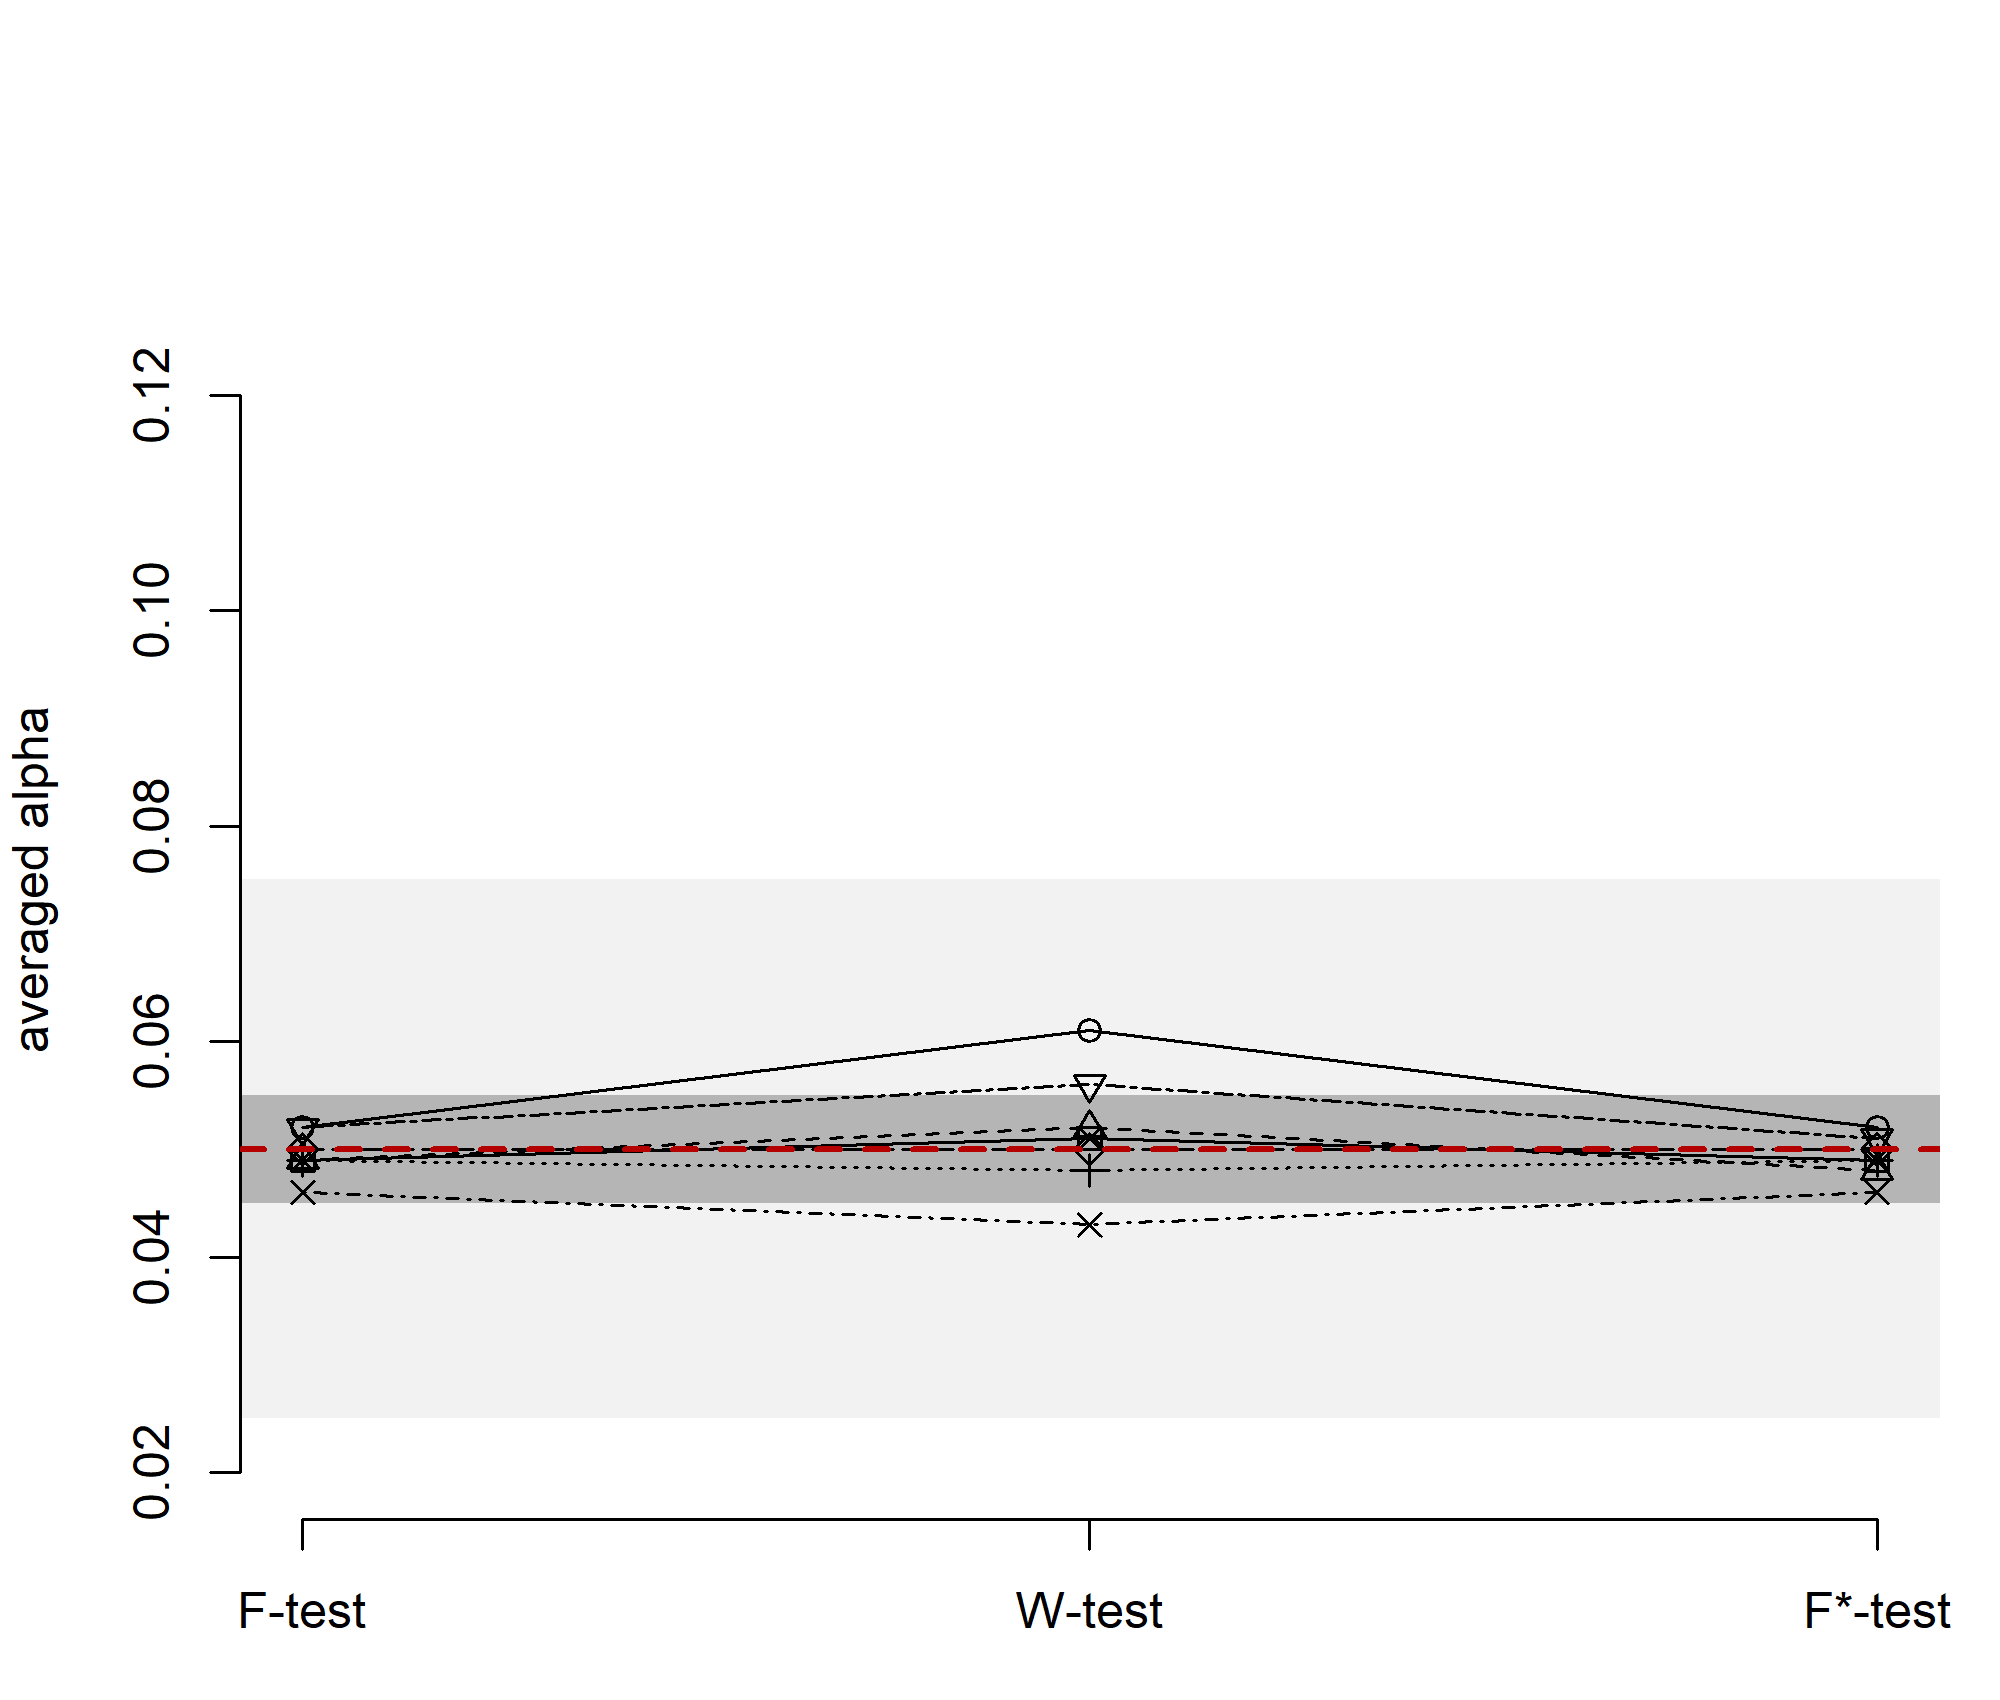
\includegraphics[width=400px]{Rmarkdown folder/Rmarkdown inputs/Fig1A} \caption{Type I error rate of the F-test, W-test and F*-test when there are equal SDs across groups and equal sample sizes (cell a in Table 1)}\label{fig:unnamed-chunk-2}
\end{figure}

\begin{figure}
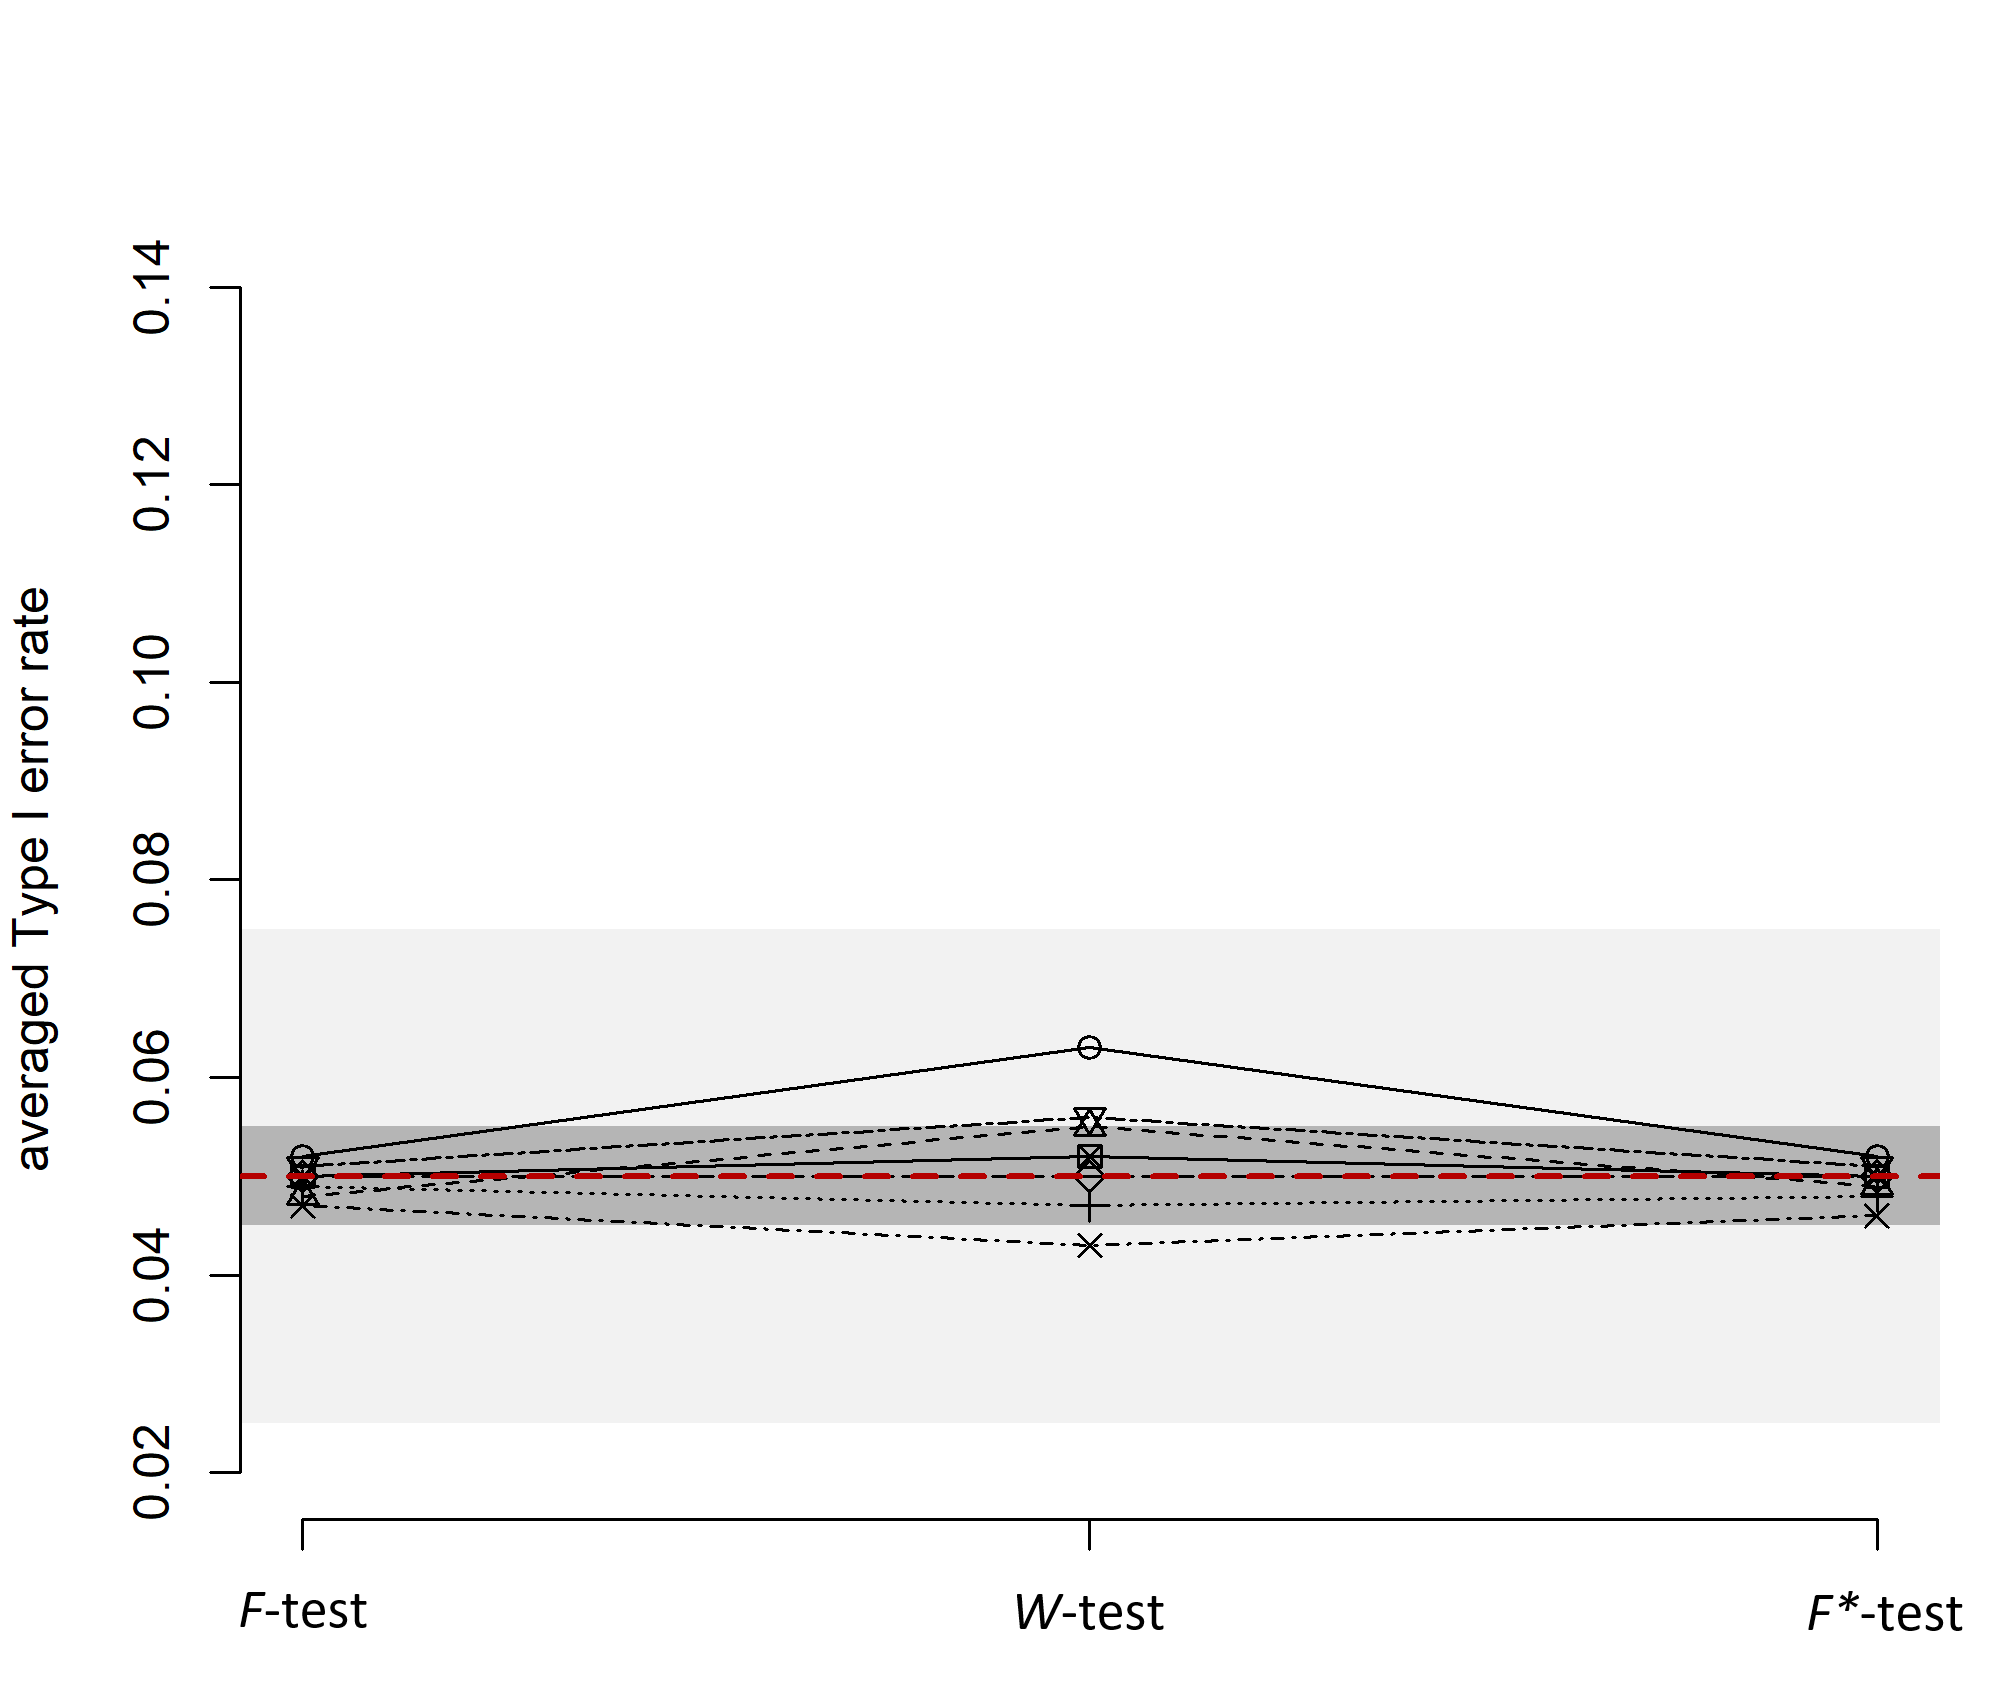
\includegraphics[width=400px]{Rmarkdown folder/Rmarkdown inputs/Fig1B} \caption{Type I error rate of the F-test, W-test and F*-test when there are equal SDs across groups and unequal sample sizes (cells b and c in Table 1)}\label{fig:unnamed-chunk-3}
\end{figure}

\begin{figure}
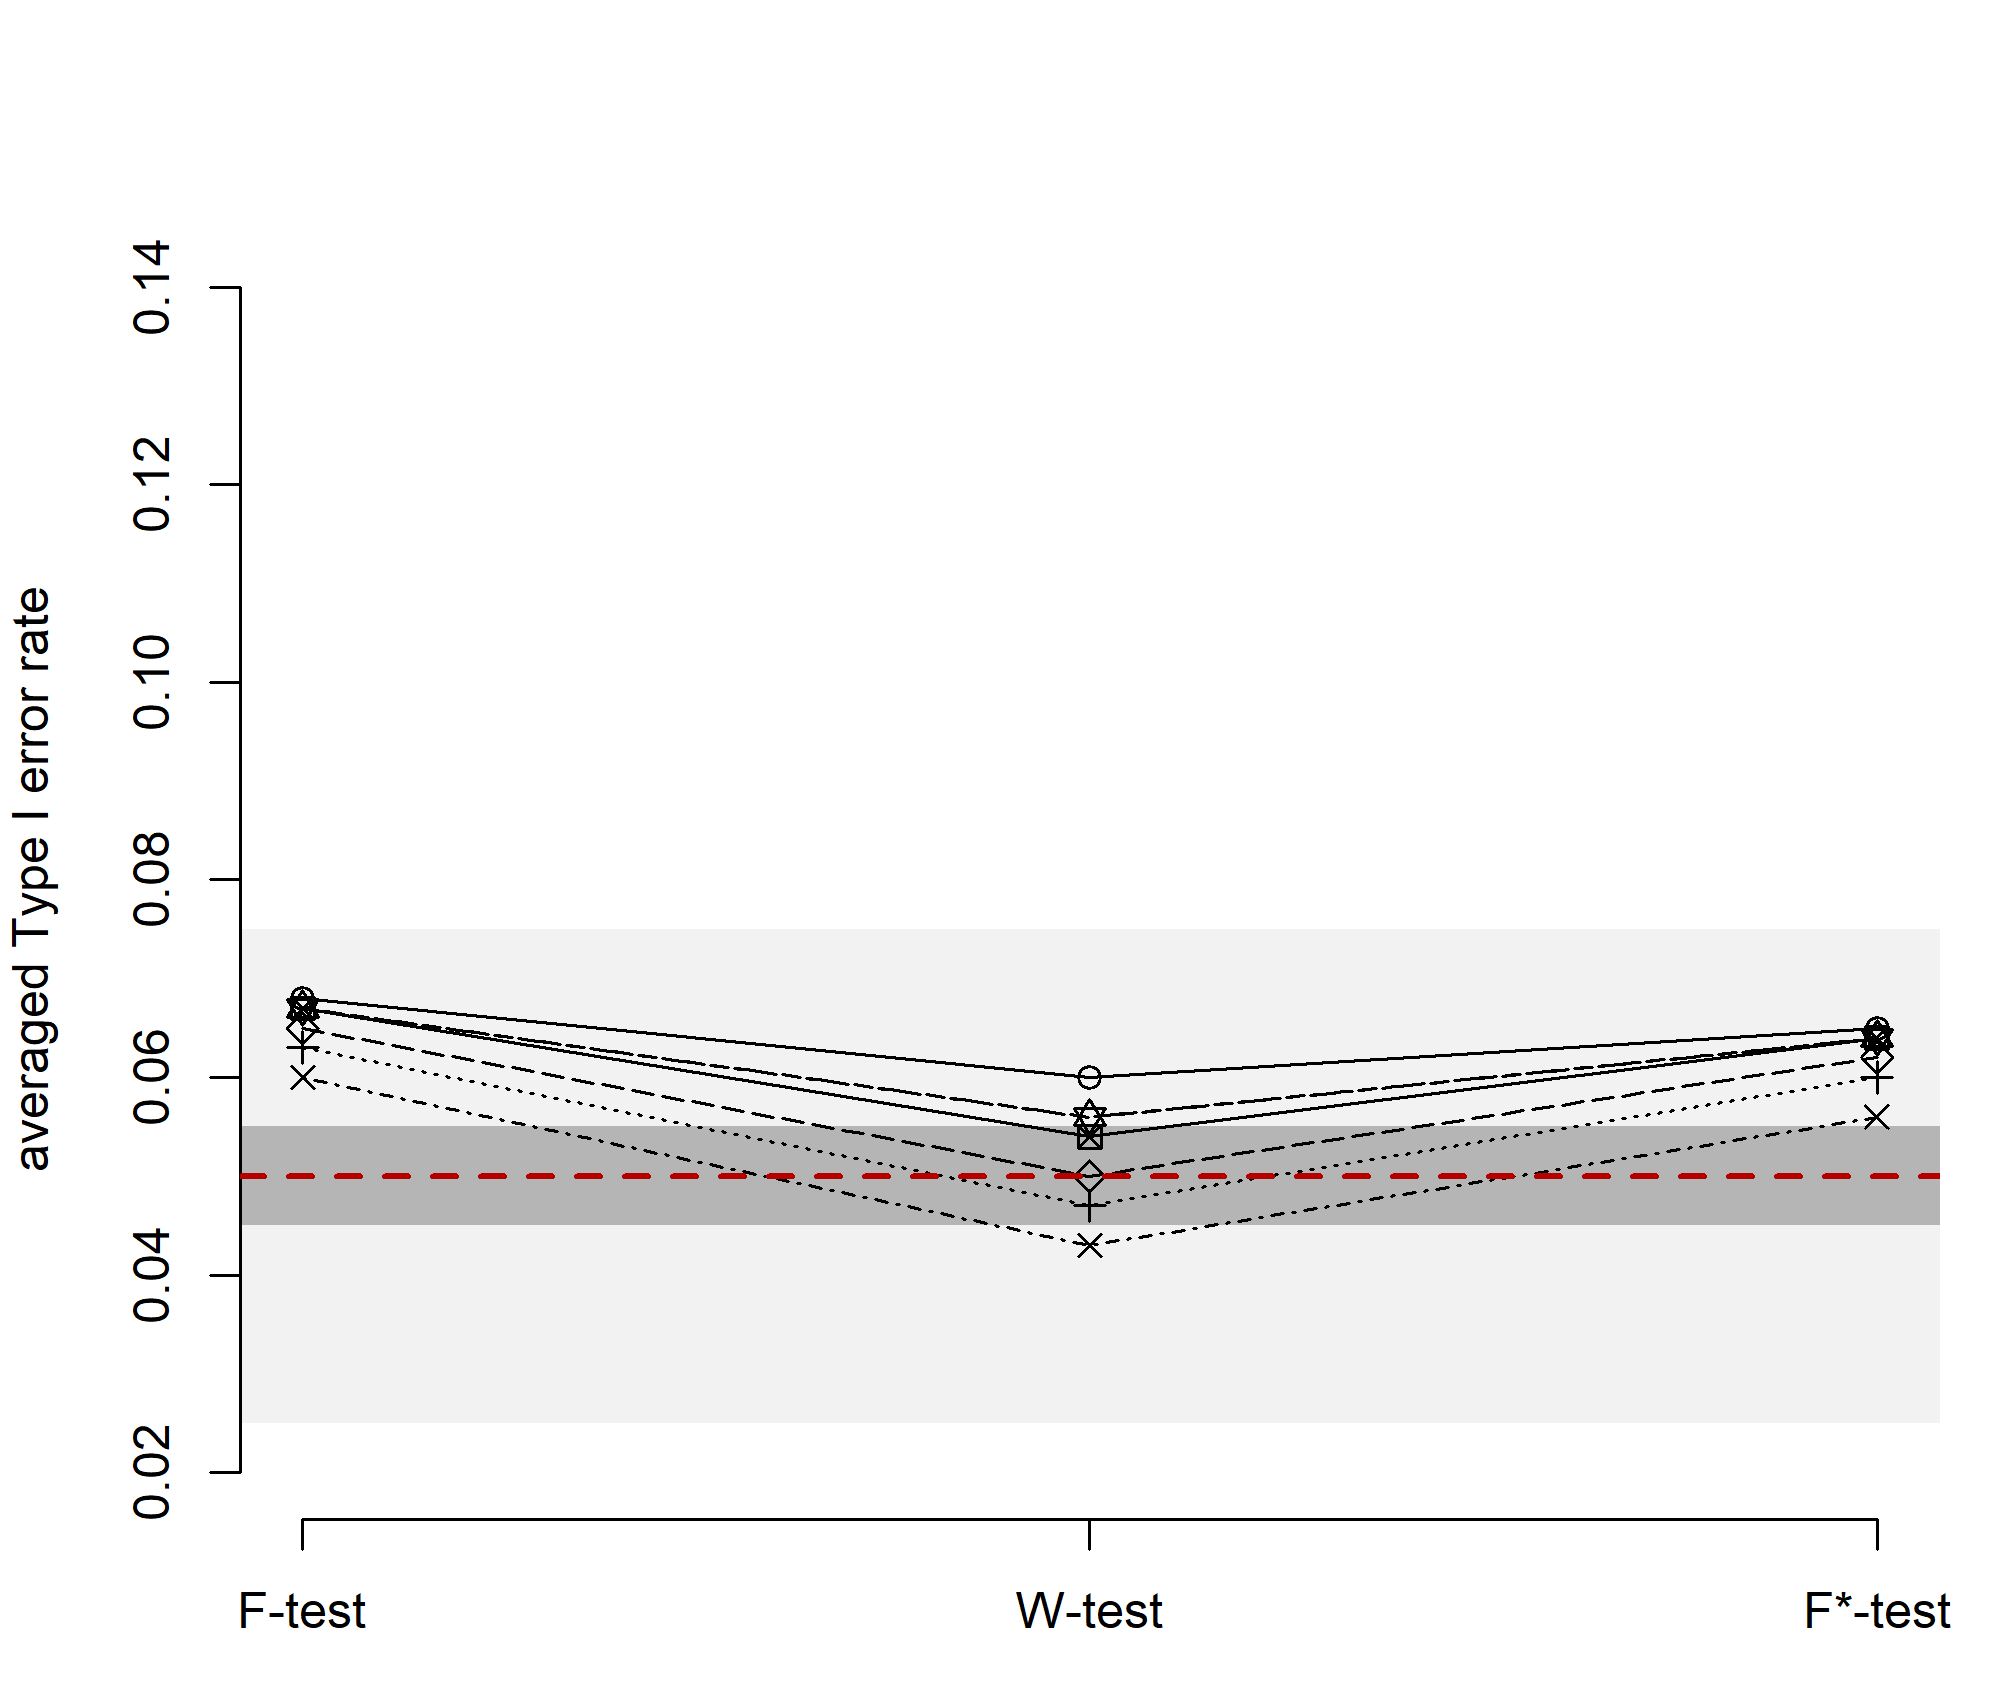
\includegraphics[width=400px]{Rmarkdown folder/Rmarkdown inputs/Fig1C} \caption{Type I error rate of the F-test, W-test and F*-test when there are unequal SDs across groups and equal sample sizes (cells d and g in Table 1)}\label{fig:unnamed-chunk-4}
\end{figure}

\begin{figure}
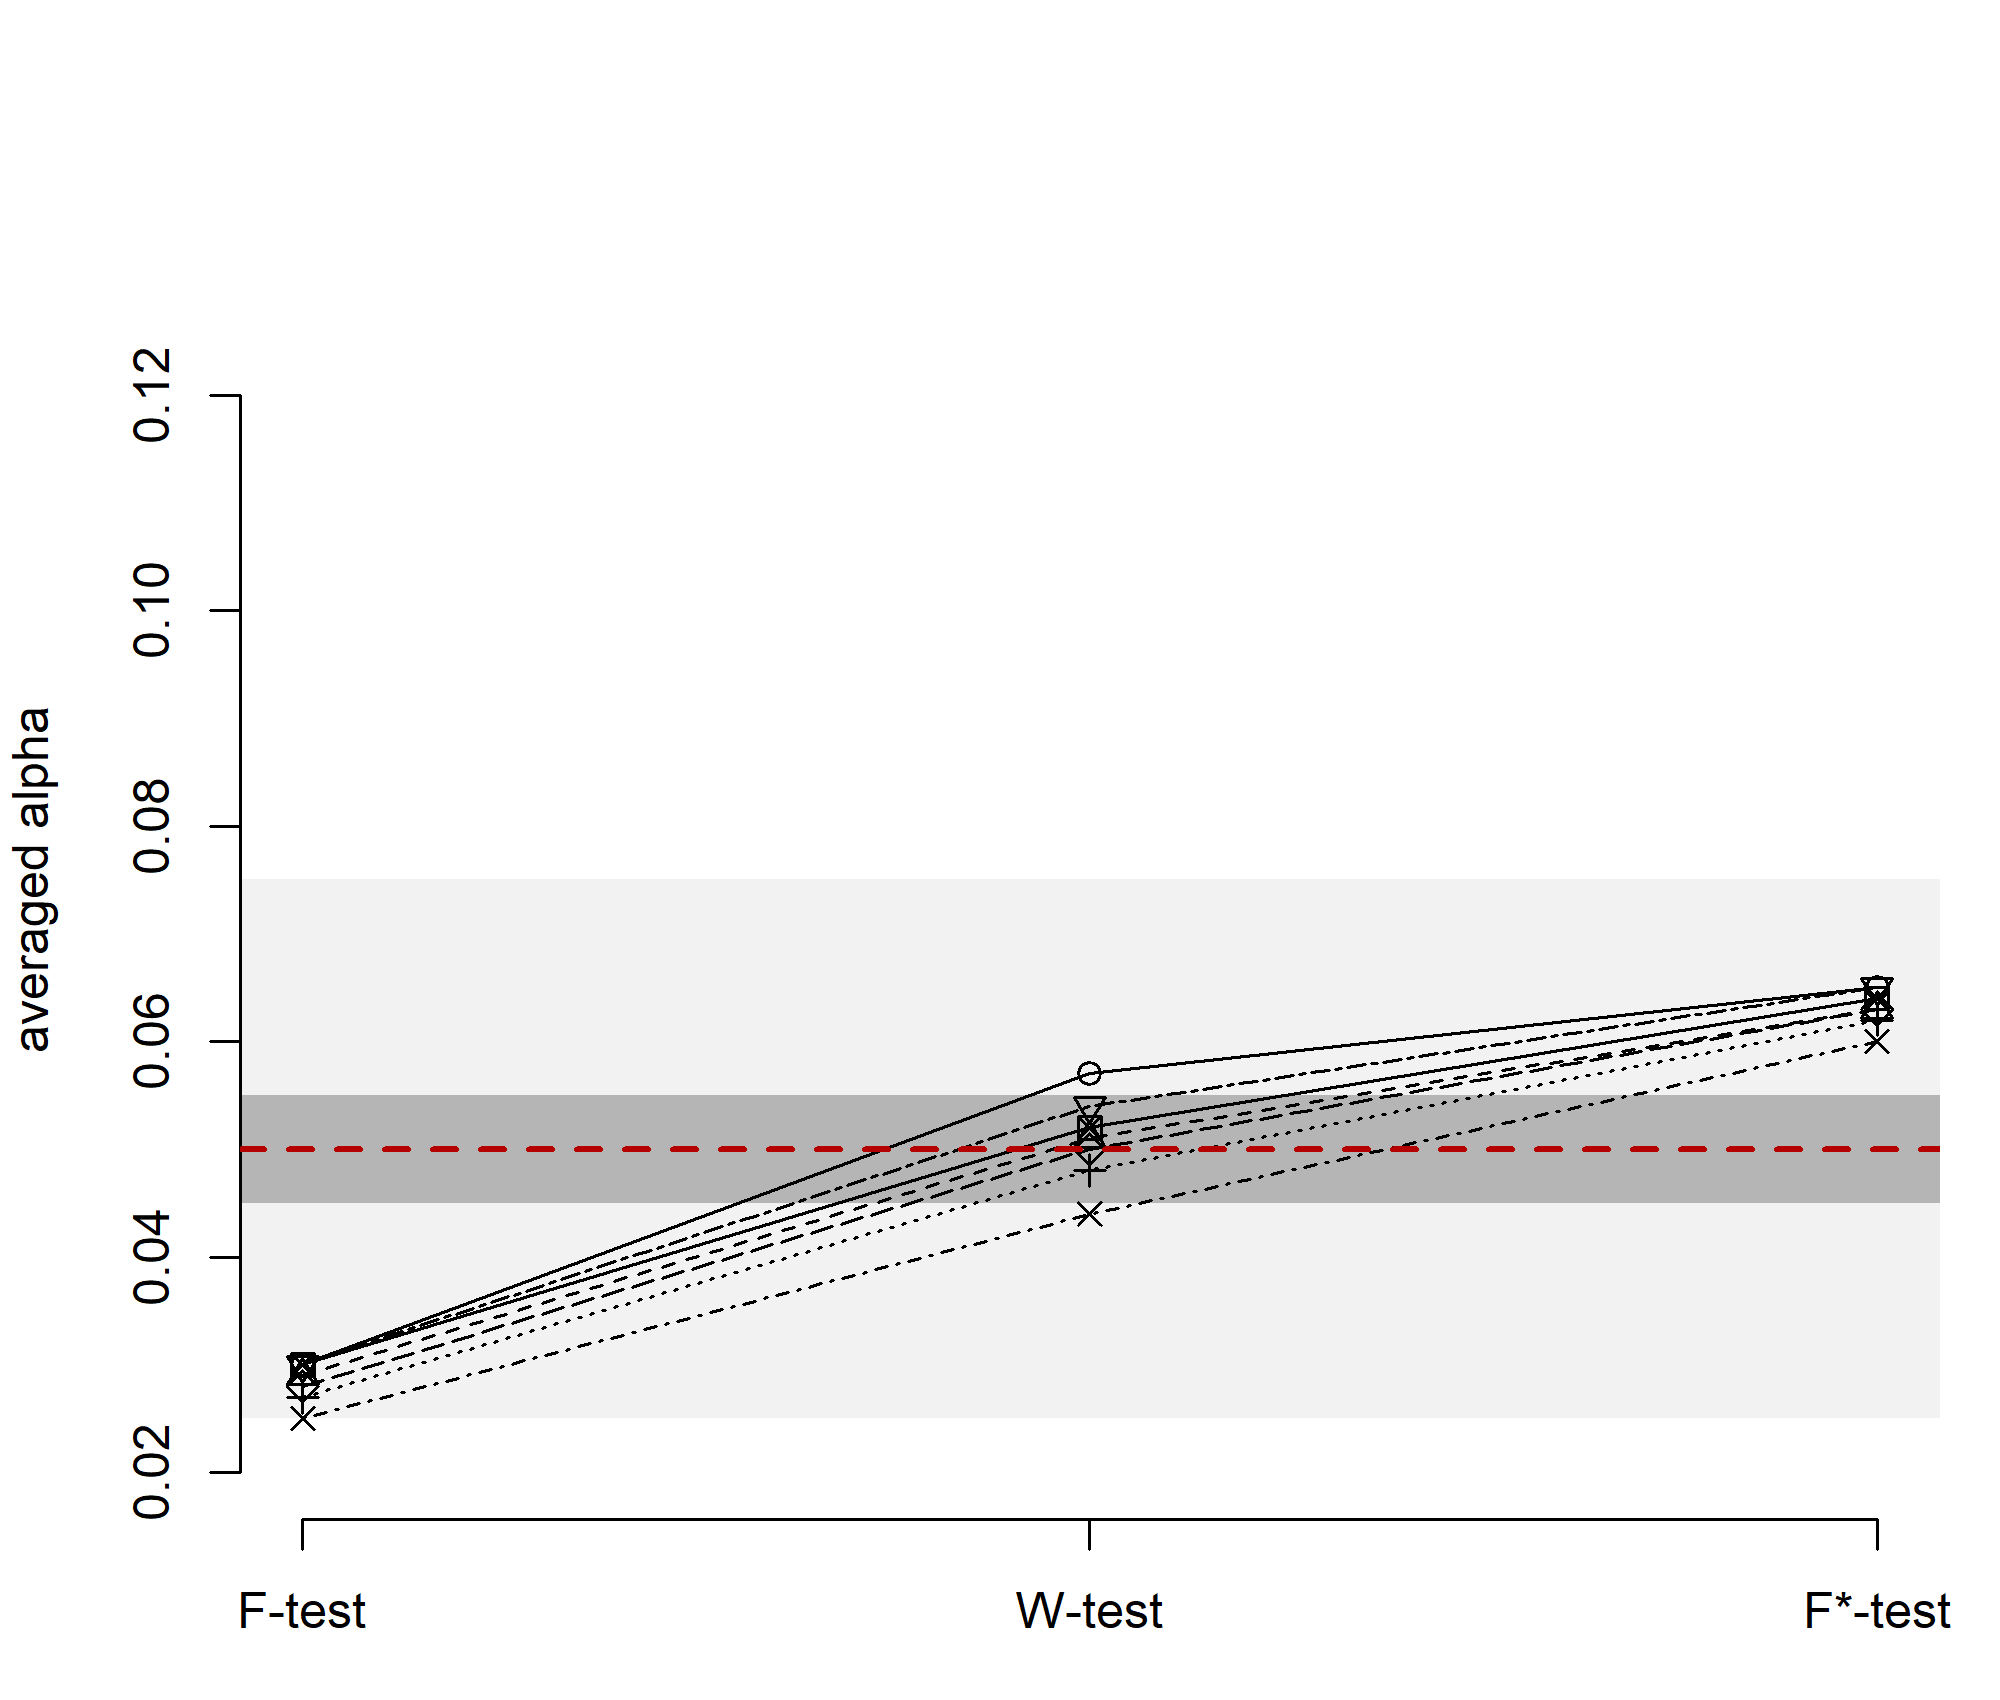
\includegraphics[width=400px]{Rmarkdown folder/Rmarkdown inputs/Fig1D} \caption{Type I error rate of the F-test, W-test and F*-test when there are unequal SDs across groups, and positive correlation between sample sizes and SDs (cells e and i in Table 1)}\label{fig:unnamed-chunk-5}
\end{figure}

\begin{figure}
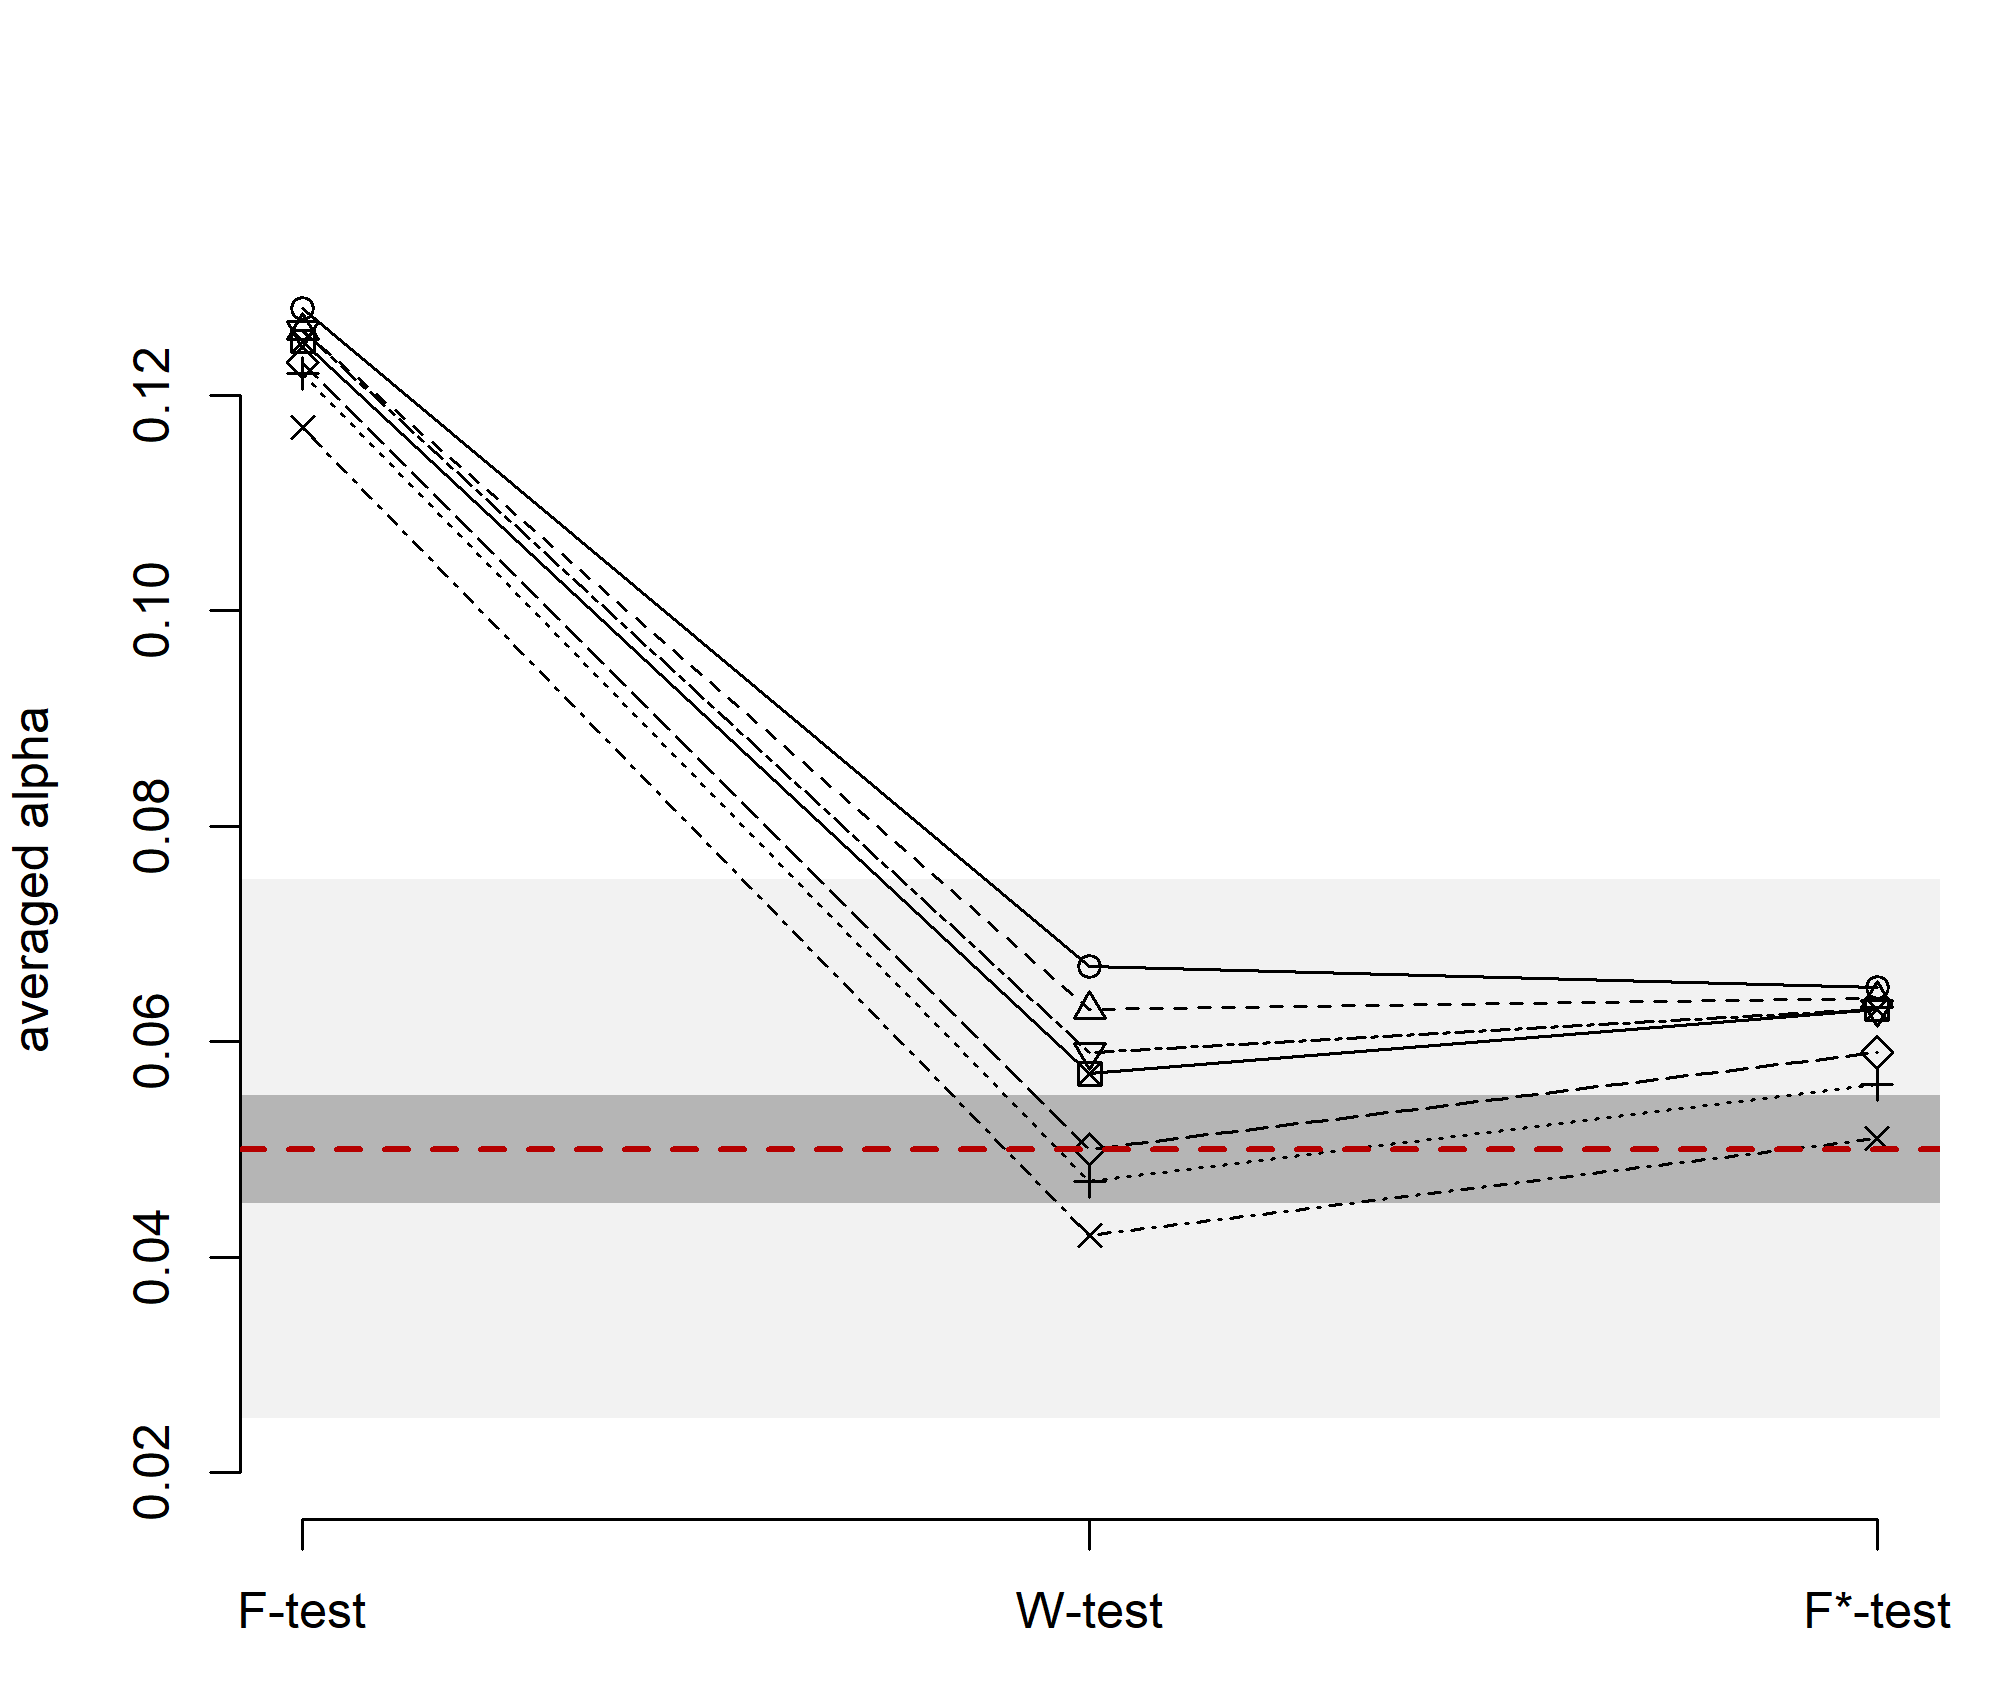
\includegraphics[width=400px]{Rmarkdown folder/Rmarkdown inputs/Fig1E} \caption{Type I error rate of the F-test, W-test and F*-test when there are unequal SDs across groups, and negative correlation between sample sizes and SDs (cells f and g in Table 1)}\label{fig:unnamed-chunk-6}
\end{figure}

In Figures 2 and 3 (cells a, b, and c in Table 1), the population variance is equal between all groups, so the homoscedasticity assumption is met. The \emph{F}-test and \emph{F*}-test only marginally deviate from the nominal 5\%, regardless of the underlying distribution and the \emph{SD}-ratio. The \emph{W}-test also only marginally deviates from the nominal 5\%, except under asymmetry (the tests becomes a little more liberal) or extremely heavy tails (the test becomes a bit more conservative), consistently with observations in Harwell et al. (1992). However, deviations don't exceed the liberal criterion of Bradley (1978).

In Figures 4, 5, and 6 (cells d to i, Table 1) the population variance is unequal between groups, so that the homoscedasticity assumption is not met. When sample sizes are equal across groups (Figure 4) and when there is a positive correlation between sample sizes and \emph{SDs} (Figure 5), the Type I error rate of the \emph{W}-test is closer to the nominal 5\% than the Type I error rate of the \emph{F*}-test and the \emph{F}-test, the latter which is consistently at the lower limit of the liberal interval suggested by Bradley, in line with Harwell et al. (1992), Glass et al. (1972), Nimon (2012) and Overall et al. (1995). Heteroscedasticity does not impact the Type I error rate of the \emph{W}-test, regardless of the distribution (the order of the distribution shape remains the same in all conditions).

When there is a negative correlation between sample sizes and \emph{SDs} (Figure 6), the Type I error rate of the \emph{F*}-test is slightly closer of the nominal 5\% than the Type I error rate of the \emph{W}-test, for which the distributions (more specifically, the skewness) has a larger impact on the Type I error rate than when there is homoscedasticity. This is consistent with conclusions by Lix et al. (1996) about the Alexander-Govern and the James' second order tests (which return very similar results as the \emph{W}-test, as we already mentioned). However, both tests still perform relatively well, contrary to the \emph{F}-test that is much too liberal, in line with observations by Harwell et al. (1992), Glass et al. (1972), Nimon (2012) and Overall et al. (1995).

\hypertarget{conclusions}{%
\subsubsection{Conclusions}\label{conclusions}}

We can draw the following conclusions for the Type I error rate:

\begin{enumerate}
\def\labelenumi{\arabic{enumi})}
\tightlist
\item
  When all assumptions are met, all tests perform adequately.\\
\item
  When variances are equal between groups and distributions are not normal, the \emph{W}-test is a little less efficient than both the \emph{F}-test and the \emph{F*}-test, but departures from the nominal 5\% Type I error rate never exceed the liberal criterion of Bradley (1978).\\
\item
  When the assumption of equal variances is violated, the \emph{W}-test clearly outperforms both the \emph{F*}-test (which is more liberal) and the \emph{F}-test (which is either more liberal or more conservative, depending on the \emph{SDs} and \emph{SD} pairing).\\
\item
  The last conclusion generally remains true when both the assumptions of equal variances and normality are not met.
\end{enumerate}

\hypertarget{statistical-power-for-the-f-test-w-test-and-f-test}{%
\subsection{\texorpdfstring{Statistical power for the \emph{F}-test, \emph{W}-test, and \emph{F}*-test}{Statistical power for the F-test, W-test, and F*-test}}\label{statistical-power-for-the-f-test-w-test-and-f-test}}

As previously mentioned, the statistical power (1-\(\beta\)) of a test is the long-run probability of observing a statistically significant result when there is a true effect in the population. We assessed the power of the \emph{F}-test, \emph{W}-test and \emph{F*}-test under 1280 scenarios, while using the nominal alpha level of 5\%. In all scenarios, the last group was extracted from a population that has a higher mean than the population from where were extracted all other groups (\(\mu_k = \mu_j+1\)). Because of this, in some scenarios there is a positive correlation between the \emph{SD} and the mean (i.e.~the last group has the largest \emph{SD} and the largest mean) and in other scenarios, there is a negative correlation between \emph{SD} and the mean (i.e.~the last group has the smallest \emph{SD} and the largest mean). As we know that the correlation between the \emph{SD} and the mean matters for the \emph{W}-test (see Liu, 2015), the 9 subconditions in Table 1 were analyzed separately.

We computed two main outcomes: the consistency and the power. The consistency refers to the relative difference between the observed power and the nominal power, divided by the expected power:
\begin{equation} 
Consistency=\frac{0-E}{E}
\label{eq:RDPWtest}
\end{equation}

When consistency equals zero, the observed power is consistent with the nominal power (under the parametric assumptions of normality and homoscedasticity); a negative consistency shows that the observed power is lower than the expected power; and a positive consistency shows that the observed power is higher than the expected power.

\begin{figure}
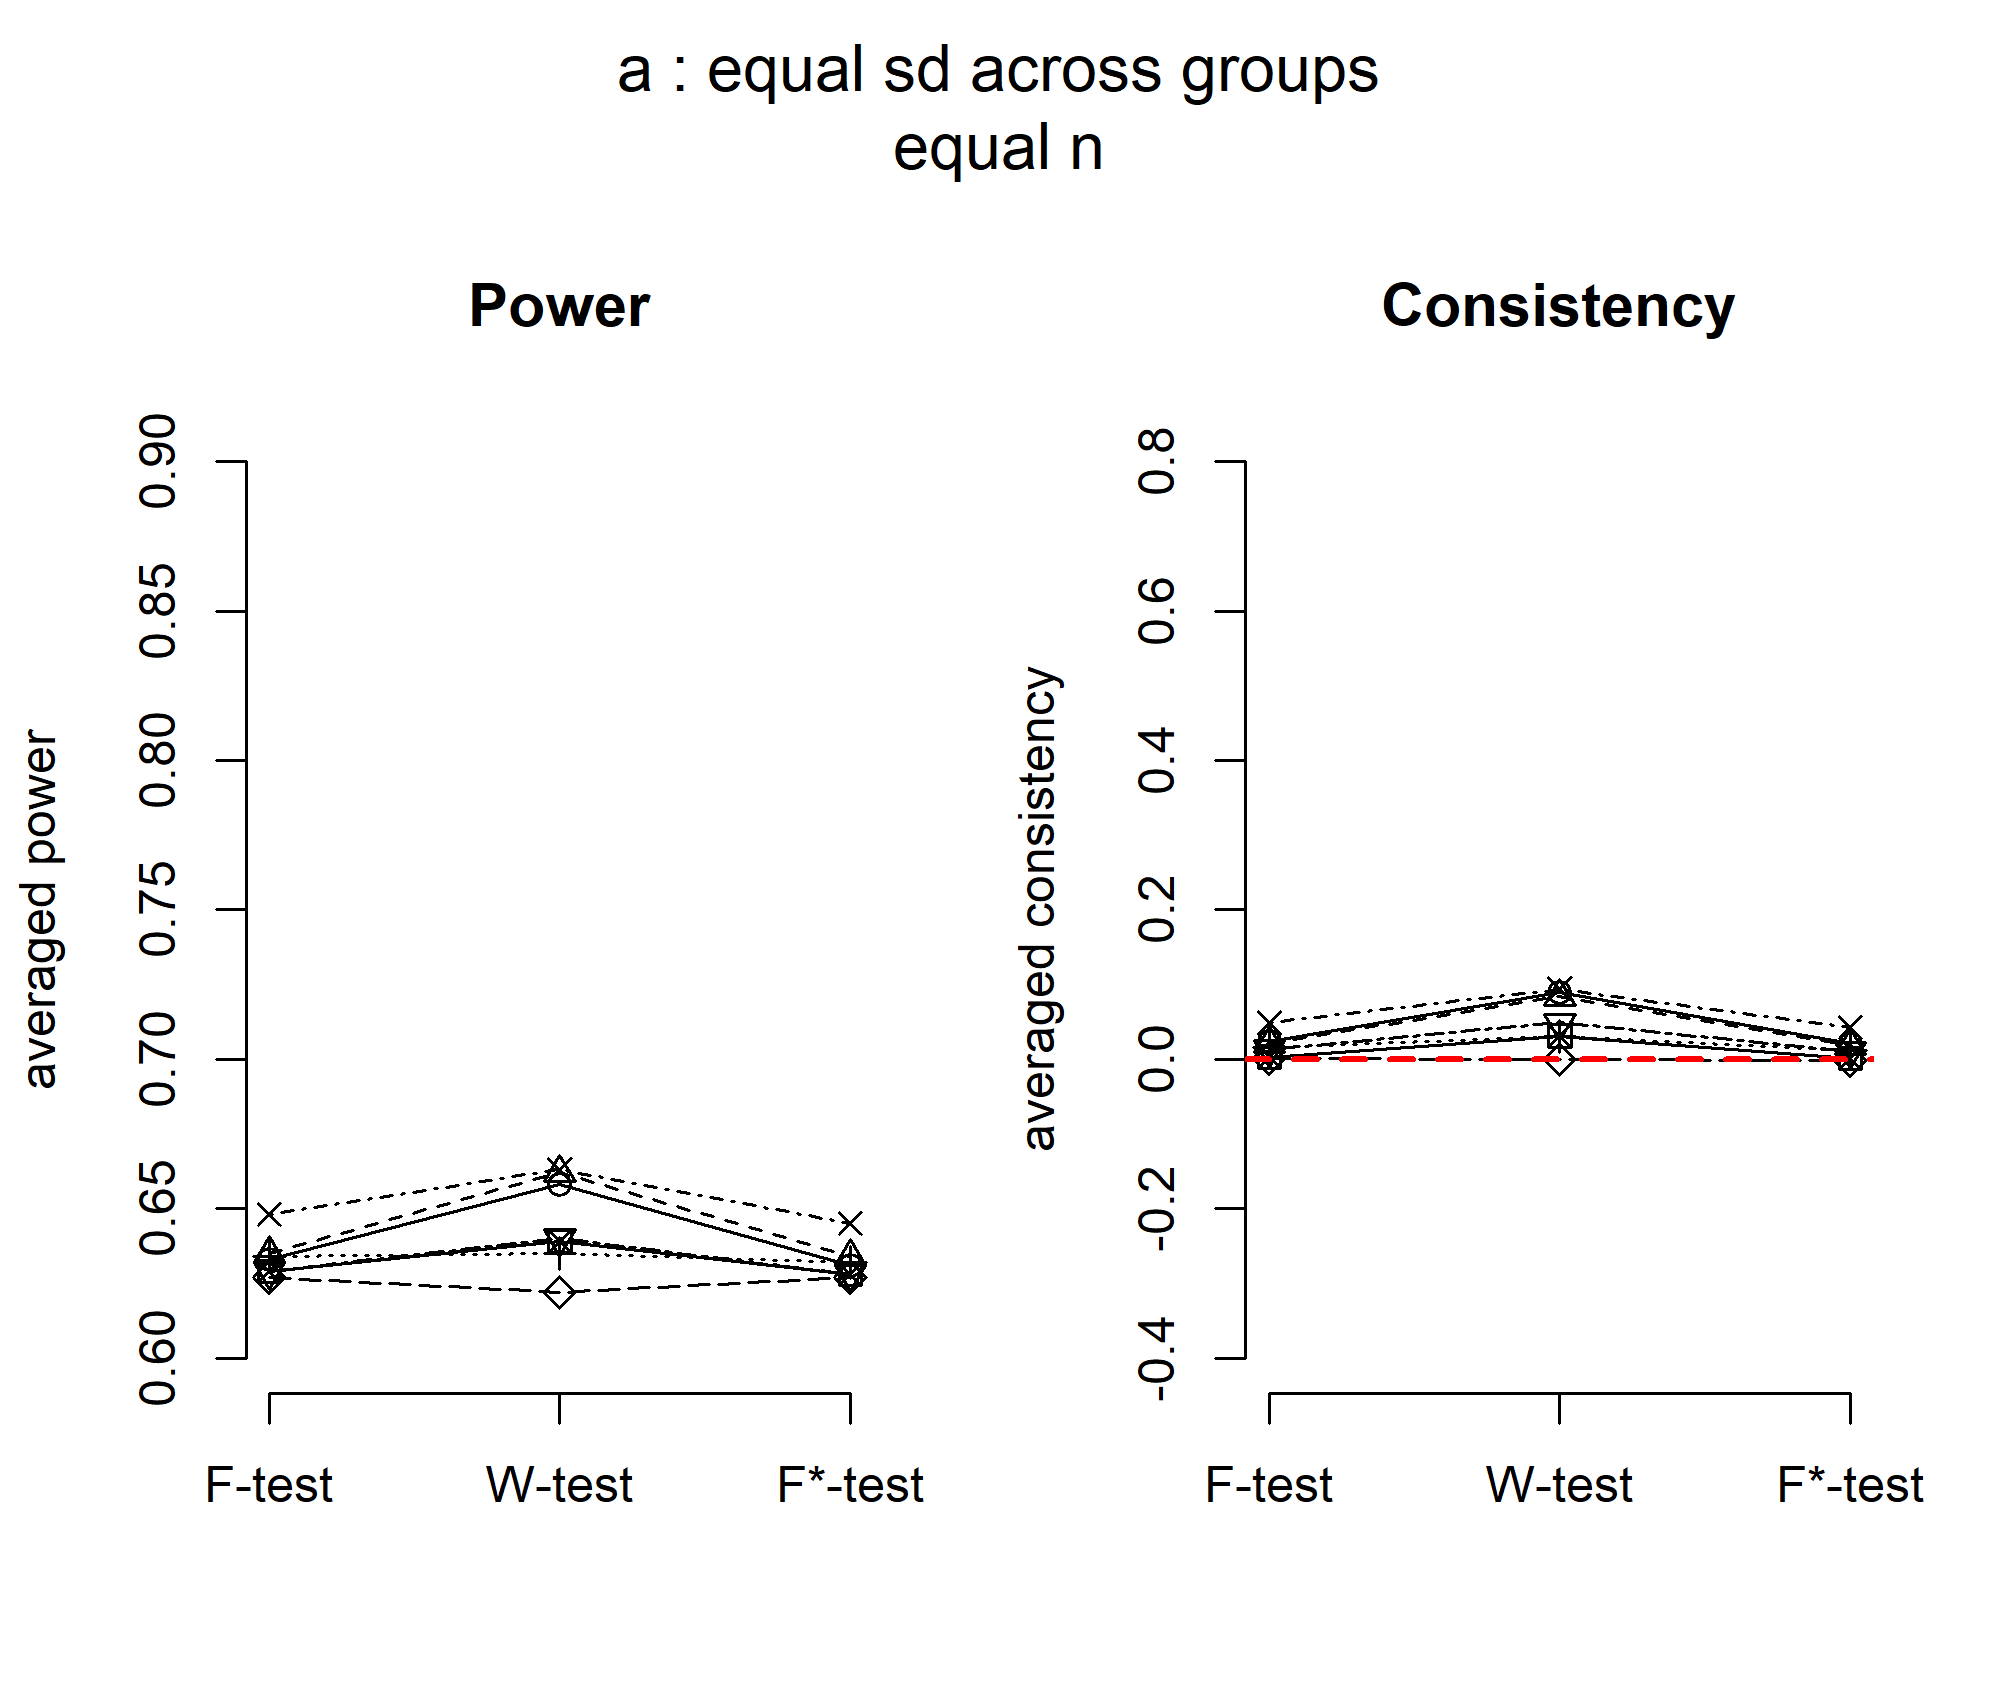
\includegraphics[width=400px]{Rmarkdown folder/Rmarkdown inputs/Fig2a} \caption{Power and consistency of the F-test, W-test and F*-test when there are equal SDs across groups and equal sample sizes (cell a in Table 1)}\label{fig:unnamed-chunk-7}
\end{figure}

\begin{figure}
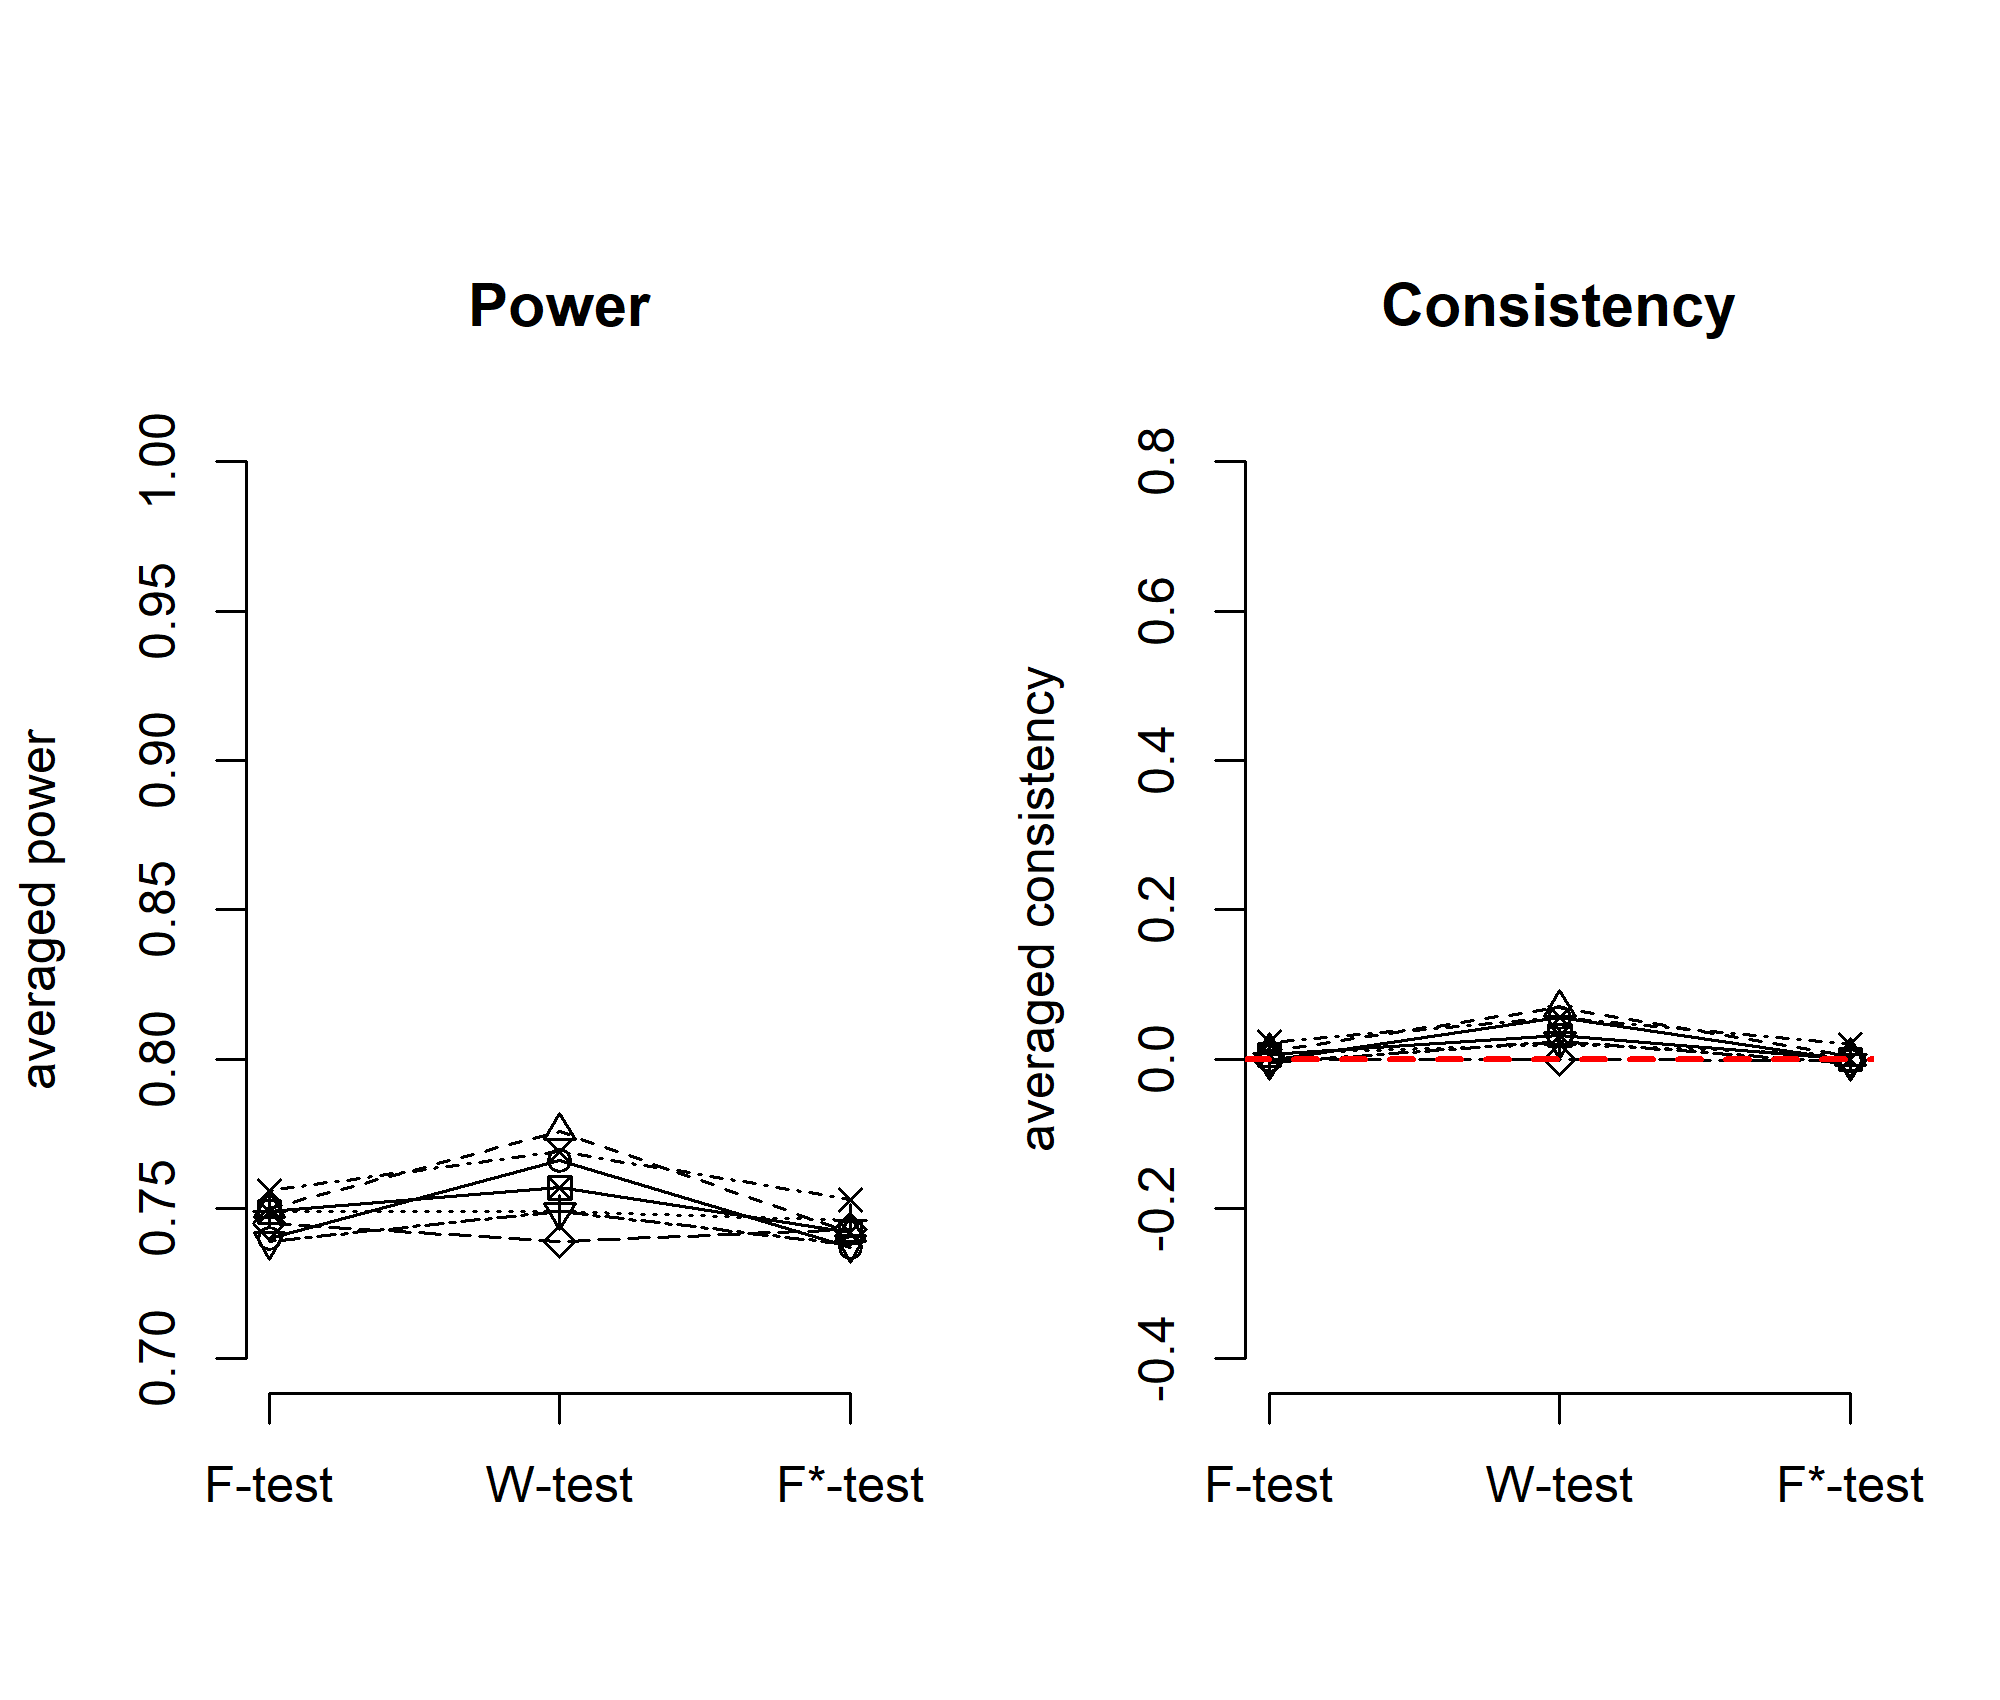
\includegraphics[width=400px]{Rmarkdown folder/Rmarkdown inputs/Fig2b} \caption{Power and consistency of the F-test, W-test and F*-test when there are equal SDs across groups, and positive correlation between sample sizes and means (cell b in Table 1)}\label{fig:unnamed-chunk-8}
\end{figure}

\begin{figure}
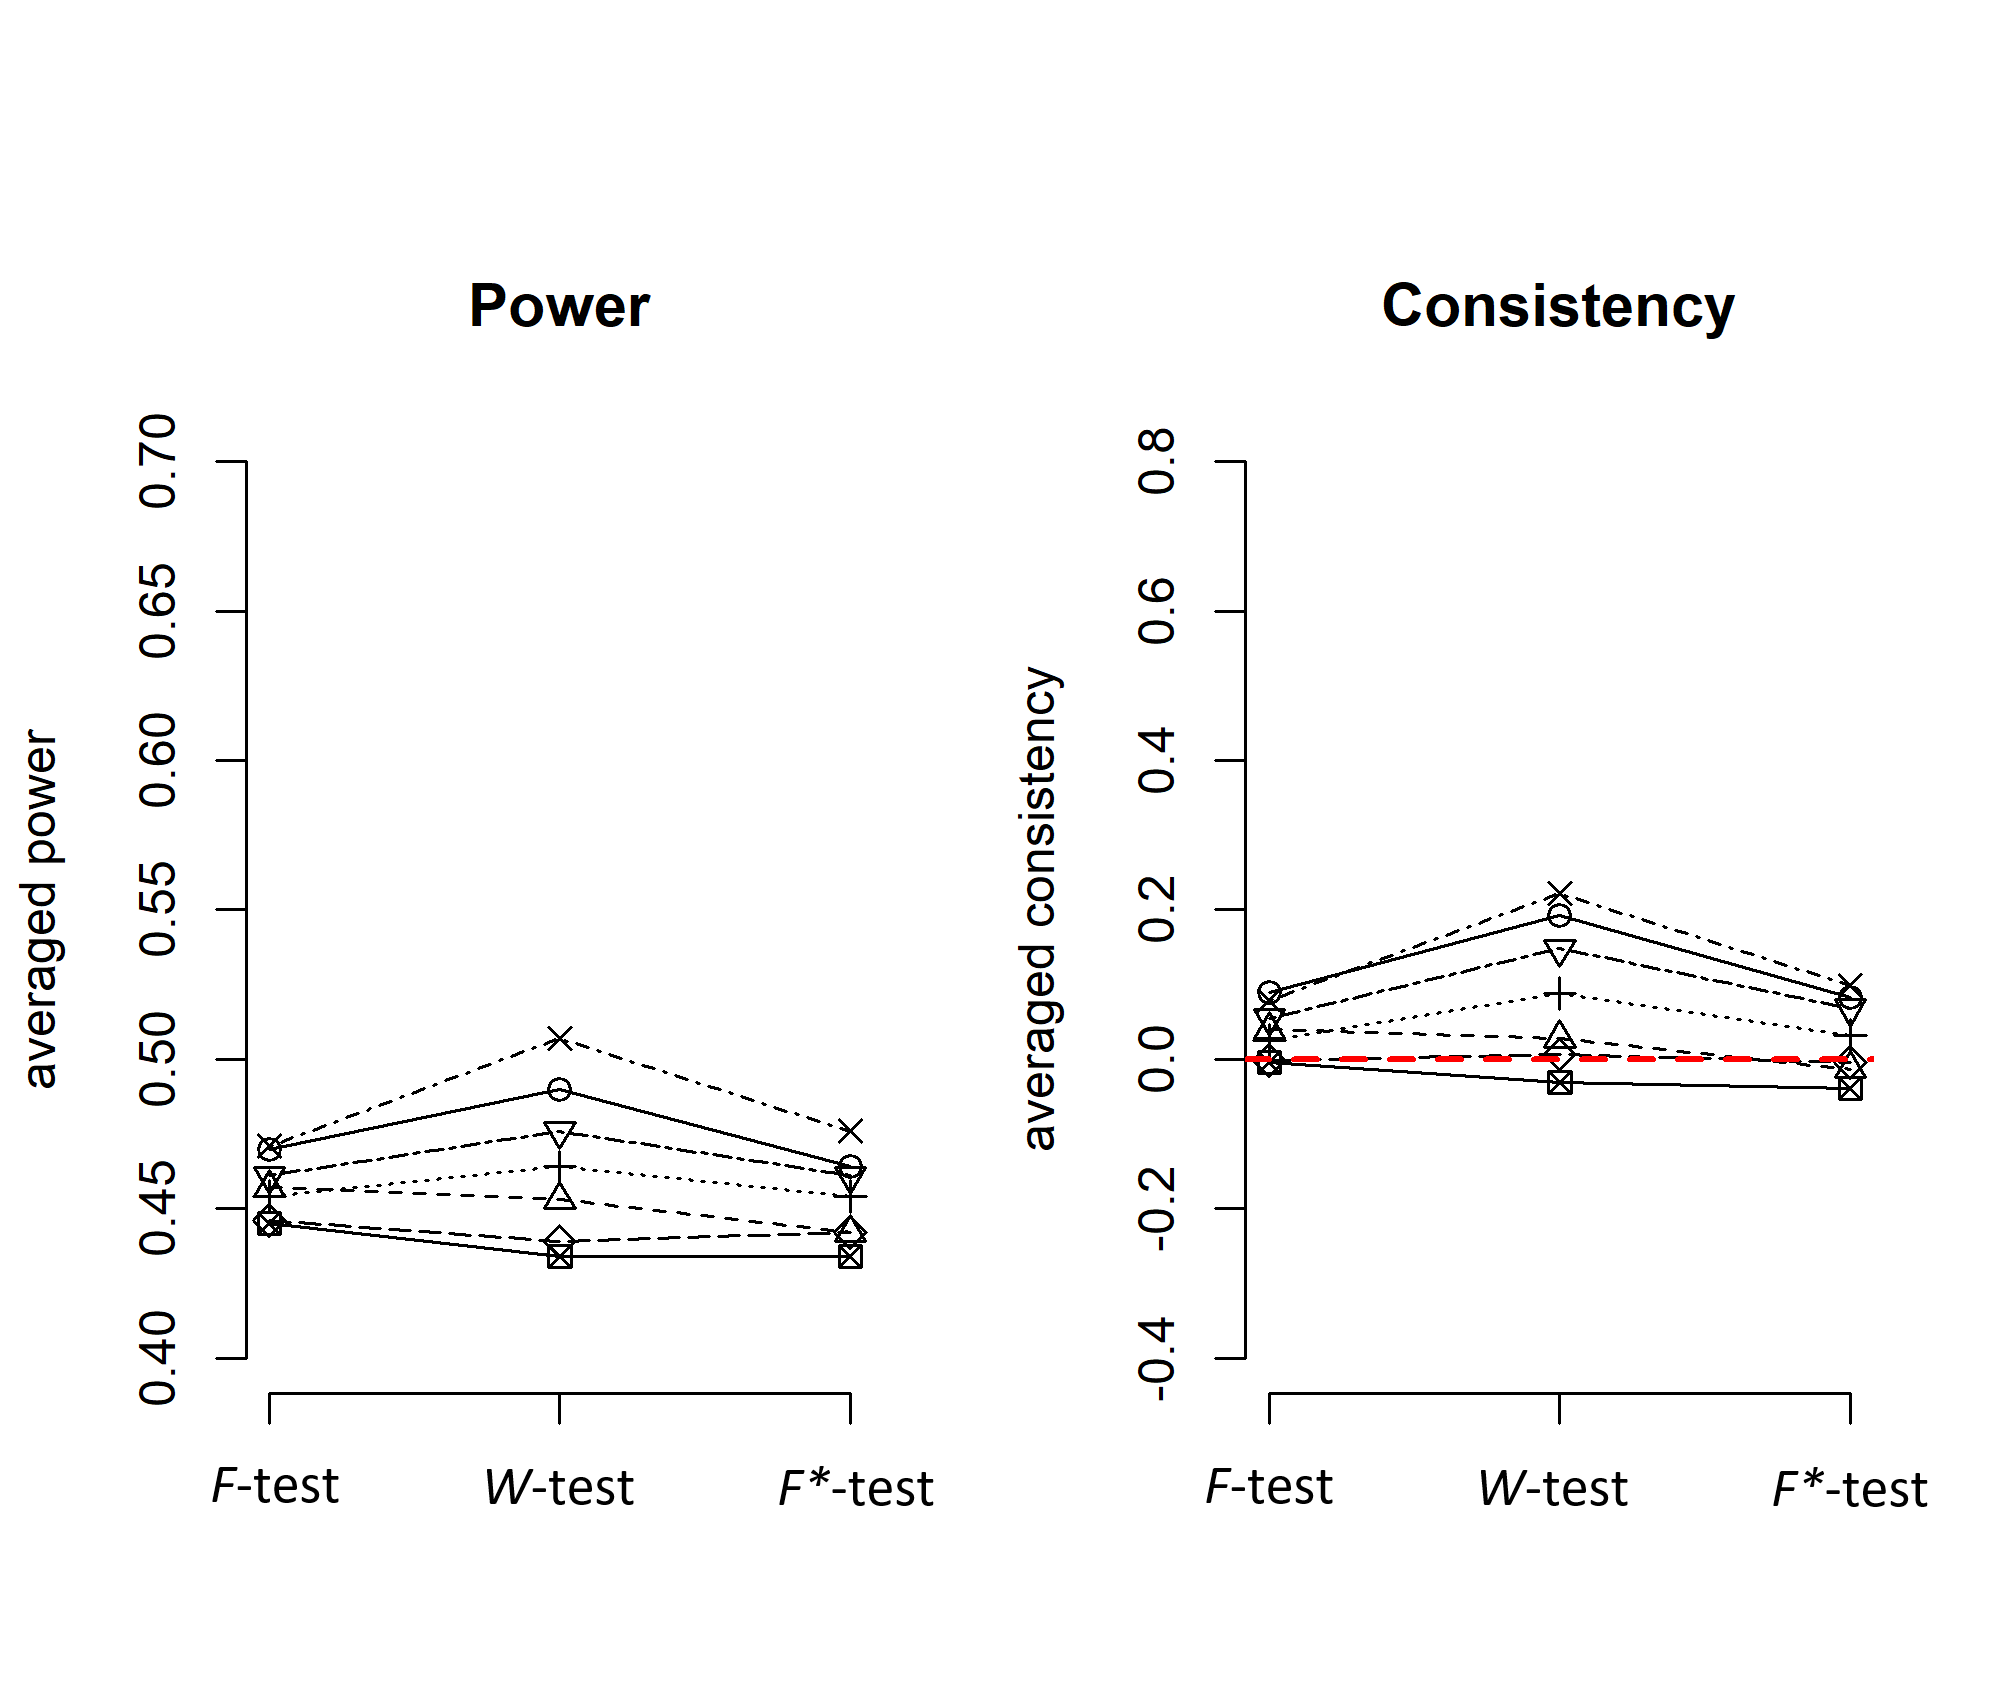
\includegraphics[width=400px]{Rmarkdown folder/Rmarkdown inputs/Fig2c} \caption{Power and consistency of the F-test, W-test and F*-test when there are equal SDs across groups, and negative correlation between sample sizes and means (cell c in Table 1)}\label{fig:unnamed-chunk-9}
\end{figure}

\begin{figure}
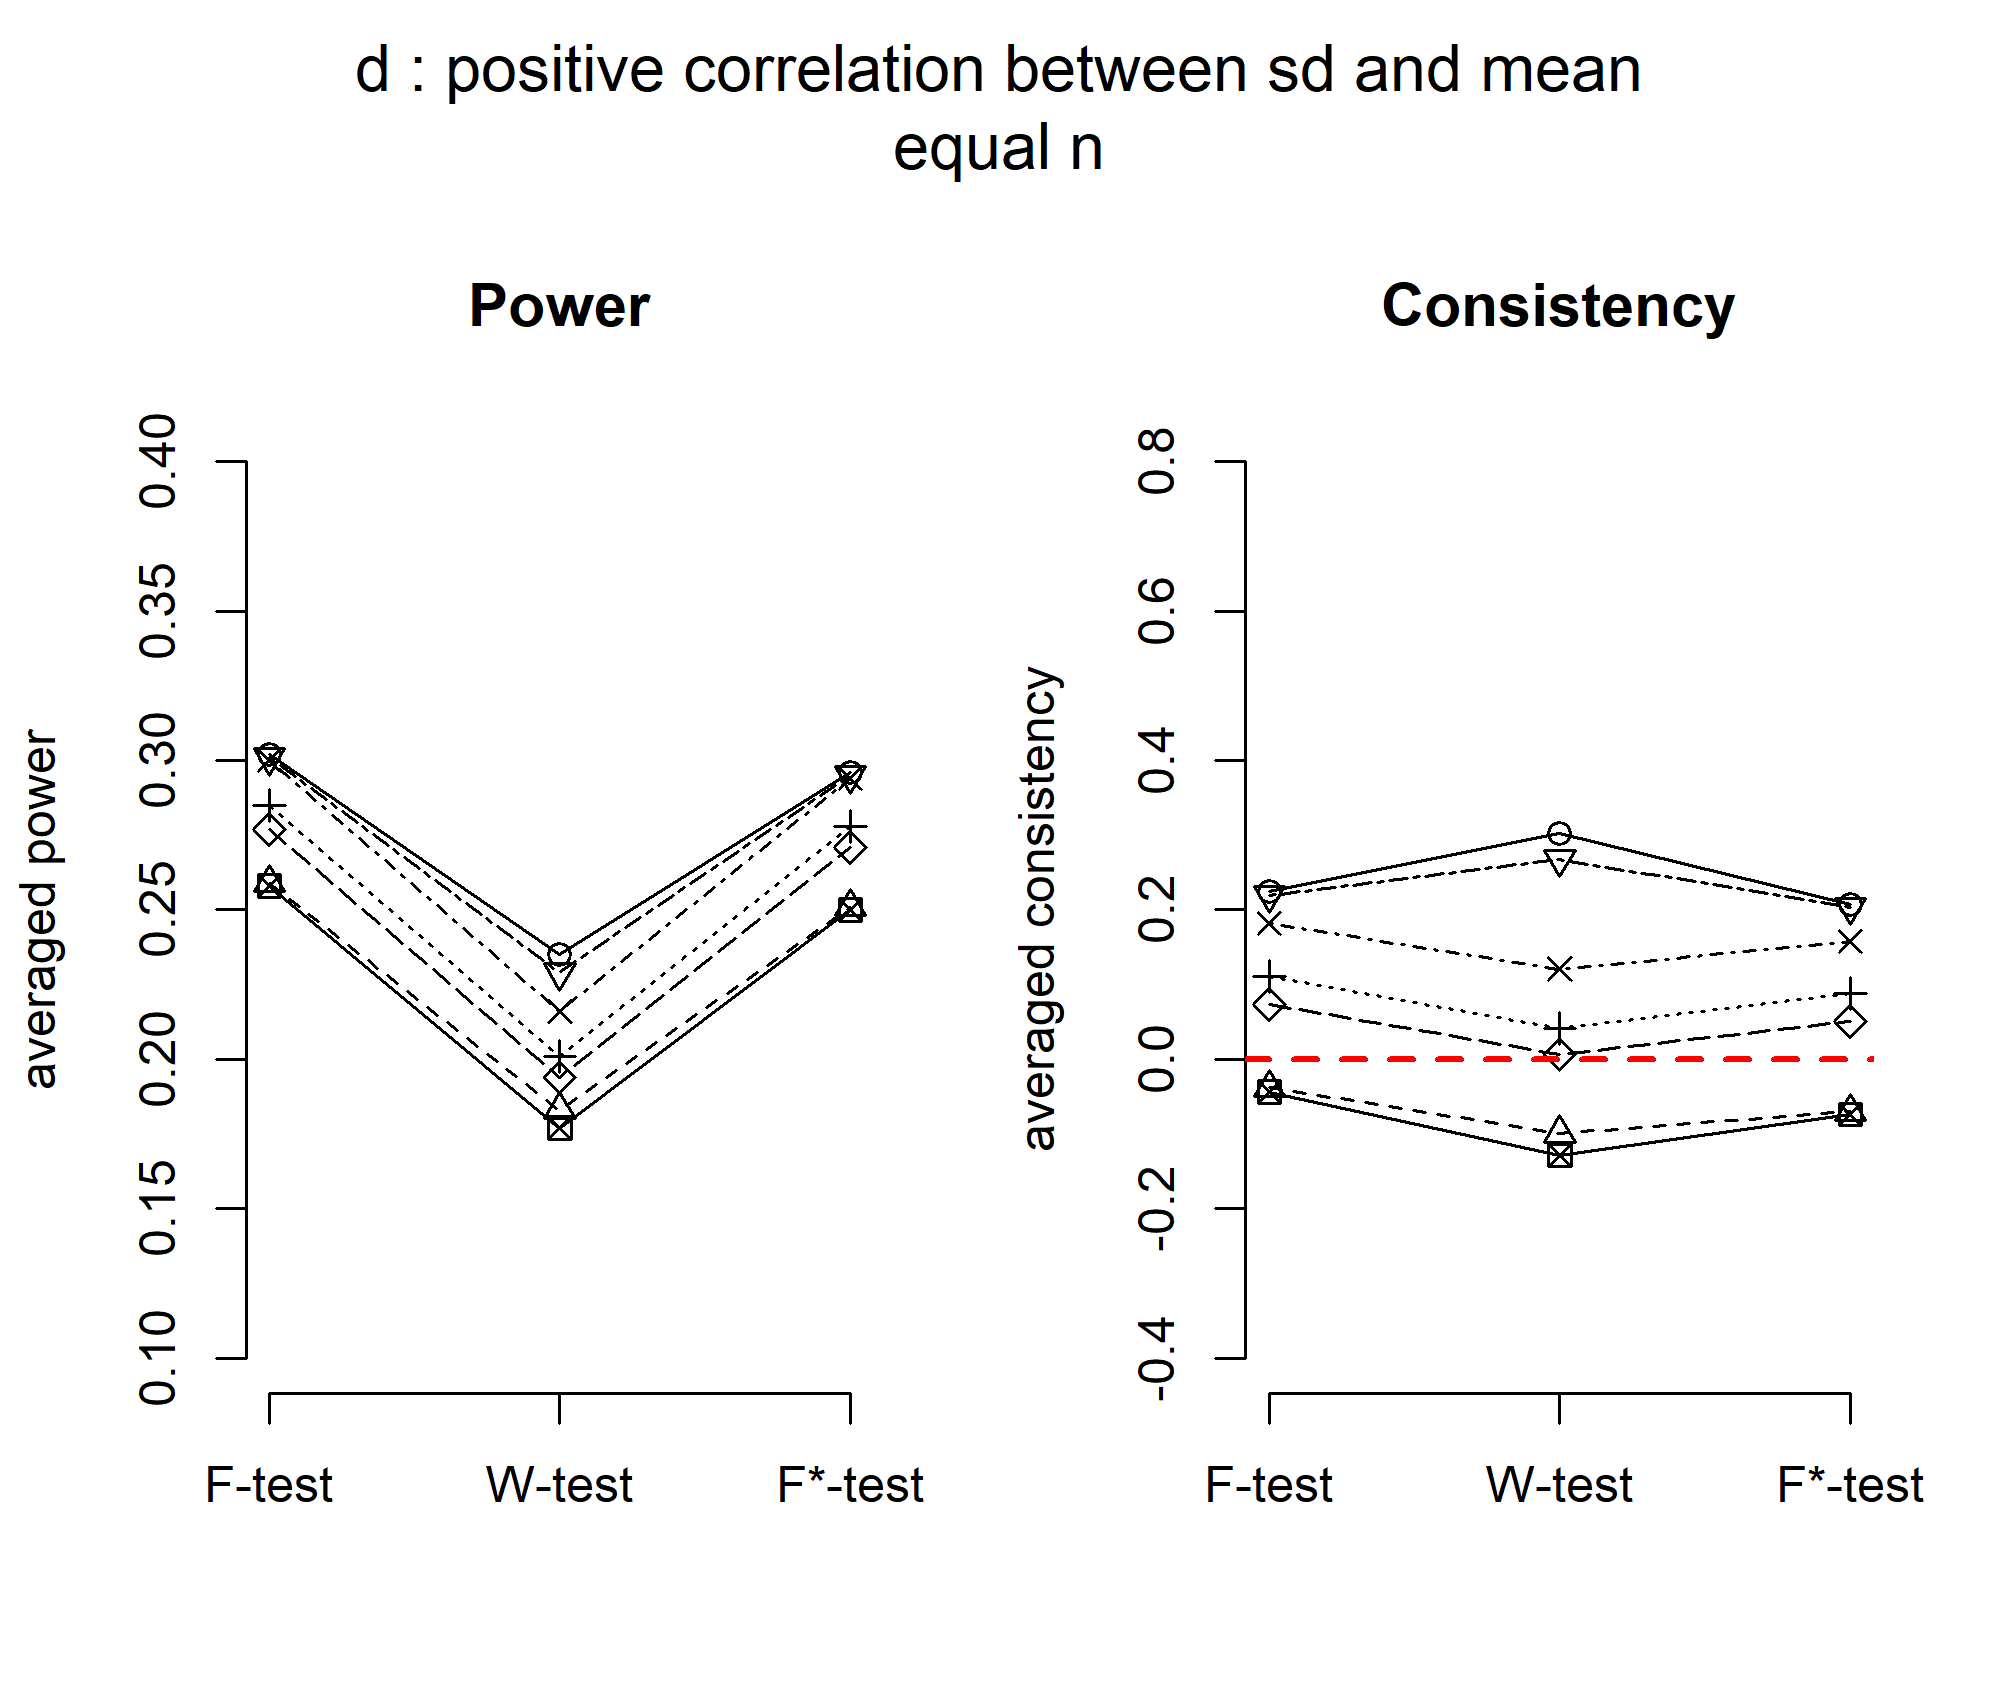
\includegraphics[width=400px]{Rmarkdown folder/Rmarkdown inputs/Fig2d} \caption{Power and consistency of the F-test, W-test and F*-test when there are unequal SDs across groups, positive correlation between SDs and means, and equal sample sizes across groups (cell d in Table 1)}\label{fig:unnamed-chunk-10}
\end{figure}

\begin{figure}
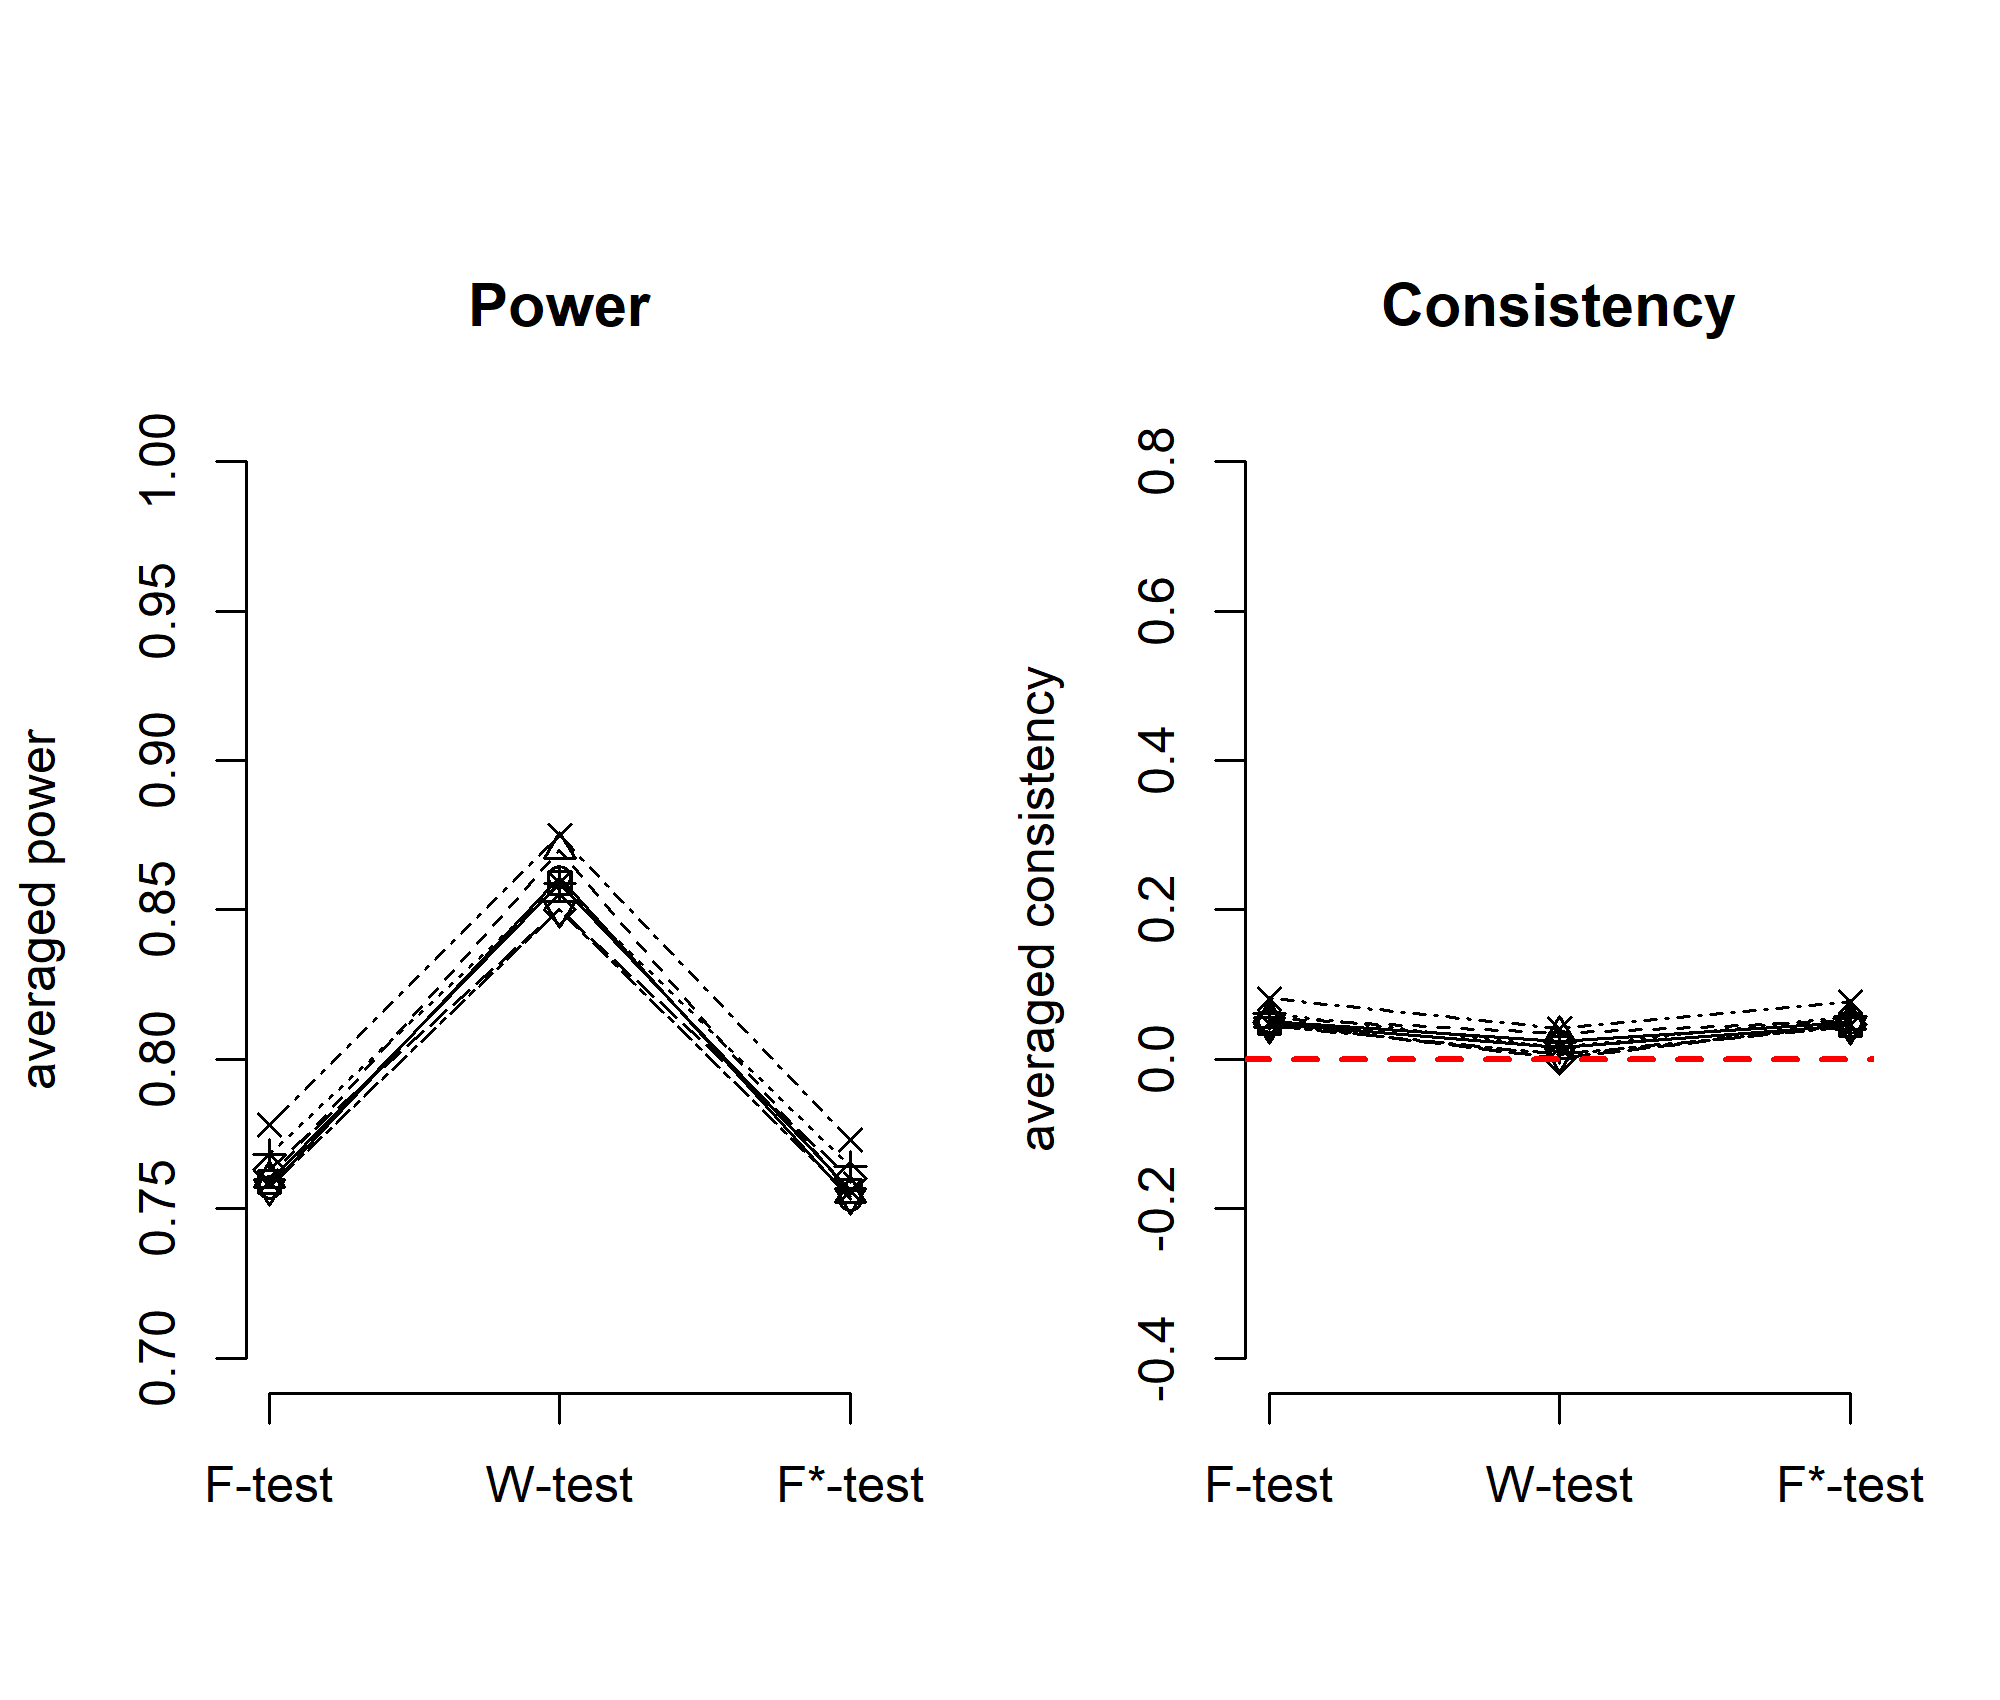
\includegraphics[width=400px]{Rmarkdown folder/Rmarkdown inputs/Fig2e} \caption{Power and consistency of the F-test, W-test and F*-test when there are unequal SDs across groups, negative correlation between SDs and means, and equal sample sizes across groups (cell g in Table 1)}\label{fig:unnamed-chunk-11}
\end{figure}

\begin{figure}
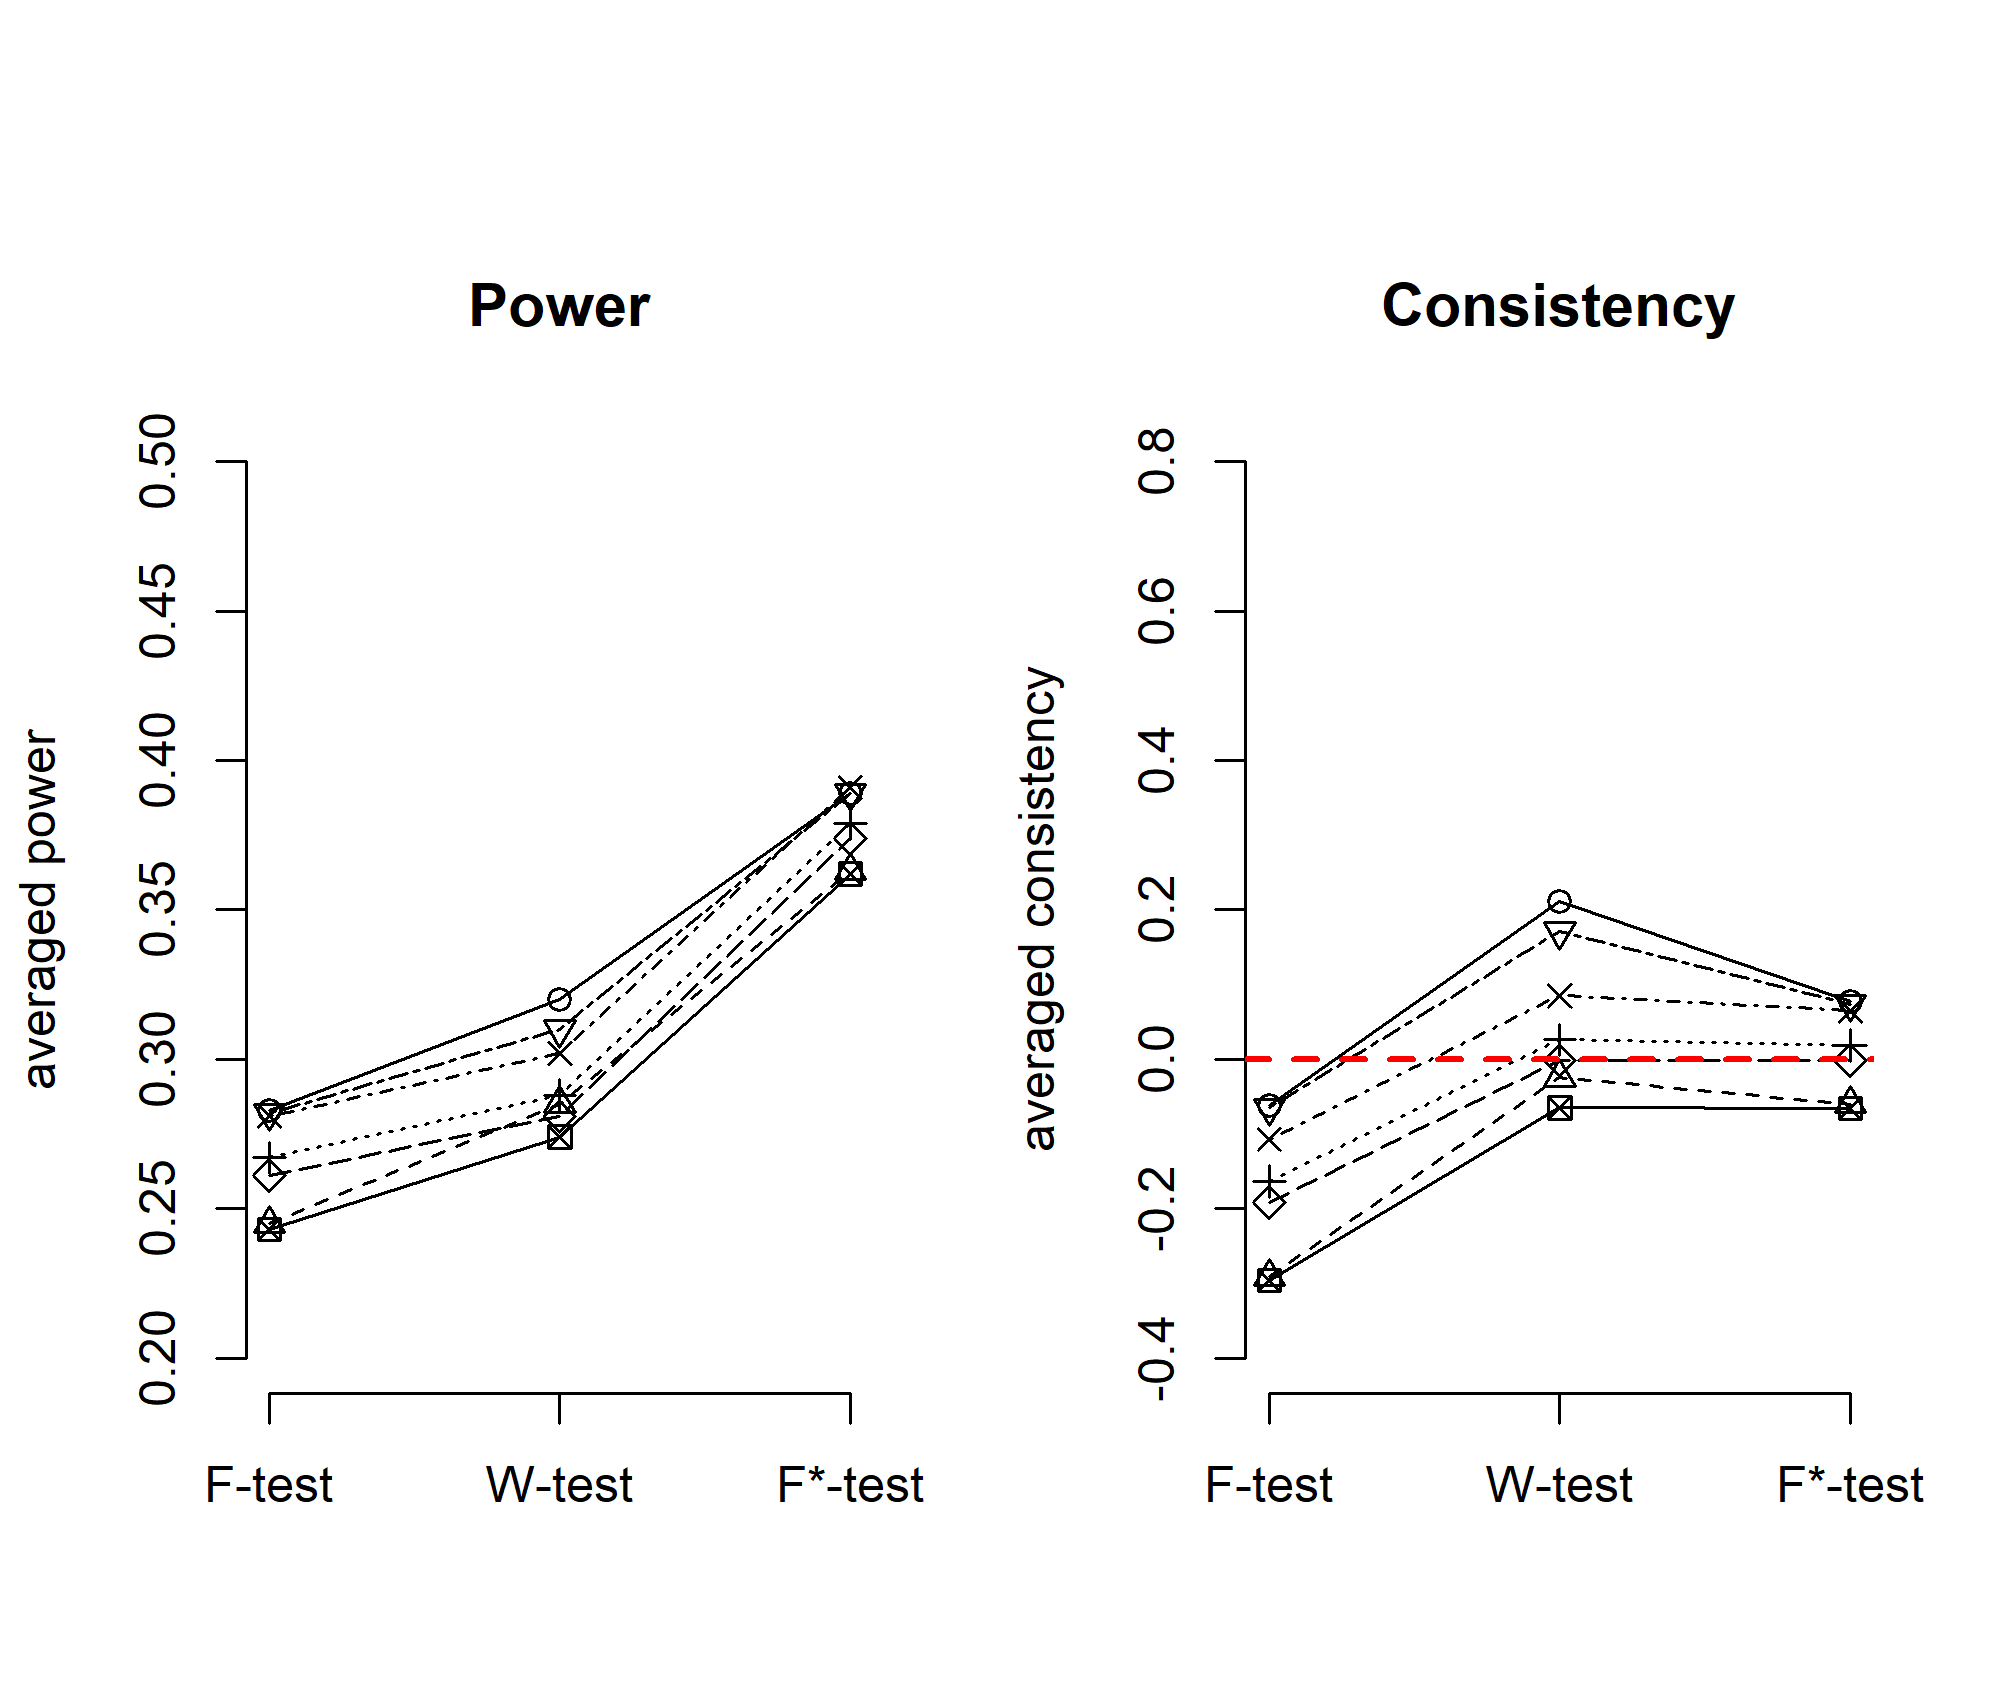
\includegraphics[width=400px]{Rmarkdown folder/Rmarkdown inputs/Fig2f} \caption{Power and consistency of the F-test, W-test and F*-test when there are unequal SDs across groups,negative correlation betwen sample sizes and SDs, and positive correlation between SDs and means (cell f in Table 1)}\label{fig:unnamed-chunk-12}
\end{figure}

\begin{figure}
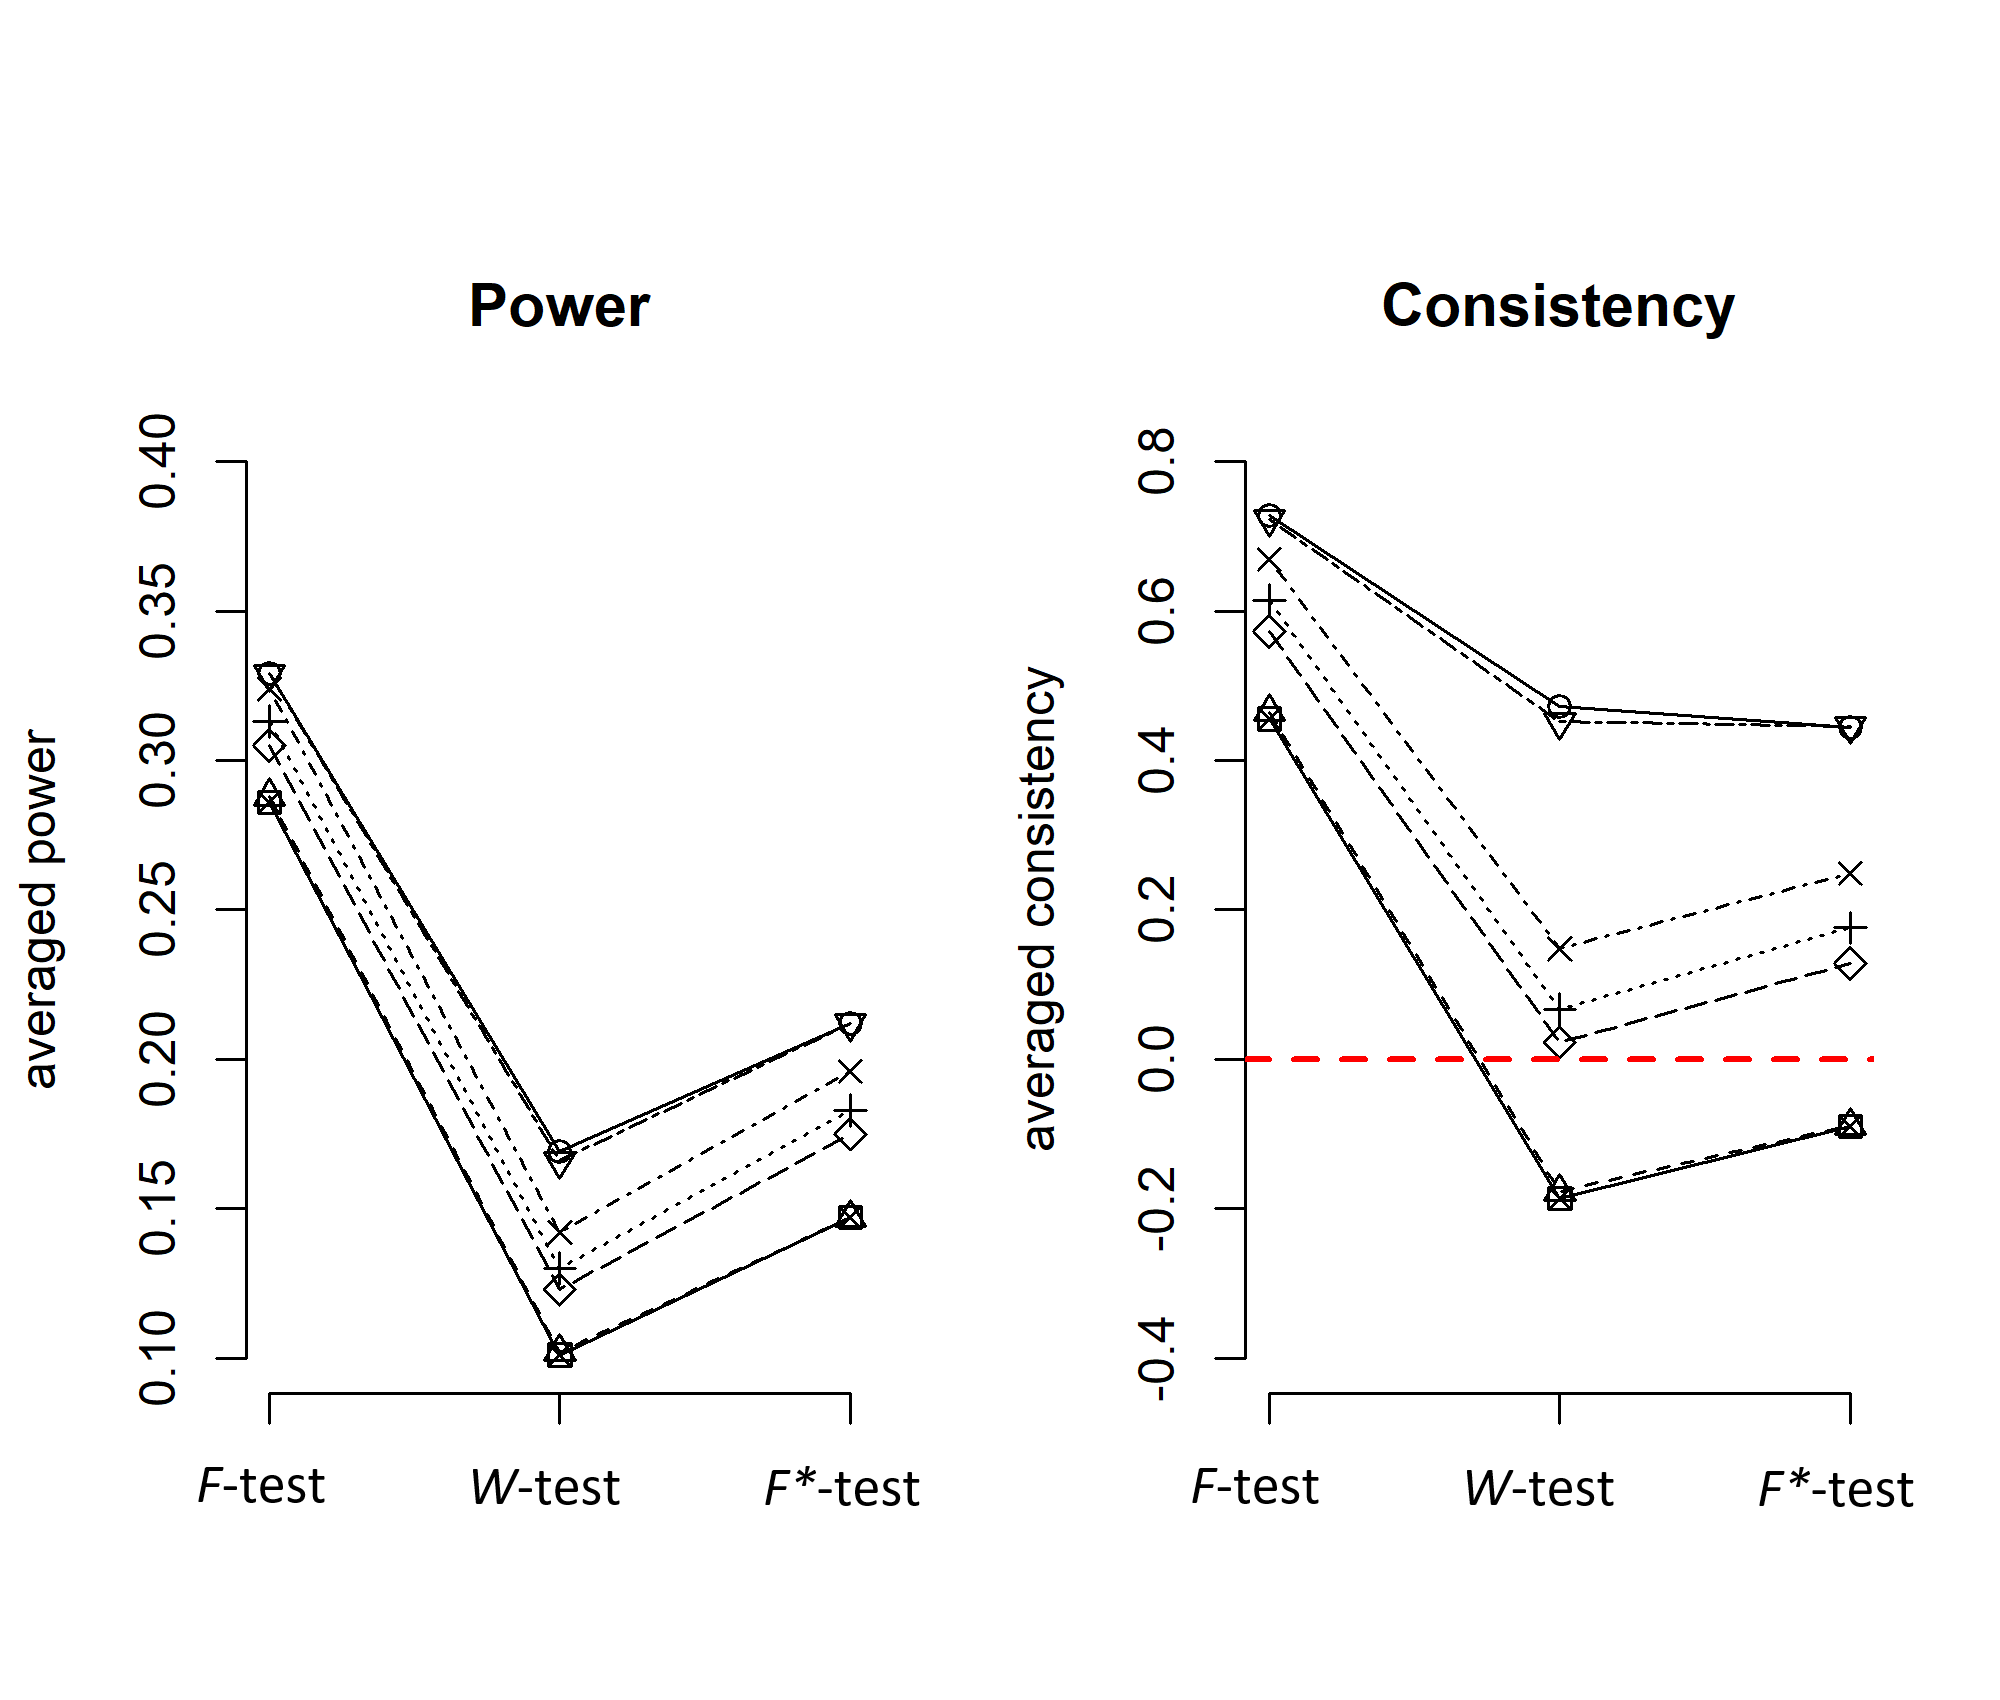
\includegraphics[width=400px]{Rmarkdown folder/Rmarkdown inputs/Fig2g} \caption{Power and consistency of the F-test, W-test and F*-test when there are unequal SDs across groups,negative correlation betwen sample sizes and SDs, and negative correlation between SDs and means (cell h in Table 1)}\label{fig:unnamed-chunk-13}
\end{figure}

\begin{figure}
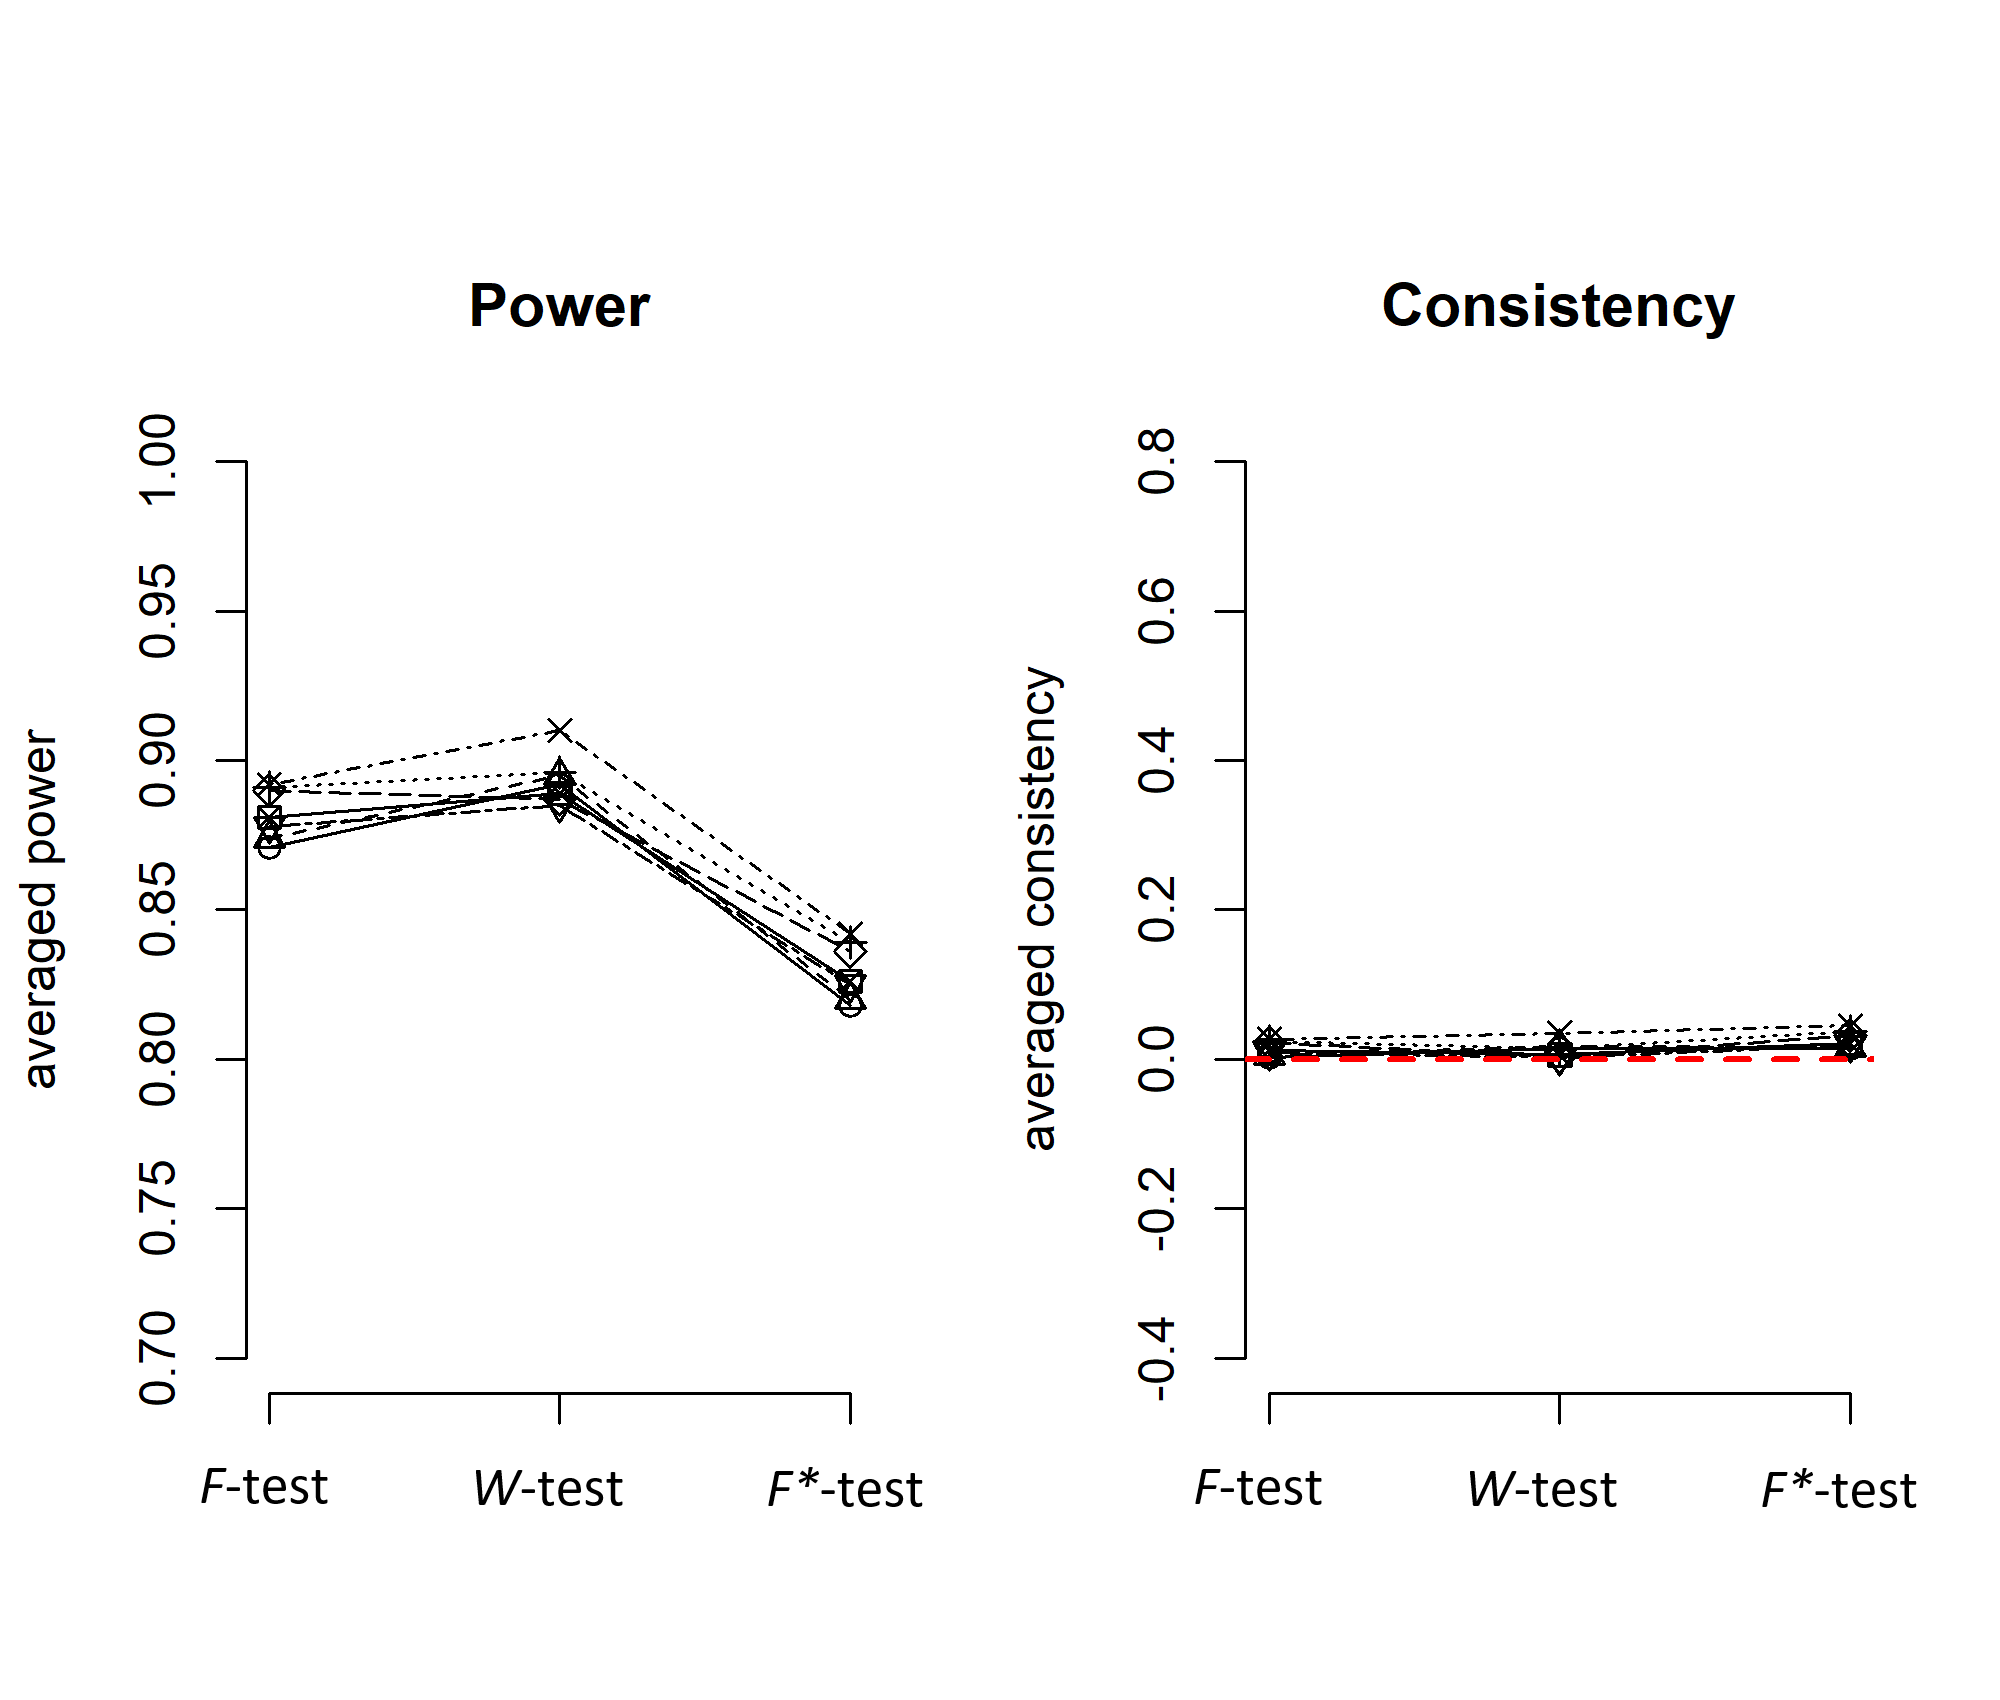
\includegraphics[width=400px]{Rmarkdown folder/Rmarkdown inputs/Fig2h} \caption{Power and consistency of the F-test, W-test and F*-test when there are unequal SDs across groups,positive correlation betwen sample sizes and SDs, and positive correlation between SDs and means (cell e  in Table 1)}\label{fig:unnamed-chunk-14}
\end{figure}

\begin{figure}
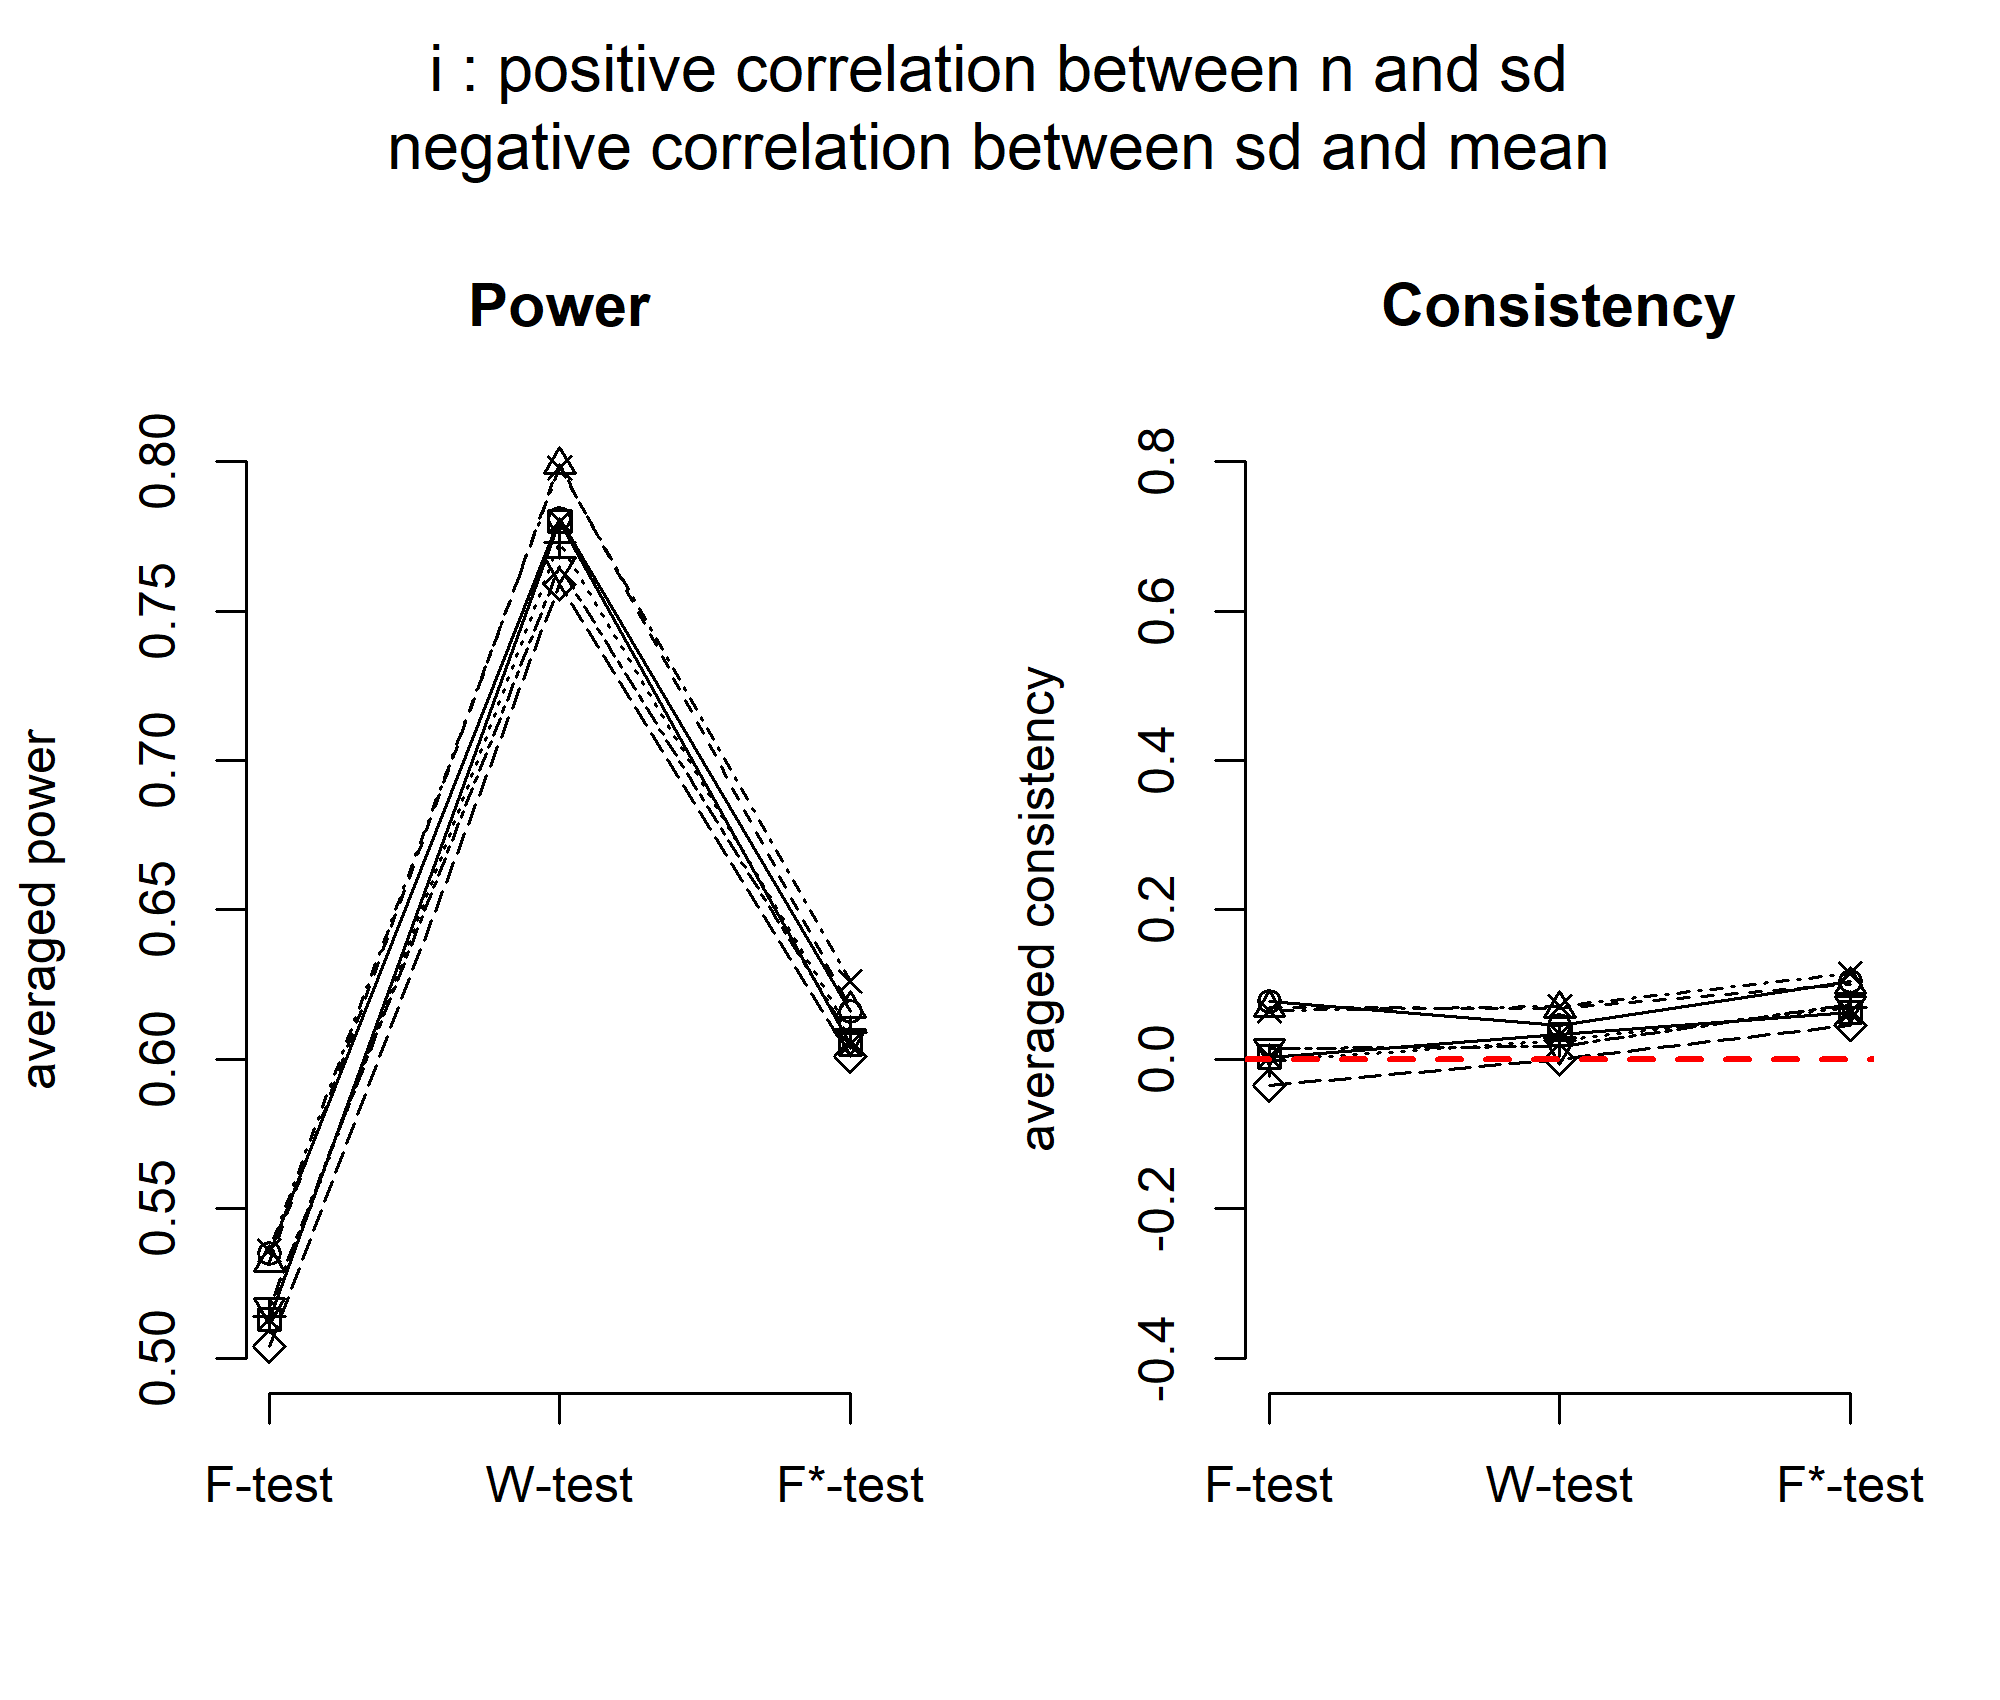
\includegraphics[width=400px]{Rmarkdown folder/Rmarkdown inputs/Fig2i} \caption{Power and consistency of the F-test, W-test and F*-test when there are unequal SDs across groups,positive correlation betwen sample sizes and SDs, and negative correlation between SDs and means (cell i  in Table 1)}\label{fig:unnamed-chunk-15}
\end{figure}

In Figures 7, 8 and 9 (cells a, b, and c in Table 1), the population variance is equal between all groups, meaning that the homoscedasticity assumption is met. When distributions are normal, the \emph{W}-test is slightly less powerful than the \emph{F}-test and \emph{F*}-test, even through differences are very small. With all other distributions, the \emph{W}-test is generally more powerful than the \emph{F*}-test and \emph{F}-test, even with heavy-tailed distributions, which is in contrast with previous findings (Wilcox, 1998). Wilcox (1998) concluded that there is a loss of power when means from heavy-tailed distributions (e.g.~double exponential or a mixed normal distribution) are compared to means from normal distributions. This finding is based on the argument that heavy-tailed distributions are associated with bigger standard deviations than normal distributions, and that the effect size for such distributions is therefore smaller (Wilcox, 2011). However, this conclusion is based on a common conflation of kurtosis and the standard deviation, which are completely independent (DeCarlo, 1997). One can find distributions that have similar \emph{SD} but different kurtosis (see Appendix 2). However, while the \emph{W}-test is more powerful than the \emph{F}-test and the \emph{F*}-test in many situations,it is a bit less consistent with theoretical expectations than both other tests in the sense that the \emph{W}-test is generally more powerful than expected (especially with high kurtosis, or when asymmetries go in opposite directions). This is due to the fact that the \emph{W}-test is more impacted by the distribution shape, in line with observations by Harwell et al. (1992). Note that differences between \emph{W}-test and other tests, in terms of consistency, are very small.

In Figures 10 to 15 (cells d to i in Table 1), the population variance is unequal between groups, meaning that the homoscedasticity assumption is not met. When sample sizes are equal across groups (Figures 10 and 11), the \emph{F}-test and the \emph{F*}-tests are equally powerful, and have the same consistency, whatever the correlation between the \emph{SD} and the mean. On the other hand, the power of the \emph{W}-test depends on the correlation between the \emph{SD} and the mean (in line with Liu, 2015). When the group with the largest mean has the largest variance (Figure 10), the largest deviation between group means and the general mean is given less weight, and as a consequence the \emph{W}-test is less powerful than both other tests. At the same time, the test is slightly less consistent than both other tests. When the group with the largest mean has the smallest variance (Figure 11), the largest deviation between group means and the general mean is given more weight, and therefore the \emph{W}-test is more powerful than both other tests. The test is also slightly more consistent than both other tests.

When sample sizes are unequal across groups, the power of the \emph{F*}-test and the \emph{F}-test are a function of the correlation between sample sizes and \emph{SDs}. When there is a negative correlation between sample sizes and \emph{SDs} (Figures 12 and 13), the \emph{F}-test is always more powerful than the \emph{F*}-test. Indeed, as was explained in the previous mathematical section, the \emph{F}-test gives more weight to the smallest variance (the statistic is therefore increased) while the \emph{F*}-test gives more weight to the largest variance (the statistic is therefore decreased). Conversely, when there is a positive correlation between sample sizes and \emph{SDs} (Figures 14 and 15), the \emph{F}-test is always more conservative than the F\emph{*}-test, because the \emph{F}-test gives more weight to the largest variance while the \emph{F*}-test gives more weight to the smallest variance.

The power of the \emph{W}-test is not a function of the correlation between sample sizes and \emph{SDs}, but rather a function of the correlation between \emph{SDs} and means. The test is more powerful when there is a negative correlation between \emph{SDs} and means, and less powerful when there is a positive correlation between \emph{SDs} and means. Note that for all tests, the effect of heteroscedasticity is approximately the same regardless of the shape of the distribution. Moreover, there is one constant observation in our simulations: whatever the configuration of the \emph{n}-ratio, the consistency of the three tests is closer to zero when there is a negative correlation between the \emph{SD} and the mean (meaning that the group with the highest mean has the lower variance).

We can draw the following conclusions about the statistical power of the three tests:

\begin{enumerate}
\def\labelenumi{\arabic{enumi})}
\tightlist
\item
  When all assumptions are met, the \emph{W}-test falls slightly behind the \emph{F}-test and the \emph{F*}-test, both in terms of power and consistency.
\item
  When variances are equal between groups and distributions are not normal, the \emph{W}-test is slightly more powerful than both the \emph{F}-test and the \emph{F*}-test, even with heavy-tailed distributions.
\item
  When the assumption of equal variances is violated, the \emph{F}-test is either too liberal or too conservative, depending on the correlation between sample sizes and \emph{SDs}. On the other side, the \emph{W}-test is not influenced by the sample sizes and \emph{SDs} pairing. However, it is influenced by the \emph{SD} and means pairing.
\item
  The last conclusion generally remains true when both assumptions of equal variances and normality are not met.
\end{enumerate}

\hypertarget{recommendations}{%
\section{Recommendations}\label{recommendations}}

Taking both the effects of the assumption violations on the alpha risk and on the power, we recommend to use the \emph{W}-test instead of the \emph{F}-test to compare groups means. The \emph{F}-test and \emph{F}*-test should be avoided, because a) the equal variances assumption is often unrealistic, b) tests of the equal variances assumption will often fail to detect differences when these are present, c) the loss of power when using the \emph{W}-test is very small (and often even negligible), and d) the gain in Type I error control is considerable under a wide range of realistic conditions. Also, we recommend the use of balanced designs (i.e.~same sample sizes in each group) whenever possible. When using the \emph{W}-test, the Type I error rate is a function of criteria such as the skewness of the distributions, and whether skewness is combined with unequal variances and unequal samples sizes between groups. Our simulations show that the Type I error rate control is in general slightly better with balanced designs.

Note that the \emph{W}-test suffers from limitations and cannot be used in all situations. First, as previously mentioned, \emph{W}-test, as all tests based on means, does not allow researchers to compare other relevant parameters of a distribution than the mean. For these reason, we recommend to never neglect the descriptive analysis of the data. A complete description of the shape and characteristics of the data (e.g.~histograms and boxplots) is important. When at least one statistical parameter relating to the shape of the distribution (e.g.~variance, skewness, kurtosis) seems to vary between groups, comparing results of the \emph{W}-test with results of a nonparametric procedure is useful in order to better understand the data. Second, with small sample sizes (i.e.~less than 50 observations per group when comparing at most four groups, 100 observations when comparing more than four groups), the \emph{W}-test will not control Type I error rate when skewness is present and detecting departures for normality is therefore especially important in small samples. Unless you have good reasons to believe that distributions underlying the data have small kurtosis and skewness, we recommend to avoid alternative tests that are not based on means comparison, in favour of alternatives such as the trimmed means test (Erceg-Hurn \& Mirosevich, 2008) \footnote{The null hypothesis of the trimmed means test assumes that trimmed means are the same between groups. A trimmed mean is a mean computed on data after removing the lowest and highest values of the distribution . Trimmed means and means are equal when data are symmetric. On the other hand, when data are asymmetric, trimmed means and means differ.} or nonparametric tests. For more information, see Erceg-Hurn and Mirosevich (2008).

\newpage

\hypertarget{references}{%
\section{References}\label{references}}

\setlength{\parindent}{-0.5in}
\setlength{\leftskip}{0.5in}

\hypertarget{refs}{}
\leavevmode\hypertarget{ref-Adams_et_al_2014}{}%
Adams, B. G., Van de Vijver, F. J., de Bruin, G. P., \& Bueno Torres, C. (2014). Identity in descriptions of others across ethnic groups in south africa. \emph{Journal of Cross-Cultural Psychology}, \emph{45}(9), 1411--1433. doi:\href{https://doi.org/10.1177/0022022114542466}{10.1177/0022022114542466}

\leavevmode\hypertarget{ref-Beilmann_et_al_2014}{}%
Beilmann, M., Mayer, B., Kasearu, K., \& Realo, A. (2014). The relationship between adolescents' social capital and individualism-collectivism in estonia, germany, and russia. \emph{Child Indicators Research}, \emph{7}(3), 589--611. doi:\href{https://doi.org/10.1007/s12187-014-9232-z}{10.1007/s12187-014-9232-z}

\leavevmode\hypertarget{ref-Boneau_1960}{}%
Boneau, C. (1960). The effects of violations of assumptions underlying the t test. \emph{Psychological Bulletin}, \emph{57}(1), 49--64.

\leavevmode\hypertarget{ref-Box_1954}{}%
Box, G. (1954). Some theorems on quadratic forms applied in the study of analysis of variance problems, i. Effect of inequality of variance in the one-way classification. \emph{The Annals of Mathematical Statistics}, \emph{25}(2), 290--302.

\leavevmode\hypertarget{ref-Bradley_1978}{}%
Bradley, J. V. (1978). Robustness? \emph{British Journal of Mathematical and Statistical Psychology}, \emph{31}(2), 144--152. doi:\href{https://doi.org/10.1111/j.2044-8317.1978.tb00581.x}{10.1111/j.2044-8317.1978.tb00581.x}

\leavevmode\hypertarget{ref-Brown_and_Forsythe_1974}{}%
Brown, M. B., \& Forsythe, A. B. (1974). Robust tests for the equality of variances. \emph{Journal of the American Statistical Association}, \emph{69}(346), 364--367. doi:\href{https://doi.org/10.2307/2285659}{10.2307/2285659}

\leavevmode\hypertarget{ref-Bryk_and_Raudenbush_1988}{}%
Bryk, A. S., \& Raudenbush, S. W. (1988). Heterogeneity of variance in experimental studies: A challenge to conventional interpretations. \emph{Psychological Bulletin}, \emph{104}(3), 396--404. doi:\href{https://doi.org/10.1037/0033-2909.104.3.396}{10.1037/0033-2909.104.3.396}

\leavevmode\hypertarget{ref-Cain_et_al_2016}{}%
Cain, M. K., Zhang, Z., \& Yuan, K.-H. (2017). Univariate and multivariate skewness and kurtosis for measuring nonnormality: Prevalence, influence and estimation. \emph{Behavior Research Methods}, \emph{49}(5), 1716--1735. doi:\href{https://doi.org/10.3758/s13428-016-0814-1}{10.3758/s13428-016-0814-1}

\leavevmode\hypertarget{ref-Church_et_al_2012}{}%
Church, A. T., Willmore, S. L., Anderson, A. T., Ochiai, M., Porter, N., Mateo, N. J., \ldots{} Ortiz, F. A. (2012). Cultural differences in implicit theories and self-perceptions of traitedness: Replication and extension with alternative measurement formats and cultural dimensions. \emph{Journal of Cross-Cultural Psychology}, \emph{43}(8), 1268--1296. doi:\href{https://doi.org/10.1177/0022022111428514}{10.1177/0022022111428514}

\leavevmode\hypertarget{ref-Cohen_and_Hill_2007}{}%
Cohen, A. B., \& Hill, P. C. (2007). Religion as culture: Religious individualism and collectivism among american catholics, jews, and protestants. \emph{Journal of Personality}, \emph{75}(4), 709--742. doi:\href{https://doi.org/10.1111/j.1467-6494.2007.00454.x\%20}{10.1111/j.1467-6494.2007.00454.x }

\leavevmode\hypertarget{ref-Cohen_et_al_2013}{}%
Cohen, J., Cohen, P., West, S. G., \& Aiken, L. S. (2013). \emph{Applied multiple regression/correlation analysis for the behavioural sciences} (Erlbaum.). Mahwah, NJ.

\leavevmode\hypertarget{ref-Cumming_2013}{}%
Cumming, G. (2005). \emph{Understanding the new statistics: Effect sizes, confidence intervals, and meta-analysis} (Routledge.). New York, NY.

\leavevmode\hypertarget{ref-David_and_Johnson_1951}{}%
David, F. N., \& Johnson, N. L. (1951). The effect of nonnormality on the power function of the f-test in the analysis of variance. \emph{Biometrika}, \emph{38}(1-2), 43--57. doi:\href{https://doi.org/10.2307/2332316}{10.2307/2332316}

\leavevmode\hypertarget{ref-DeCarlo_1997}{}%
DeCarlo, L. T. (1997). On the meaning and use of kurtosis. \emph{Psychological Methods}, \emph{2}(3), 292--307. doi:\href{https://doi.org/10.1037//1082-989x.2.3.292}{10.1037//1082-989x.2.3.292}

\leavevmode\hypertarget{ref-Delacre_et_al_2017}{}%
Delacre, M., Lakens, D., \& Leys, C. (2017). Why psychologists should by default use welch's t-test instead of student's t-test. \emph{International Review of Social Psychology}, \emph{30}(1), 92--101. doi:\href{https://doi.org/10.5334/irsp.82}{10.5334/irsp.82}

\leavevmode\hypertarget{ref-Erceg-Hurn_Mirosevich_2008}{}%
Erceg-Hurn, D. M., \& Mirosevich, V. M. (2008). Modern robust statistical methods: An easy way to maximize the accuracy and power of your research. \emph{American Psychologist}, \emph{63}(7), 591--601. doi:\href{https://doi.org/10.1037/0003-066X.63.7.591}{10.1037/0003-066X.63.7.591}

\leavevmode\hypertarget{ref-Glass_et_al_1972}{}%
Glass, G. V., Peckham, P. D., \& Sanders, J. R. (1972). Consequences of failure to meet assumptions underlying the fixed effects analyses of variance and covariance. \emph{Review of Educational Research}, \emph{42}(3), 237--288. doi:\href{https://doi.org/10.3102/00346543042003237}{10.3102/00346543042003237}

\leavevmode\hypertarget{ref-Green_et_al_2005}{}%
Green, E. G., Deschamps, J.-C., \& Páez, D. (2005). Variation of individualism and collectivism within and between 20 countries: A typological analysis. \emph{Journal of Cross-Cultural Psychology}, \emph{36}(3), 321--339. doi:\href{https://doi.org/10.1177/0022022104273654}{10.1177/0022022104273654}

\leavevmode\hypertarget{ref-Grey_and_Mathiews_2000}{}%
Grey, S., \& Mathews, A. (2000). Effects of training on interpretation of emotional ambiguity. \emph{The Quarterly Journal of Experimental Psychology}, \emph{53}(4), 1143--1162. doi:\href{https://doi.org/10.1080/713755937}{10.1080/713755937}

\leavevmode\hypertarget{ref-Grissom_2000}{}%
Grissom, R. (2000). Heterogeneity of variance in clinical data. \emph{Journal of Consulting and Clinical Psychology}, \emph{68}(1), 155--165. doi:\href{https://doi.org/10.1037//0022-006x.68.1.155}{10.1037//0022-006x.68.1.155}

\leavevmode\hypertarget{ref-Haar_et_al_2014}{}%
Haar, J. M., Russo, M., Suñe, A., \& Ollier-Malaterre, A. (2014). Outcomes of work-life balance on job satisfaction, life satisfaction and mental health: A study across seven cultures. \emph{Journal of Vocational Behavior}, \emph{85}(3), 361--373. doi:\href{https://doi.org/10.1016/j.jvb.2014.08.010}{10.1016/j.jvb.2014.08.010}

\leavevmode\hypertarget{ref-Harwell_et_al_1992}{}%
Harwell, M. R., Rubinstein, E. N., Hayes, W. S., \& Olds, C. C. (1992). Summarizing monte carlo results in methodological research: The one- and two-factor fixed effects anova cases. \emph{Journal of Educational Statistics}, \emph{17}(4), 315--339.

\leavevmode\hypertarget{ref-Henrich_et_al_2010}{}%
Henrich, J., Heine, S. J., \& Norenzayan, A. (2010). Most people are not weird. \emph{Nature}, \emph{466}, 29--29. doi:\href{https://doi.org/10.1038/466029a\%20}{10.1038/466029a }

\leavevmode\hypertarget{ref-Heun_et_al_1999}{}%
Heun, R., Burkart, M., Maier, W., \& Bech, P. (1999). Internal and external validity of the who well-being scale in the elderly general population. \emph{Acta Psychiatrica Scandinavica}, \emph{99}(3), 171--178. doi:\href{https://doi.org/10.1111/j.1600-0447.1999.tb00973.x\%20}{10.1111/j.1600-0447.1999.tb00973.x }

\leavevmode\hypertarget{ref-Hoekstra_et_al_2012}{}%
Hoekstra, R., Kiers, H. A., \& Johnson, A. (2012). Are assumptions of well-known statistical techniques checked, and why (not)? \emph{Frontiers in Psychology}, \emph{3}(137), 1--9. doi:\href{https://doi.org/10.3389/fpsyg.2012.00137}{10.3389/fpsyg.2012.00137}

\leavevmode\hypertarget{ref-Hsu_and_Feldt_1969}{}%
Hsu, T.-C., \& Feldt, L. S. (1969). The effect of limitations on the number of criterion score values on the significance level of the f-test. \emph{American Educational Research Journal}, \emph{6}(4), 515--527. doi:\href{https://doi.org/10.3102/00028312006004515}{10.3102/00028312006004515}

\leavevmode\hypertarget{ref-Keppel_and_Wickens_2004}{}%
Keppel, G., \& Wickens, T. D. (2004). \emph{Design and analysis: A researcher's handbook} (Prentice Hall.). Upper Saddle River , New Jersey.

\leavevmode\hypertarget{ref-Keselman_et_al_1998}{}%
Keselman, H., Huberty, C. J., Lix, L. M., Olejnik, S., Cribbie, R. A., Donahue, B., \ldots{} Levin, J. R. (1998). Statistical practices of educational researchers: An analysis of their anova, manova, and ancova analy. \emph{Review of Educational Research}, \emph{68}(3), 350--386.

\leavevmode\hypertarget{ref-Koeser_and_Sczesny_2014}{}%
Koeser, S., \& Sczesny, S. (2014). Promoting gender-fair language: The impact of arguments on language use, attitudes, and cognitions. \emph{Journal of Language and Social Psychology}, \emph{33}(5), 548--560. doi:\href{https://doi.org/10.1177/0261927x14541280}{10.1177/0261927x14541280}

\leavevmode\hypertarget{ref-Liu_2015}{}%
Liu, H. (2015). \emph{Comparing welch anova, a kruskal-wallis test, and traditional anova in case of heterogeneity of variance} (PhD thesis). Virginia Commonwealth University.

\leavevmode\hypertarget{ref-Lix_Keselman_Keselman_1996}{}%
Lix, L. M., Keselman, J. C., \& Keselman, H. (1996). Consequences of assumption violations revisited: A quantitative review of alternatives to the one-way analysis of variance *f* test. \emph{Review of Educational Research}, \emph{66}(4), 579--619. doi:\href{https://doi.org/10.3102/00346543066004579}{10.3102/00346543066004579}

\leavevmode\hypertarget{ref-Micceri_1989}{}%
Micceri, T. (1989). The unicorn, the normal curve, and other improbable creatures. \emph{Psychological Bulletin}, \emph{105}(1), 156--166. doi:\href{https://doi.org/10.1037/0033-2909.105.1.156}{10.1037/0033-2909.105.1.156}

\leavevmode\hypertarget{ref-Montoya_Briggs_2013}{}%
Montoya, D. Y., \& Briggs, E. (2013). Shared ethnicity effects on service encounters: A study across three us subcultures. \emph{Journal of Business Research}, \emph{66}(3), 314--320. doi:\href{https://doi.org/10.1016/j.jbusres.2011.08.011}{10.1016/j.jbusres.2011.08.011}

\leavevmode\hypertarget{ref-Nimon_2012}{}%
Nimon, K. F. (2012). Statistical assumptions of substantive analyses across the general linear model: A mini-review. \emph{Frontiers in Psychology}, \emph{3}(322), 1--5. doi:\href{https://doi.org/10.3389/fpsyg.2012.00322}{10.3389/fpsyg.2012.00322}

\leavevmode\hypertarget{ref-Overall_et_al_1995}{}%
Overall, J. E., Atlas, R. S., \& Gibson, J. M. (1995). Tests that are robust against variance heterogeneity in k x 2 designs with unequal cell frequencies. \emph{Psychological Reports}, \emph{76}(3), 1011--1017. doi:\href{https://doi.org/10.2466/pr0.1995.76.3.1011}{10.2466/pr0.1995.76.3.1011}

\leavevmode\hypertarget{ref-Quensel_1947}{}%
Quensel, C.-E. (1947). The validity of the *z*-criterion when the variates are taken from different normal populations. \emph{Scandinavian Actuarial Journal}, \emph{30}(1), 44--55. doi:\href{https://doi.org/10.1080/03461238.1947.10419648}{10.1080/03461238.1947.10419648}

\leavevmode\hypertarget{ref-Ratcliff_1979}{}%
Ratcliff, R. (1979). Group reaction time distributions and an analysis of distribution statistics. \emph{Psychological Bulletin}, \emph{86}(3), 446--461. doi:\href{https://doi.org/10.1037/0033-2909.86.3.446}{10.1037/0033-2909.86.3.446}

\leavevmode\hypertarget{ref-Schneider_and_Penfield_1997}{}%
Schneider, P. J., \& Penfield, D. A. (1997). Alexander and govern's approximations: Providing an alternative to anova under variance heterogeneity. \emph{The Journal of Experimental Education}, \emph{65}(3), 271--286. doi:\href{https://doi.org/10.1080/00220973.1997.9943459}{10.1080/00220973.1997.9943459}

\leavevmode\hypertarget{ref-Srivastava_1959}{}%
Srivastava, A. B. L. (1959). Effects of non-normality on the power of the analysis of variance test. \emph{Biometrika}, \emph{46}(1-2), 114--122. doi:\href{https://doi.org/10.2307/2332813}{10.2307/2332813}

\leavevmode\hypertarget{ref-Tiku_1971}{}%
Tiku, M. (1971). Power function of the f-test under non-normal situations. \emph{Journal of the American Statistical Association}, \emph{66}, 913--916. doi:\href{https://doi.org/10.1080/01621459.1971.10482371}{10.1080/01621459.1971.10482371}

\leavevmode\hypertarget{ref-Tomarken_and_Serlin_1986}{}%
Tomarken, A. J., \& Serlin, R. C. (1986). Comparison of anova alternatives under variance heterogeneity and specific noncentrality structures. \emph{Psychological Bulletin}, \emph{99}(1), 90--99. doi:\href{https://doi.org/10.1037//0033-2909.99.1.90}{10.1037//0033-2909.99.1.90}

\leavevmode\hypertarget{ref-Wasserman_and_Weseley_2009}{}%
Wasserman, B. D., \& Weseley, A. J. (2009). ?'Qué? Quoi? Do languages with grammatical gender promote sexist attitudes? \emph{Sex Roles}, \emph{61}, 634--643. doi:\href{https://doi.org/10.1007/s11199-009-9696-3}{10.1007/s11199-009-9696-3}

\leavevmode\hypertarget{ref-Westfall_2014}{}%
Westfall, P. H. (2014). Kurtosis as peakedness, 1905-2014. R.I.P. \emph{The American Statistician}, \emph{68}(3), 191--195. doi:\href{https://doi.org/10.1080/00031305.2014.917055}{10.1080/00031305.2014.917055}

\leavevmode\hypertarget{ref-Wilcox_1998}{}%
Wilcox, R. R. (1998). How many discoveries have been lost by ignoring modern statistical methods? \emph{American Psychologist}, \emph{53}(3), 300--314. doi:\href{https://doi.org/10.1037/0003-066x.53.3.300}{10.1037/0003-066x.53.3.300}

\leavevmode\hypertarget{ref-Wilcox_2005}{}%
Wilcox, R. R. (2005). Comparing medians: An overview plus new results on dealing with heavy-tailed distributions. \emph{The Journal of Experimental Education}, \emph{73}(3), 249--263. doi:\href{https://doi.org/10.3200/JEXE.73.3.249-263}{10.3200/JEXE.73.3.249-263}

\leavevmode\hypertarget{ref-Wilcox_2011}{}%
Wilcox, R. R. (2011). \emph{Introduction to robust estimation and hypothesis testing} (Academic Press.). Cambridge, Massachusetts, US.

\leavevmode\hypertarget{ref-Yuan_et_al_2004}{}%
Yuan, K.-H., Bentler, P. M., \& Chan, W. (2004). Structural equation modeling with heavy tailed distributions. \emph{Psychometrika}, \emph{69}(3), 421--436. doi:\href{https://doi.org/10.1007/bf02295644}{10.1007/bf02295644}

\clearpage
\makeatletter
\efloat@restorefloats
\makeatother


\begin{appendix}
\section{}
\setlength{\parindent}{0.0in}
\setlength{\leftskip}{0.0in}

\hypertarget{appendix-1-the-mathematical-development-of-the-f-test-w-test-and-f-test-numerical-example}{%
\subsection{\texorpdfstring{Appendix 1: The Mathematical Development of
the \emph{F}-test, \emph{W}-test, and \emph{F}*-test: Numerical
Example}{Appendix 1: The Mathematical Development of the F-test, W-test, and F*-test: Numerical Example}}\label{appendix-1-the-mathematical-development-of-the-f-test-w-test-and-f-test-numerical-example}}

A summary is presented in Table A1. The complete example is available on
Github. The DV is a score that can vary from 0 to 40. The IV is a
three-level factor A (levels = \(A_1\), \(A_2\) and \(A_3\)).

\begin{figure}
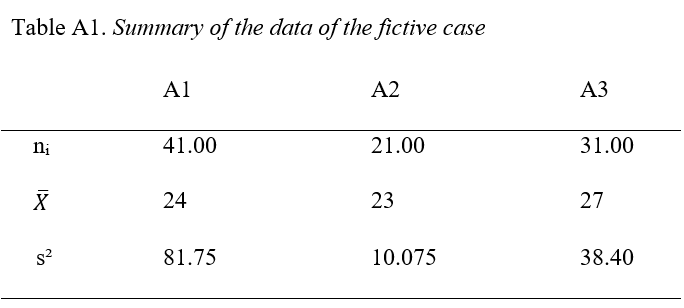
\includegraphics[width=1\linewidth]{Rmarkdown folder/Rmarkdown inputs/TableA1} \end{figure}

The global mean (i.e.~the mean of the global dataset) is a weighted mean
of the group means:

\[\frac{(41*24)+(21*23)+(31*27)}{41+21+31}=\frac{2304}{93} \approx 24.77\]

The \emph{F}-test statistic and degrees of freedom are computed by
applying formulas (1), (2) and (3):

\[
F=\frac{\frac{1}{3-1}[41*(24-\frac{2304}{93})^2+21*(23-\frac{2304}{93})^2+31*(27-\frac{2304}{93})^2]}
{\frac{1}{93-3}[(41-1)*81.75+(21-1)*10.07+(31-1)*38.40]} \approx 2.38
\]

\[
df_n=3-1=2
\]

\[
df_d=93-3=90
\]

The \emph{F}*-test and his degrees of freedom are computed by applying
formulas 4, 5 and 6:

\[
F^*=\frac{41*(24-\frac{2304}{93})^2+21*(23-\frac{2304}{93})^2+31*(27-\frac{2304}{93})^2}{(1-\frac{41}{93})*81.75+(1-\frac{21}{93})*10.07+(1-\frac{31}{93})*38.40} \approx 3.09
\]

\[
df_n=3-1=2
\]

\[
df_d=\frac{1}{\frac{(\frac{(1-\frac{41}{93})*81.75}{\sum_{j=1}^k(1-\frac{n_j}{N})s_j^2})^2}{41-1}+\frac{(\frac{(1-\frac{21}{93})*10.07}{\sum_{j=1}^k(1-\frac{n_j}{N})s_j^2})^2}{21-1}+\frac{(\frac{(1-\frac{31}{93})*38.40}{\sum_{j=1}^k(1-\frac{n_j}{N})s_j^2})^2}{31-1}} \approx 81.15
\]

\[ Where \sum_{j=1}^k(1-\frac{n_j}{N})*s_j^2 \approx 79.11\]

Finally, the \emph{W}-test and his degrees of freedom are computed in
applying formulas 7, 8 and 9:

\[
W=\frac{\frac{1}{3-1}[\frac{41}{81.75}(24-\bar{X'})^2+\frac{21}{10.07}(23-\bar{X'})^2+\frac{31}{38.40}(27-\bar{X'})^2]}
{\frac{2(3-2)}{3^2-1}[(\frac{1}{41-1})(1-\frac{\frac{41}{81.75}}{w})^2+(\frac{1}{21-1})(1-\frac{\frac{21}{10.07}}{w})^2+(\frac{1}{31-1})(1-\frac{\frac{31}{38.40}}{w})^2]+1} \approx 4.61
\]

Where:

\(w=\sum_{j=1}^k w_j \approx 3.39\)

\(\bar{X'}=\frac{\sum_{j=1}^k (w_j\bar{x_j})}{w} \approx 24.10\)

\[
df_n=3-1
\]

\[
df_d=\frac{3^2-1}{3[\frac{(1-\frac{w_j}{w})^2}{41-1}+\frac{(1-\frac{w_j}{w})^2}{21-1}+\frac{(1-\frac{w_j}{w})^2}{31-1}]} \approx 59.32
\]

One should notice that in this example, the biggest sample size has the
biggest variance. As previously mentioned, it means that the
\emph{F}-test will be too conservative, because the \emph{F} value
decreases. The \emph{F}*-test will also be a little too conservative,
even if the test is less affected than the \emph{F}-test. As a
consequence: \emph{W} \textgreater{} \emph{F}* \textgreater{} \emph{F}.

\hypertarget{appendix-2-justification-for-the-choice-of-distributions-in-simulations}{%
\subsection{Appendix 2: Justification for the choice of distributions in
simulations}\label{appendix-2-justification-for-the-choice-of-distributions-in-simulations}}

The set of simulations described in the article was repeated for 7
distributions. We used R commands to generate data from different
distributions:

\begin{itemize}
\item
\emph{k} normal distributions (Figure A1): in order to assess the Type
I error rate and power of the different tests under the assumption of
normality, data were generated by means of the function ``rnorm''
(from the package ``stats''; ``R: The Normal Distribution,'' 2016).
\item
\emph{k} double exponential distributions (Figure A2): In order to
assess the impact of high kurtosis on the Type I error rate and power
of all tests, data were generated by means of the function
``rdoublex'' (from the package ``smoothmest''; ``R: The double
exponential (Laplace) distribution,'' 2012).
\item
\emph{k} mixed normal distributions (Figure A3): In order to assess
the impact of extremely high kurtosis on the Type I error rate and
power of all tests, regardless of variance, data were generated by
means of the function ``rmixnorm'' (from the package ``bda''; Wang \&
Wang, 2015).
\item
\emph{k} normal right skewed distributions (Figure A4): In order to
assess the impact of moderate skewness on the Type I error rate and
power, data were generated by means of the function ``rsnorm'' (from
the package ``fGarch''; ``R: Skew Normal Distribution,'' 2017). The
normal skewed distribution was chosen because it is the only skewed
distribution where the standard deviation ratio can vary without
having an impact on skewness.
\item
\emph{k}-1 normal left skewed distributions (Figure A5) and 1 normal
right skewed distribution (Figure A2.4): In order to assess the impact
of unequal shapes, in terms of skewness, on the Type I error rate and
power, when data have moderate skewness, data were generated by means
of the functions ``rsnorm'' (from the package ``fGarch''; ``R: Skew
Normal Distribution,'' 2017).
\item
\emph{k}-1 chi-squared distributions with two degrees of freedom (See
Figure A6), and one normal rigt skewed distribution (Figure A2.4): In
order to assess the impact of high asymetry on the Type I error rate
an power, k-1 distributions were generated by means of the functions
``rchisq'' (``R: The (non-central) Chi-squared Distribution,'' 2016).
The last distribution was generated by means of ``rsnorm'' in order to
follow a normal right skewed distribution with a mean of 2 (from the
package ``fGarch''; ``R: Skew Normal Distribution,'' 2017). Because
the chi-squared is non-negative, it is not possible to generate
chi-squared where population SD= 1, 4 or 8 and population mean is the
same than the chi-squared with two degrees of freedom. However, we
wanted to assess the impact of different SD-ratio on Type I error
rate. For these reasons, the last distribution was generated by means
of ``rsnorm'' in order to follow a normal skewed distribution with
positive skewness of +0.99 and mean = 2 (from the package ``fGarch'';
``R: Skew Normal Distribution,'' 2017).
\item
\emph{k}-1 chi-squared distributions with two degrees of freedom (See
Figure A6), and one normal left skewed distribution (Figure A5): In
order to assess the impact of unequal shapes, in terms of skewness, on
Type I error rate and power when distributions have extreme skewness,
k-1 distributions were generated by means of the functions ``rchisq''
(``R: The (non-central) Chi-squared Distribution,'' 2016). The last
distribution was generated by means of ``rsnorm'' in order to follow a
normal right skewed distribution with a mean of 2 (from the package
``fGarch''; ``R: Skew Normal Distribution,'' 2017)
\end{itemize}

\begin{figure}
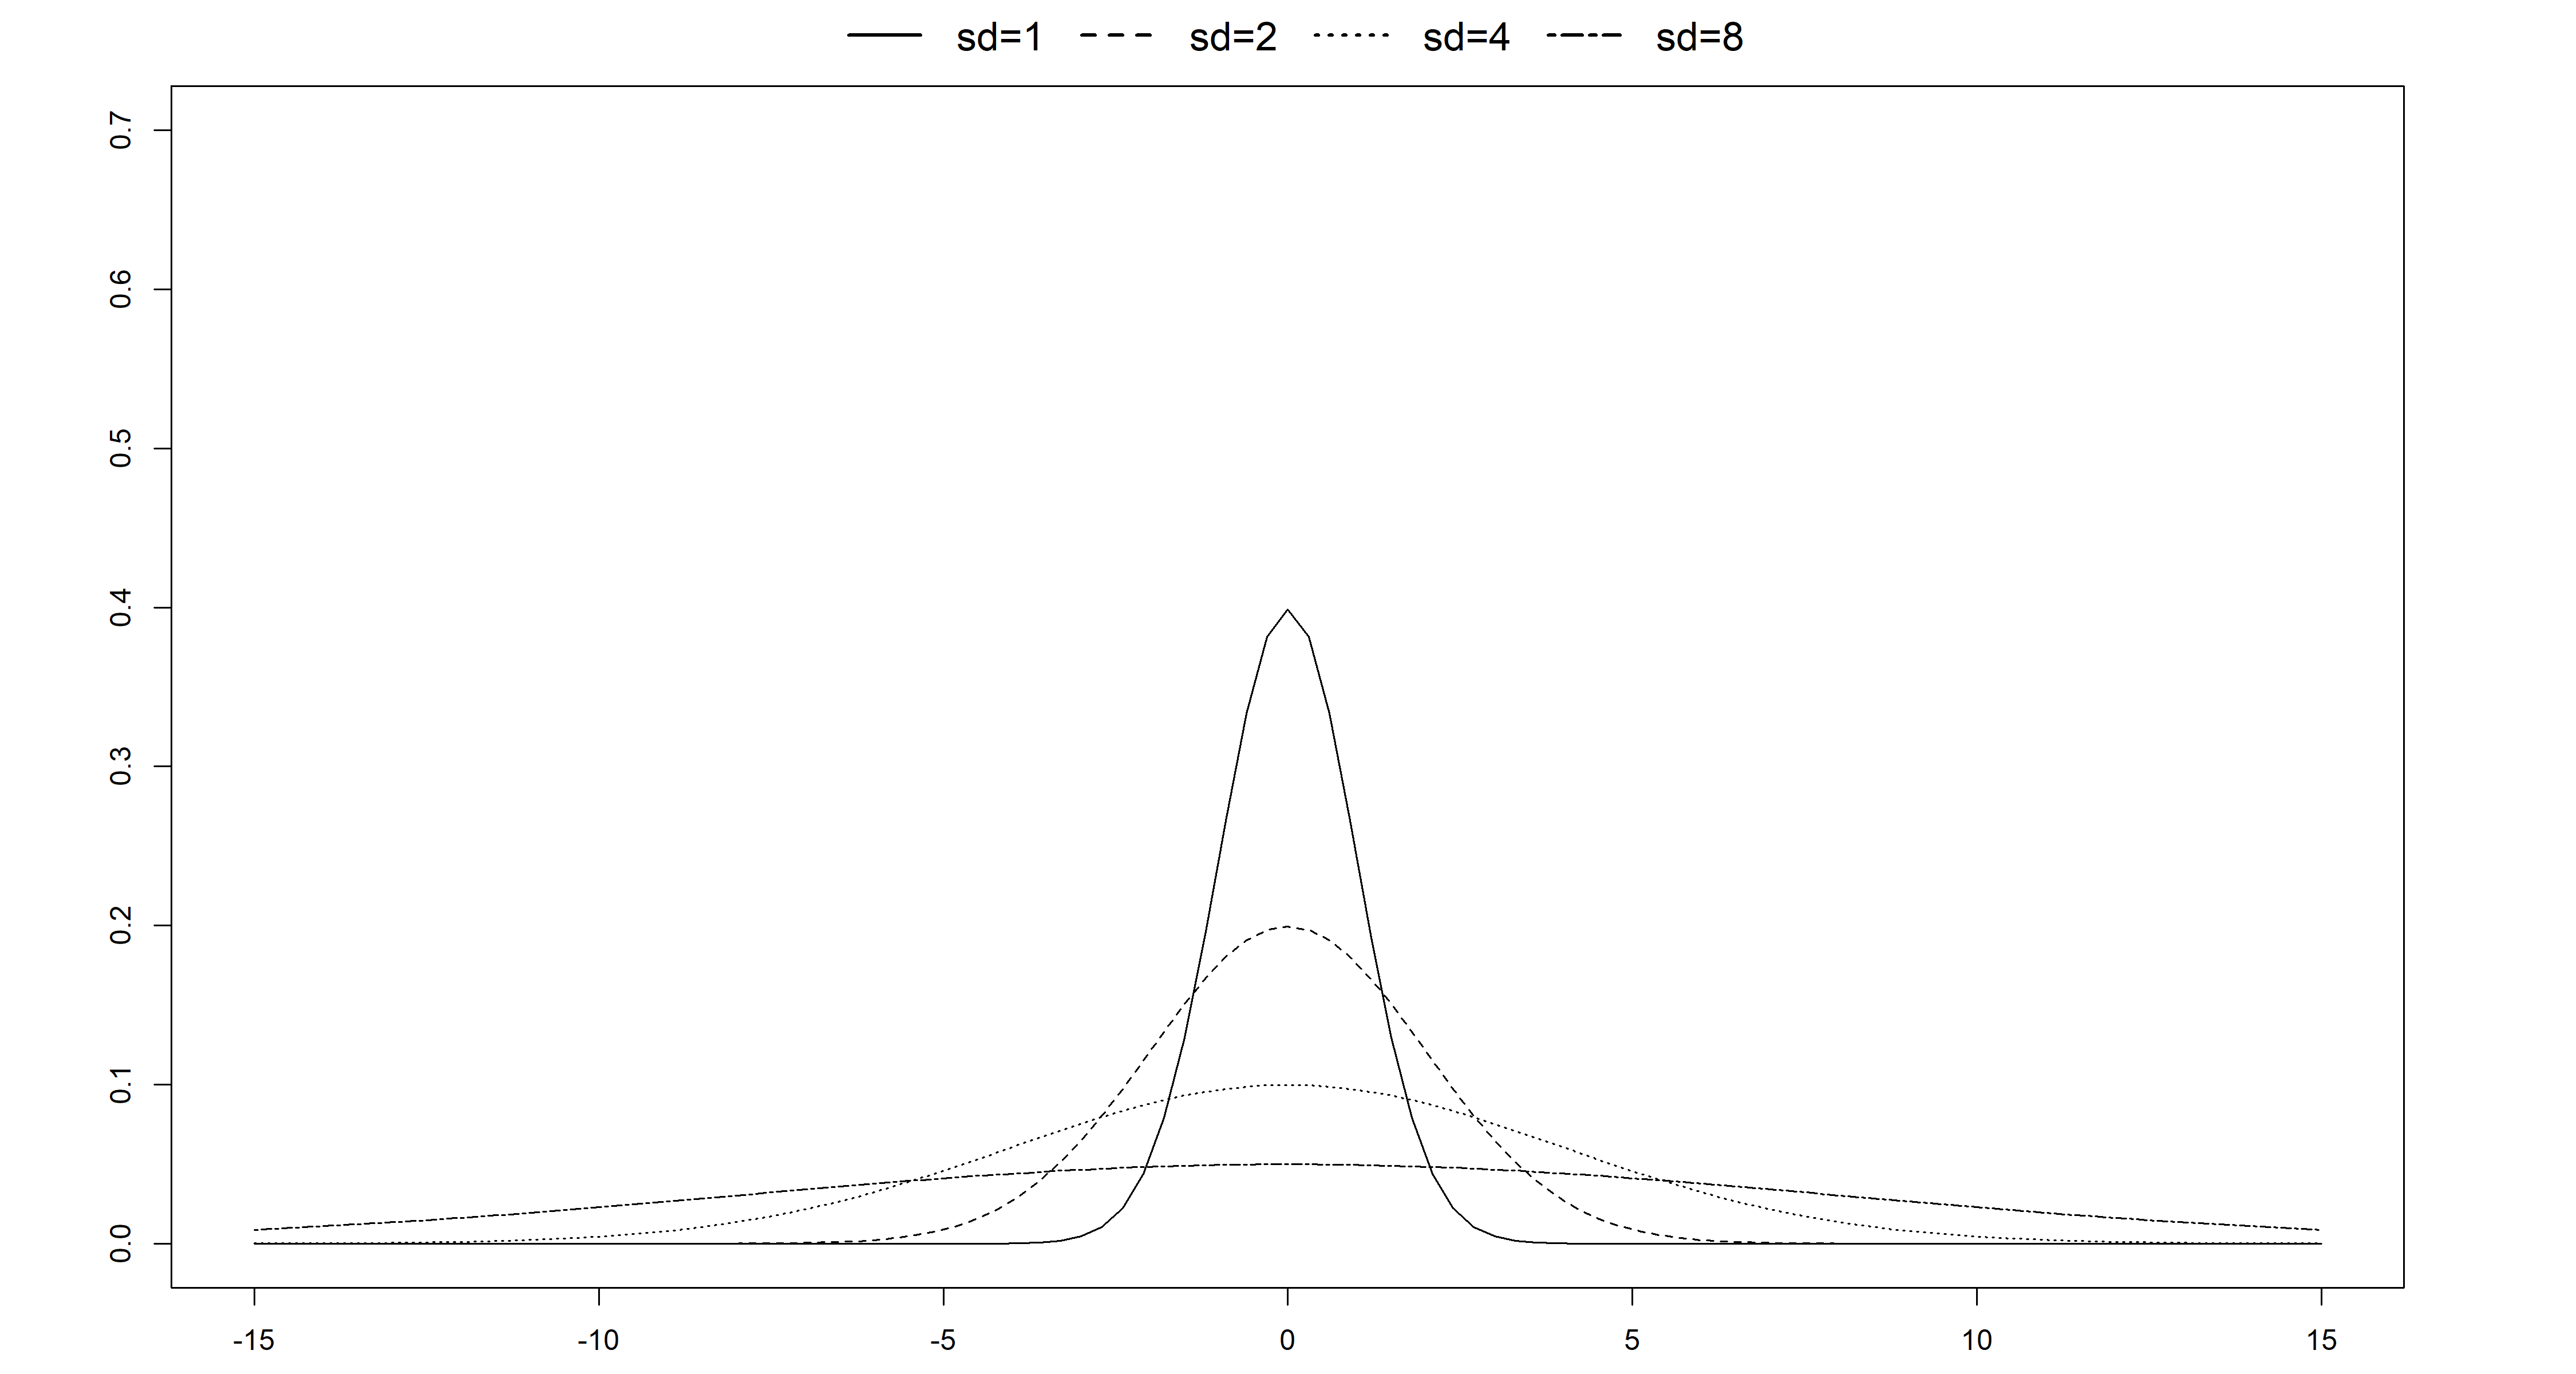
\includegraphics[width=400px]{W-test_files/figure-latex/unnamed-chunk-18-1} \caption{centered normal probability density function, as a function of the population SD}\label{fig:unnamed-chunk-18}
\end{figure}

\begin{figure}
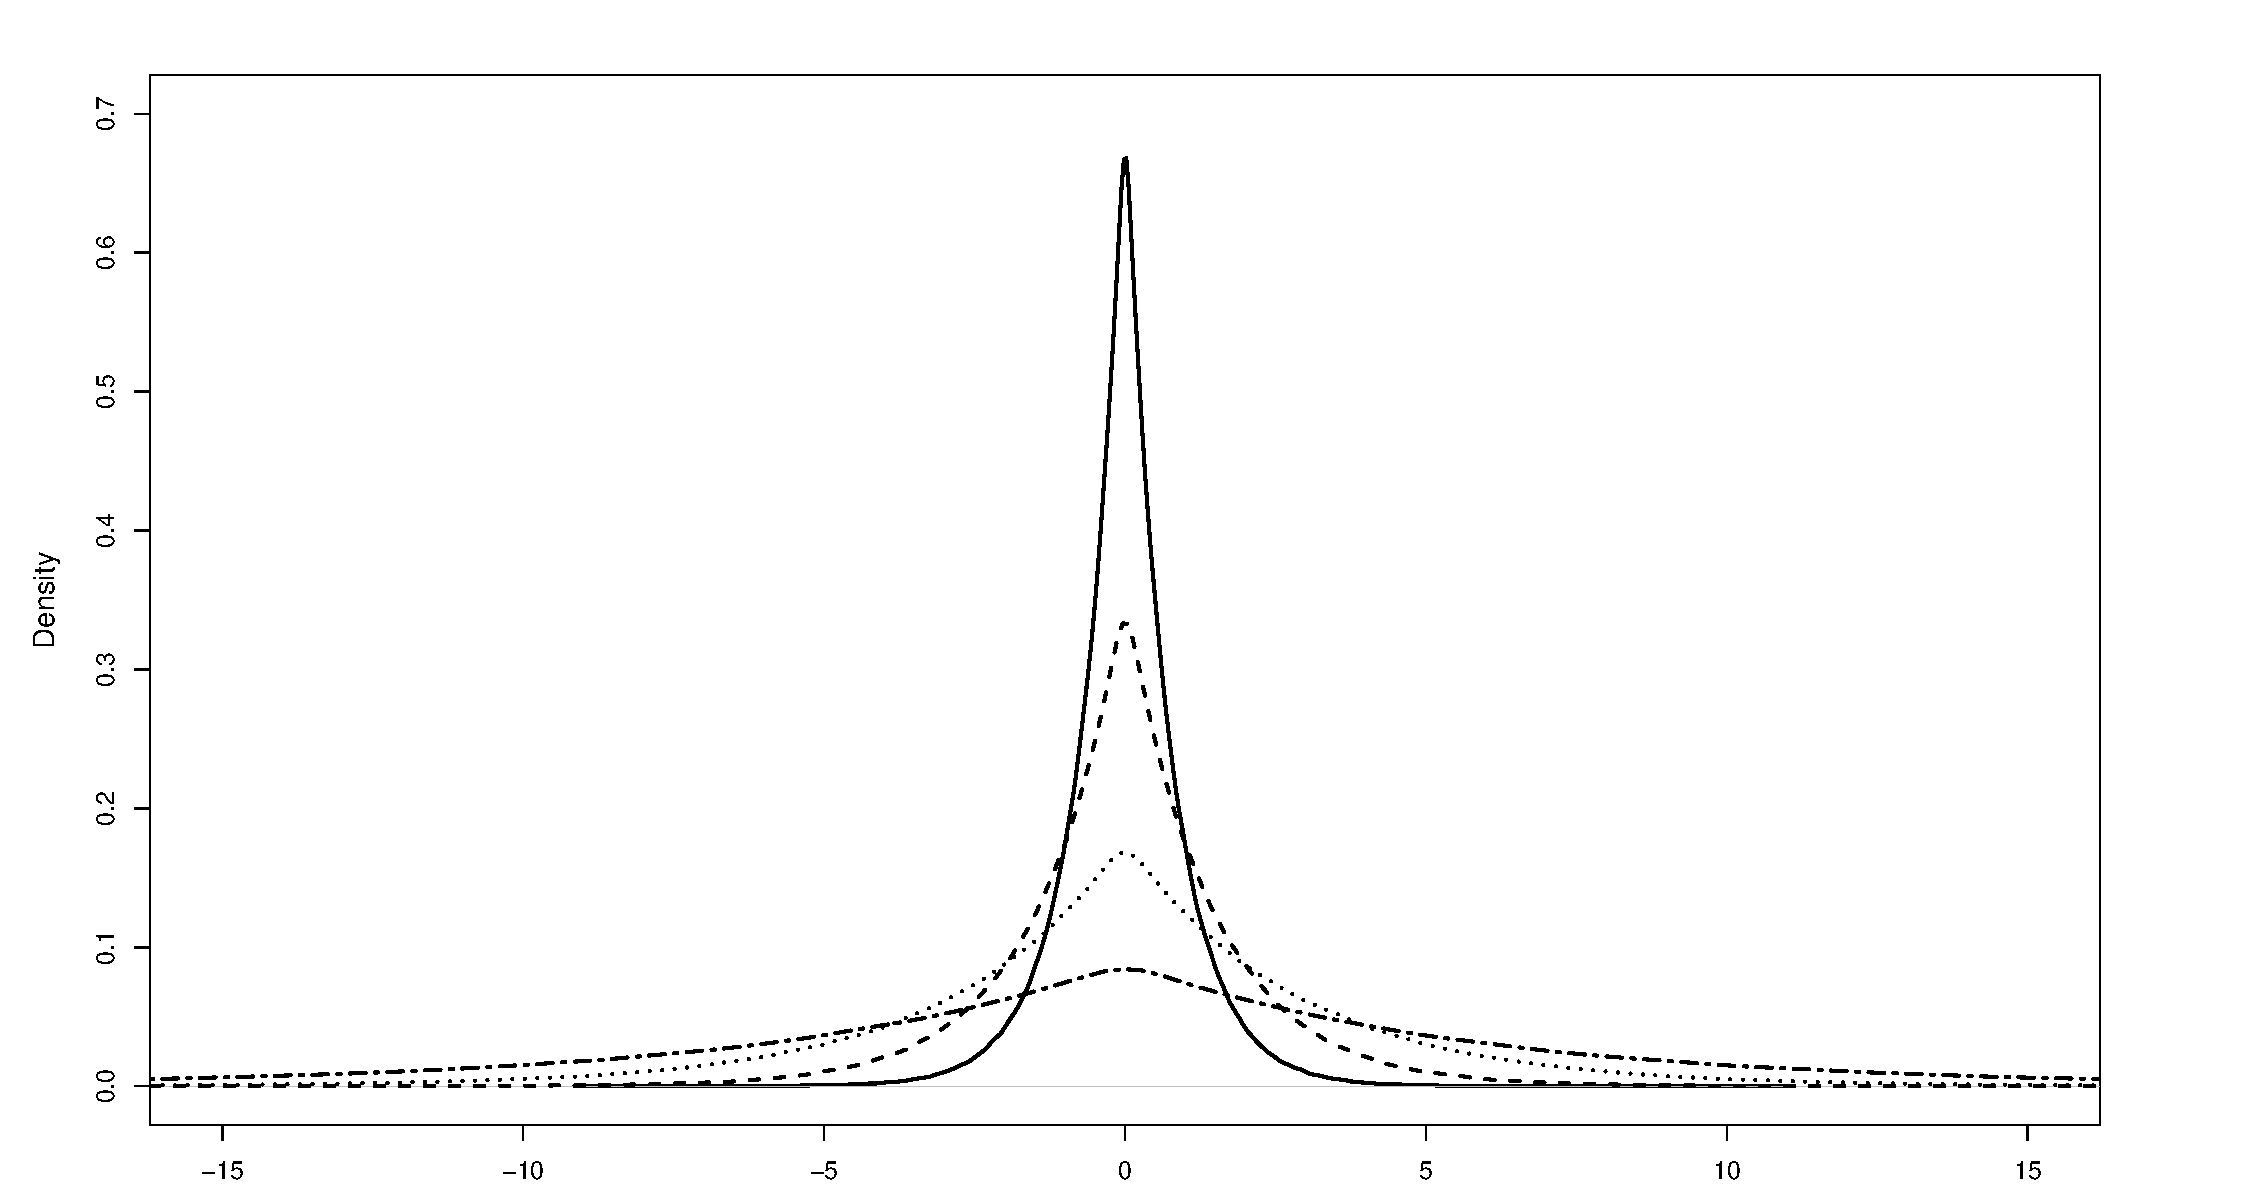
\includegraphics[width=400px]{W-test_files/figure-latex/unnamed-chunk-19-1} \caption{centered double exponential probability density function, as a function of the population SD}\label{fig:unnamed-chunk-19}
\end{figure}

\begin{figure}
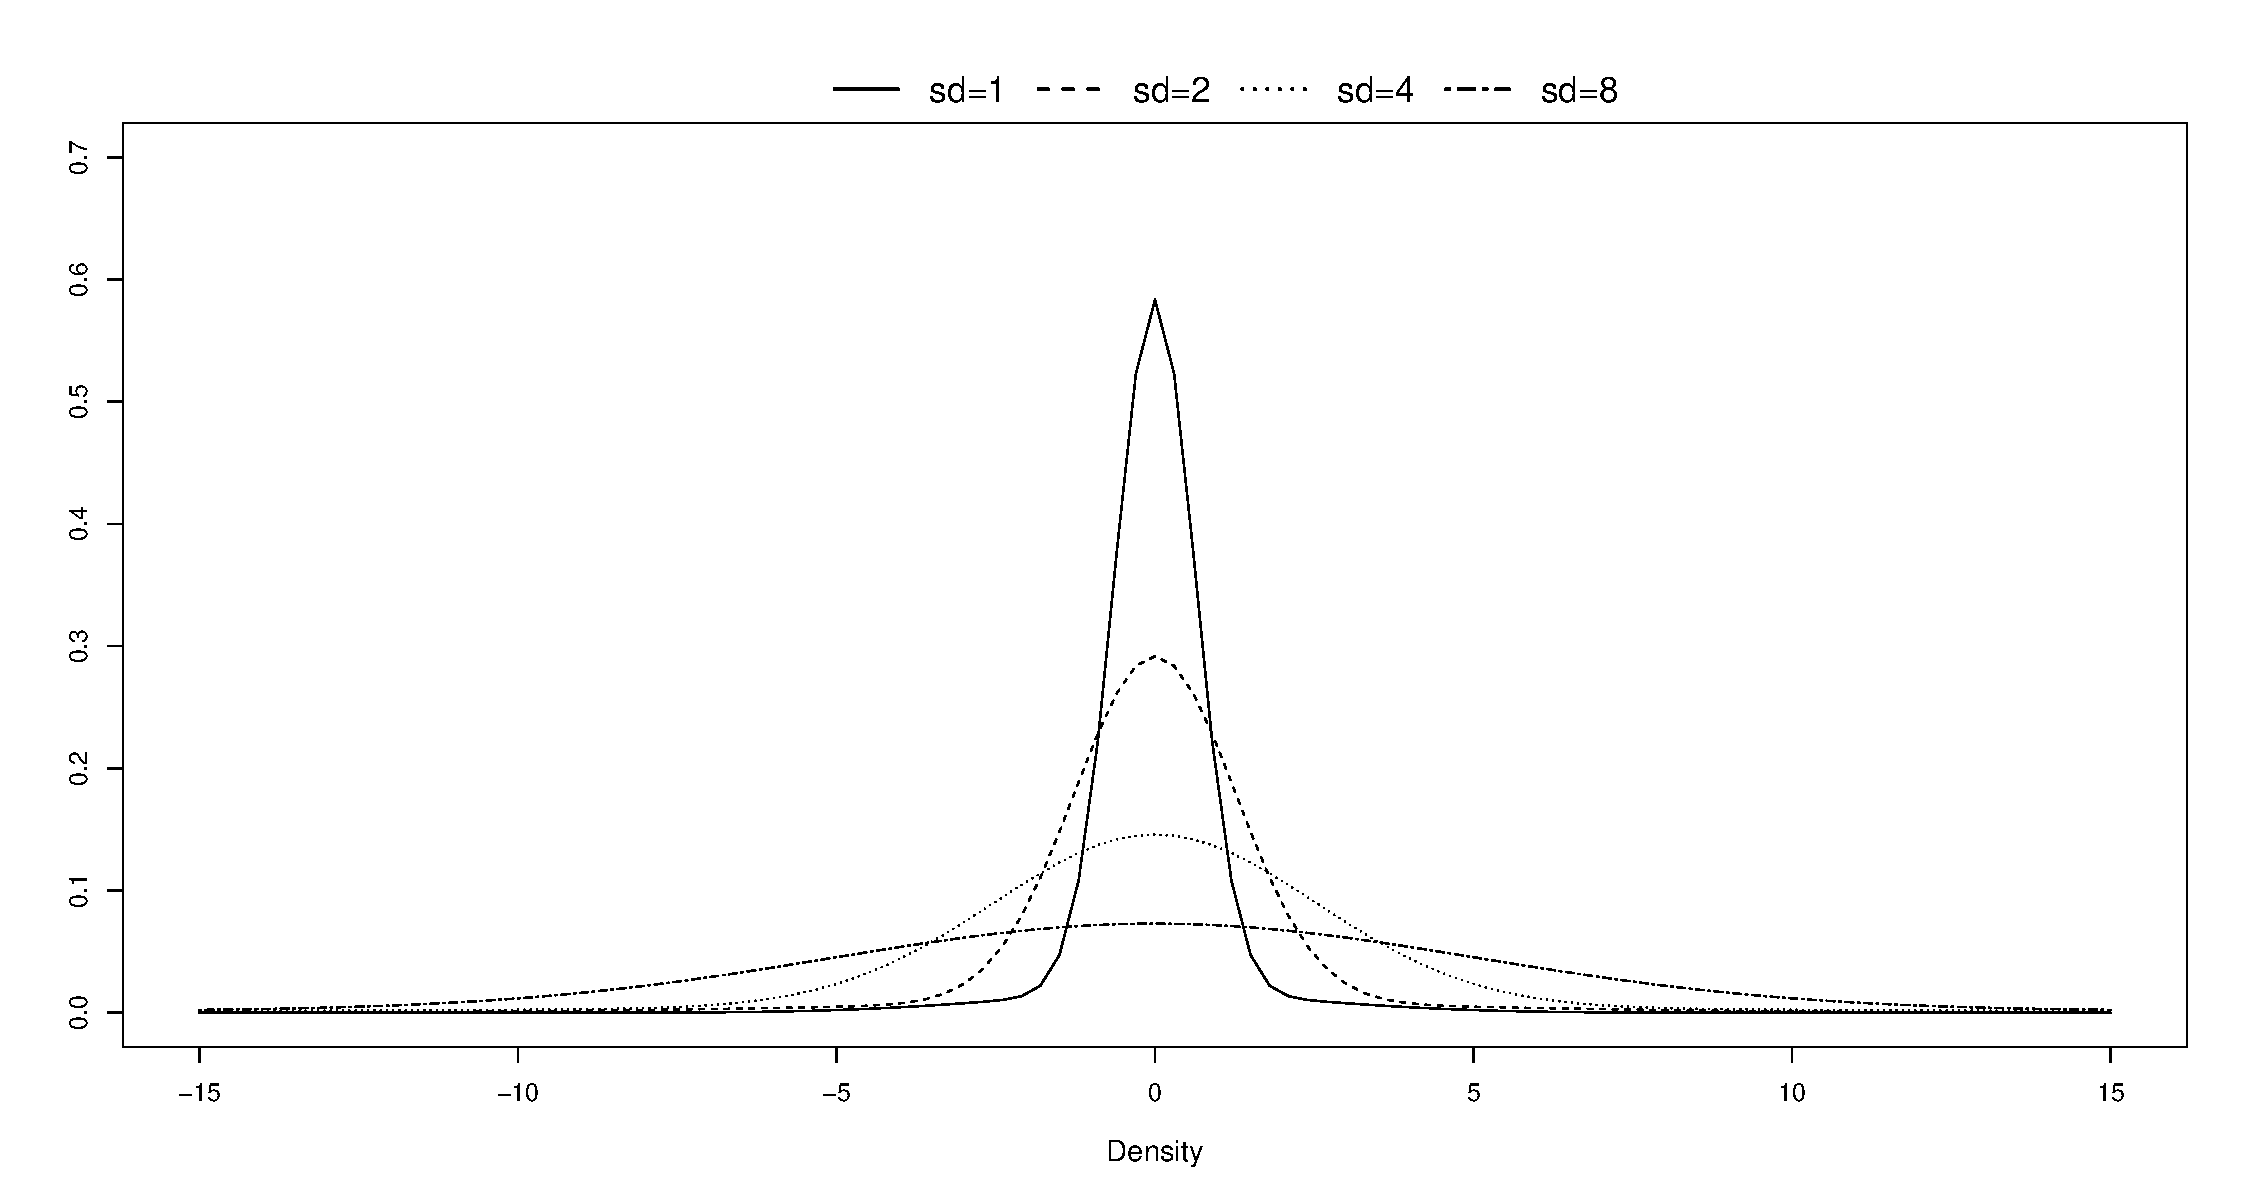
\includegraphics[width=400px]{W-test_files/figure-latex/unnamed-chunk-20-1} \caption{centered mixed normal probability density function, as a function of the population SD}\label{fig:unnamed-chunk-20}
\end{figure}

\begin{figure}
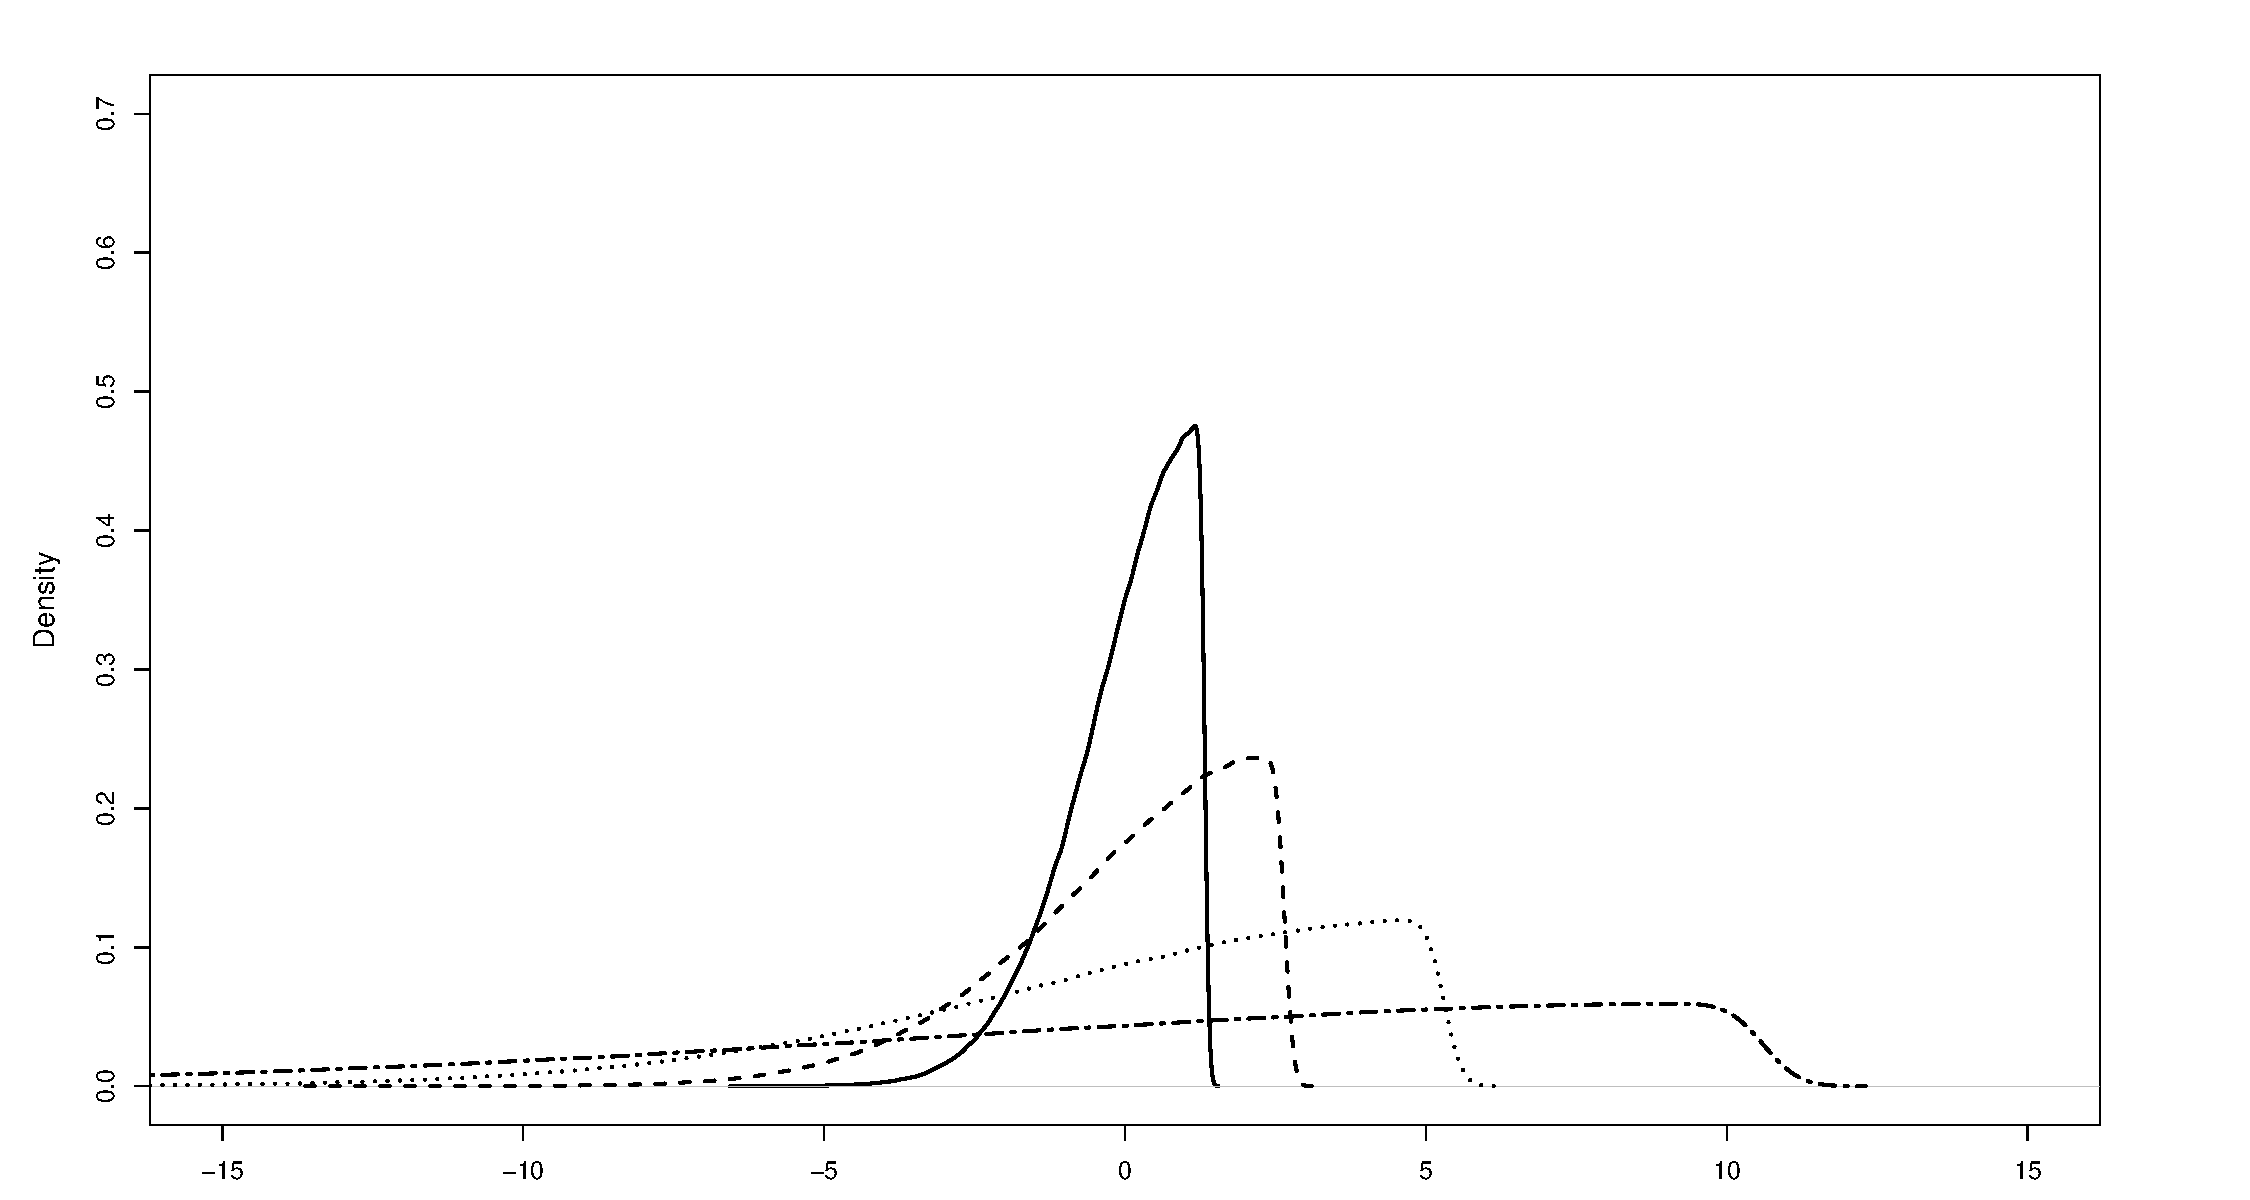
\includegraphics[width=400px]{W-test_files/figure-latex/unnamed-chunk-21-1} \caption{centered normal right skewed robability density function, as a function of the population SD}\label{fig:unnamed-chunk-21}
\end{figure}

\begin{figure}
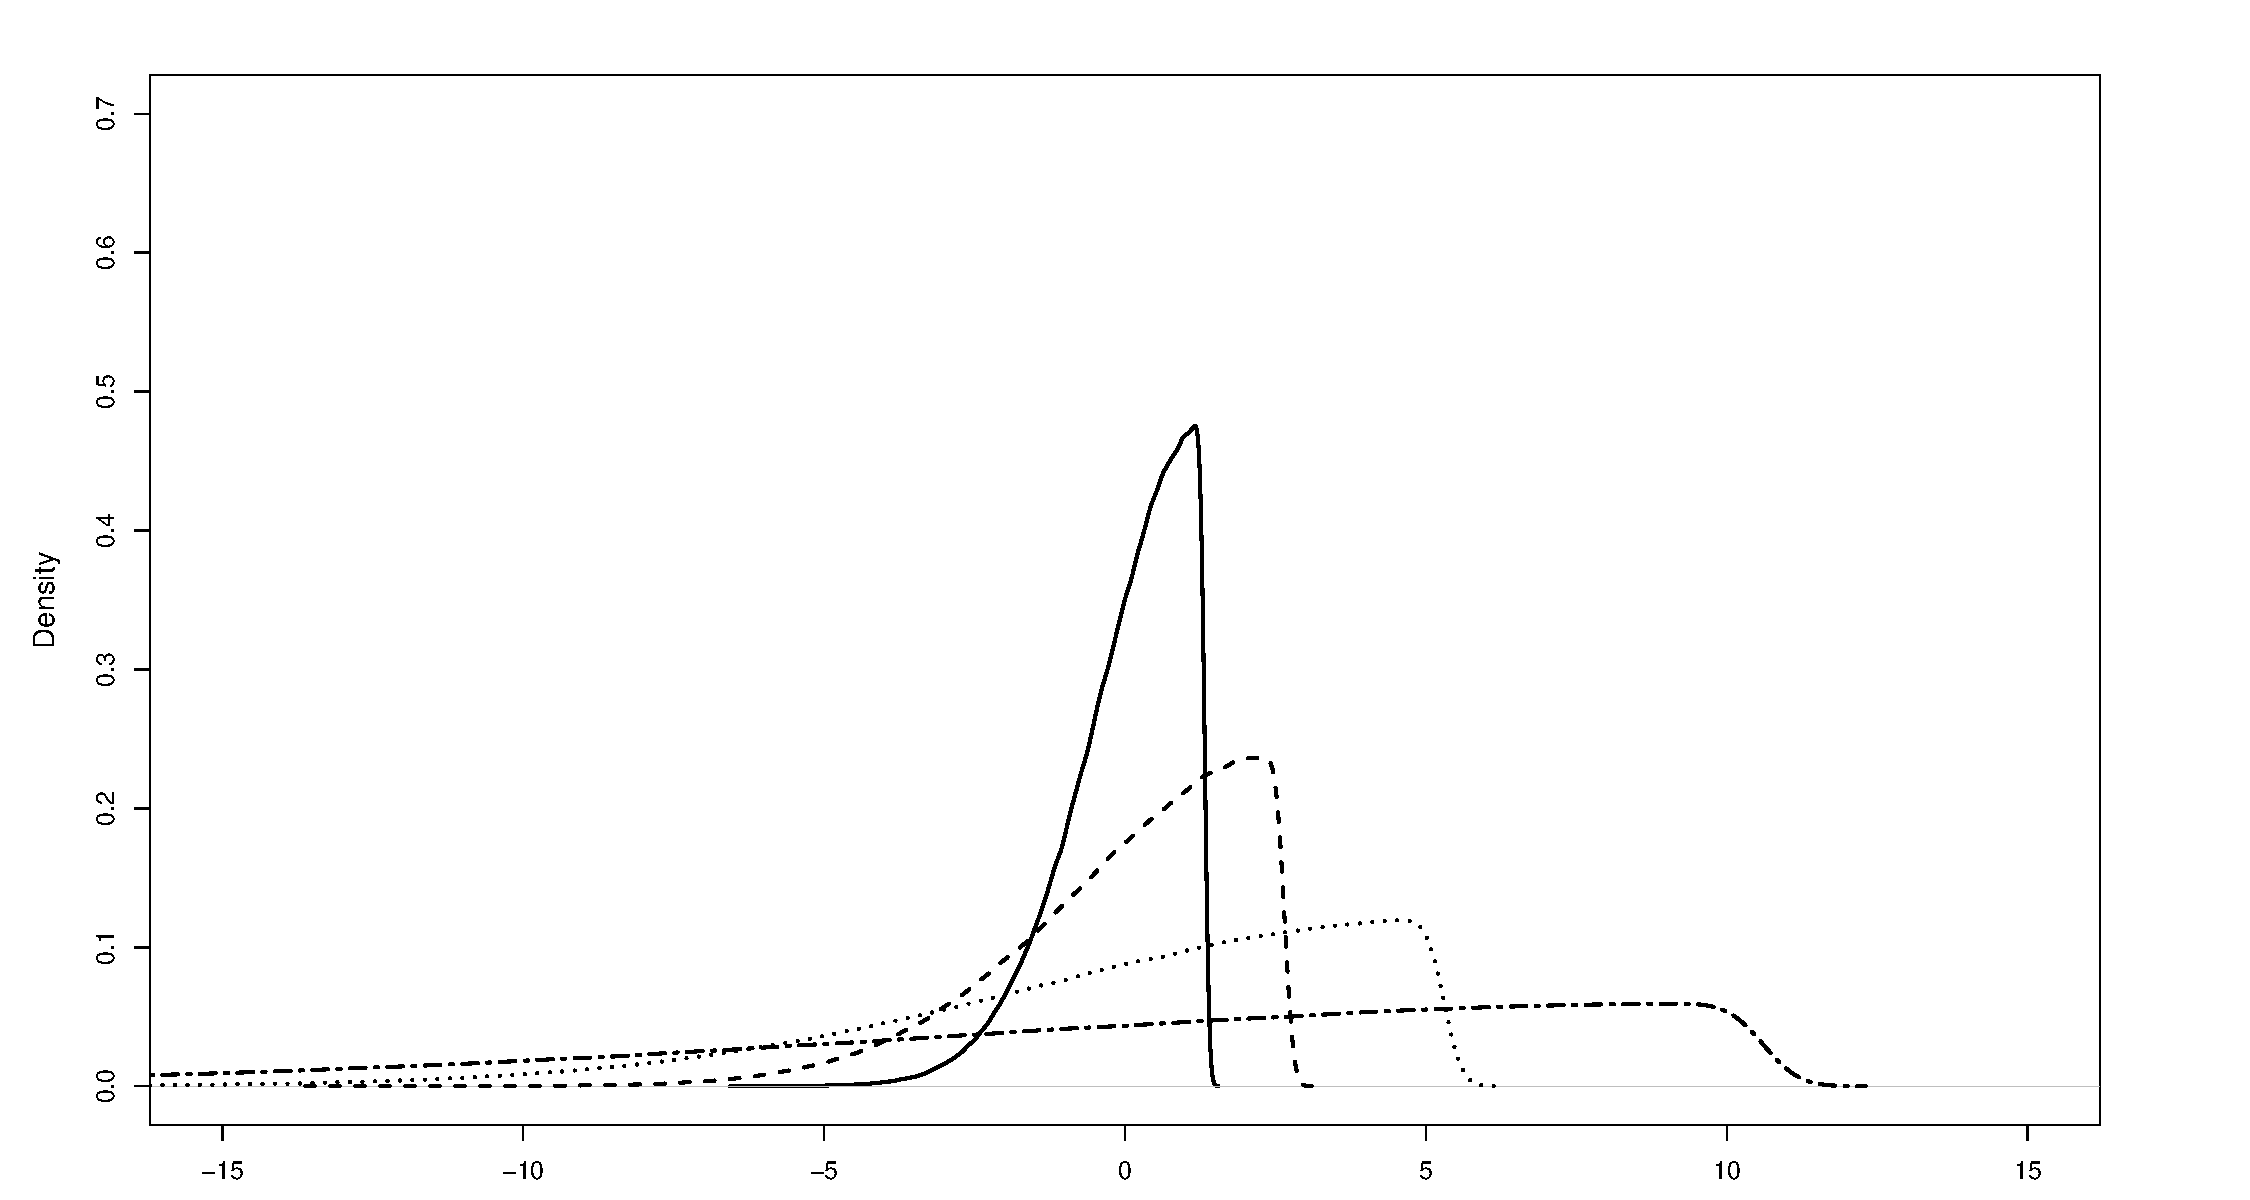
\includegraphics[width=400px]{W-test_files/figure-latex/unnamed-chunk-22-1} \caption{centered normal left skewed robability density function, as a function of the population SD}\label{fig:unnamed-chunk-22}
\end{figure}

\begin{figure}
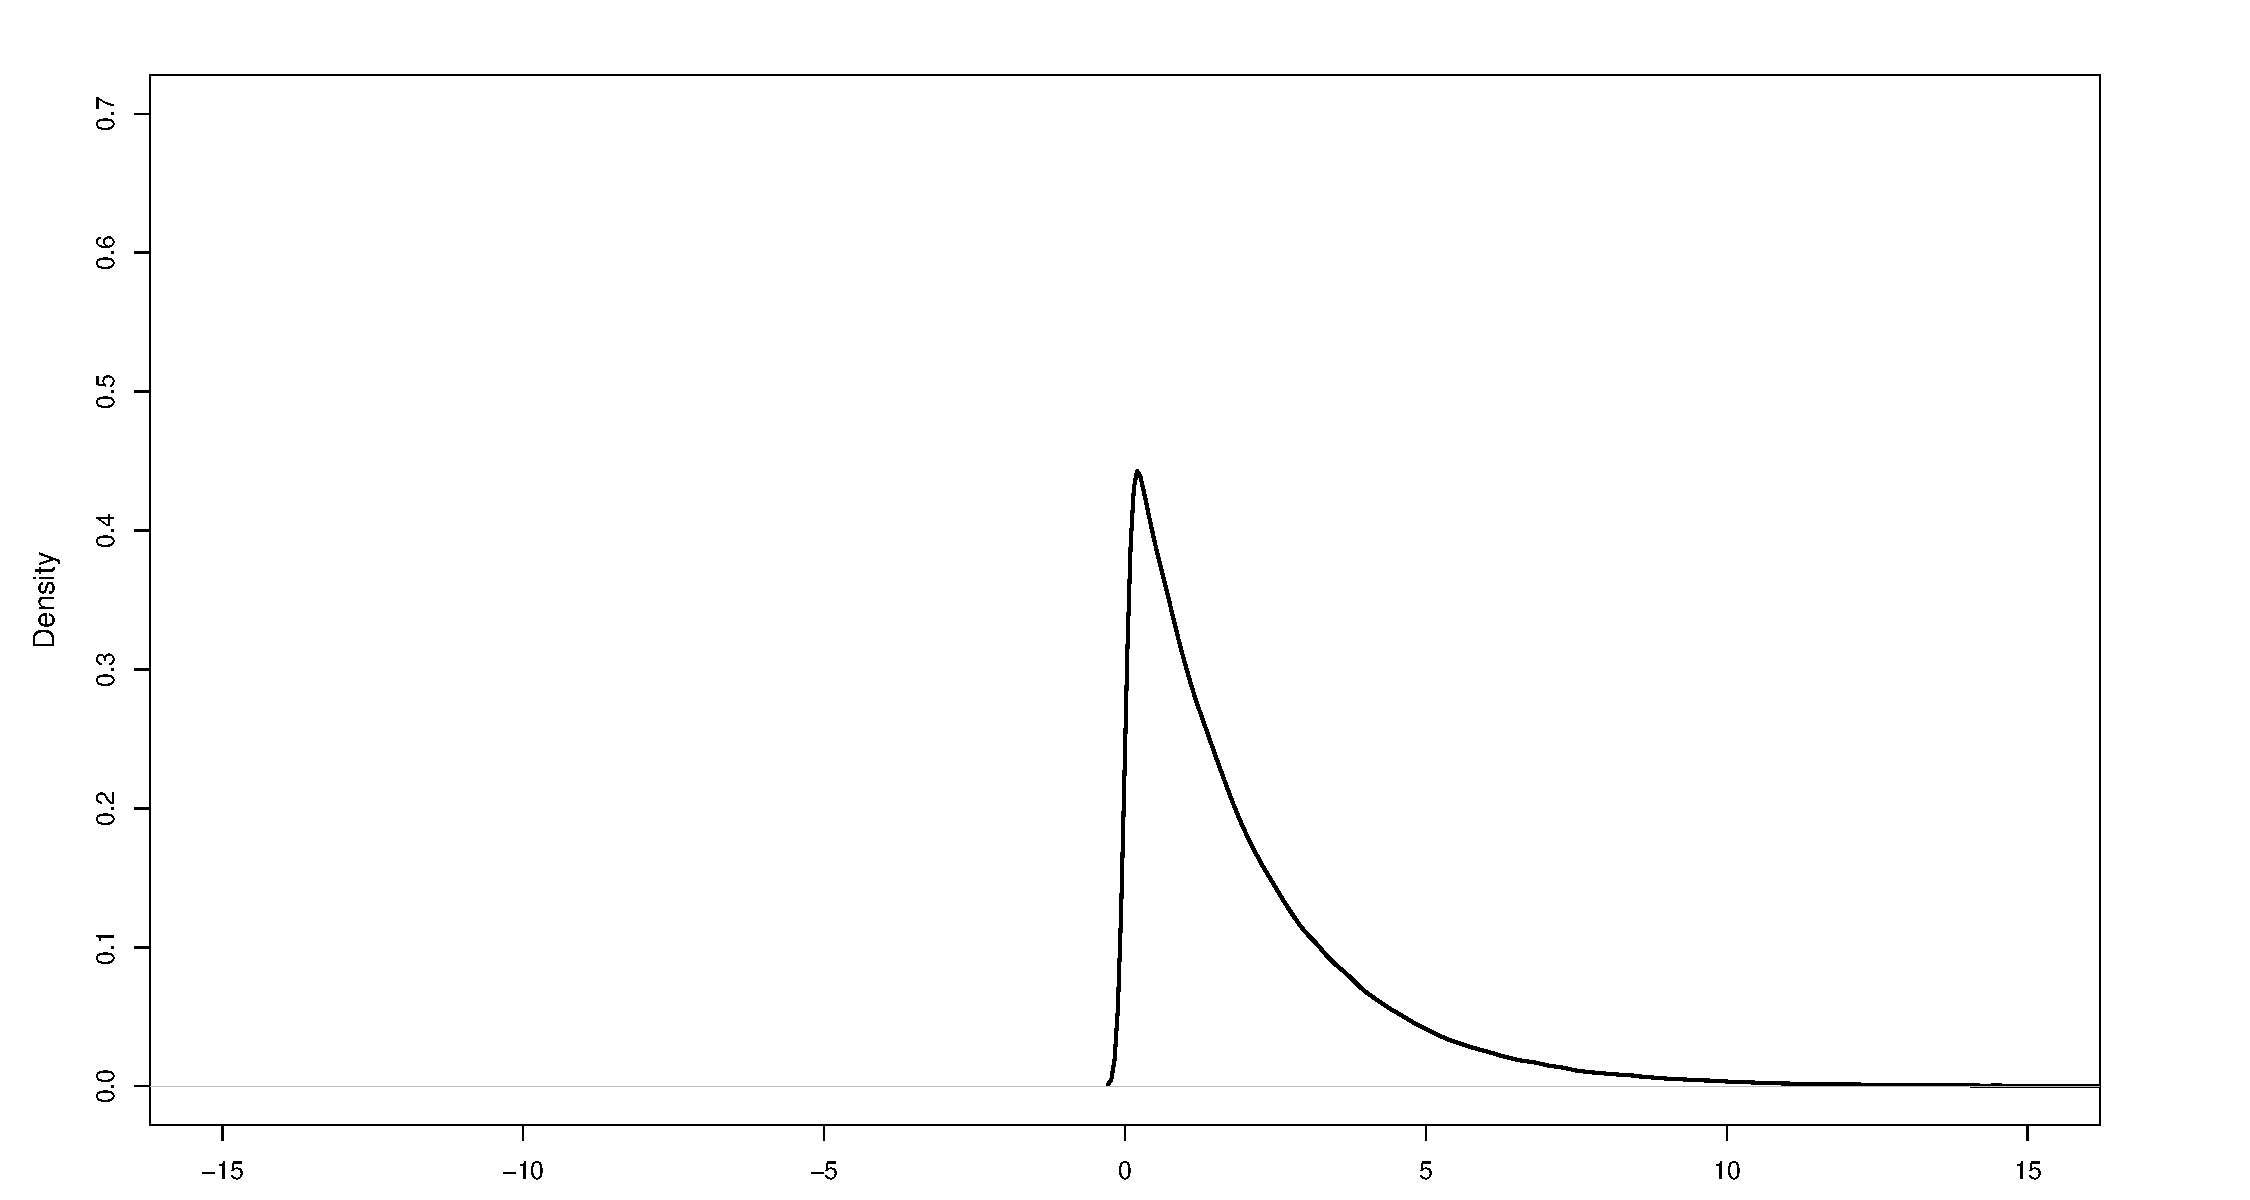
\includegraphics[width=400px]{W-test_files/figure-latex/unnamed-chunk-23-1} \caption{chi-squared with 2 degrees of freedom probability density function, as a function of the population SD}\label{fig:unnamed-chunk-23}
\end{figure}
\end{appendix}


\end{document}
